% ThinkAlgo — Counting and Probability — Grade 7
% Edition: teacher (with solutions), EN.  Generated by build_grade7.py — edit body/ and rebuild.
\documentclass[11pt]{article}
\newif\ifsol \soltrue
\usepackage{iftex}
\ifPDFTeX
  \usepackage[utf8]{inputenc}\usepackage[T5]{fontenc}
\else
  \usepackage{fontspec}
\fi
\usepackage[a4paper,top=2.95cm,headheight=1.5cm,headsep=0.45cm,bottom=3.1cm,left=1.9cm,right=1.9cm]{geometry}
\usepackage{amsmath,amssymb}
\usepackage{tikz}\usetikzlibrary{calc,shadows,shapes.geometric}
\usepackage[most]{tcolorbox}
\usepackage{enumitem}
\usepackage{array}
\usepackage{tabularx}
\usepackage{colortbl}
\usepackage{comment}
\usepackage{needspace}
\usepackage{fancyhdr}
\usepackage{fontawesome5}
\usepackage{graphicx}
\usepackage{microtype}
% PDF outline (bookmarks) so each chapter shows in the reader's outline — does not change the page layout
\usepackage[hidelinks,unicode,bookmarksnumbered=false,bookmarksopen=true,bookmarksopenlevel=0]{hyperref}
\usepackage{bookmark}
\usetikzlibrary{decorations.pathreplacing,arrows.meta,angles,quotes,patterns,positioning,through,intersections}

% ---------------- palette: navy family + subtle light tint; orange ONLY in the logo ----------------
% ----- EXACT palette from the user's original main (36).tex (vivid, not pale) -----
\definecolor{tmBlue}{RGB}{66,133,244}   % problem / header / section
\definecolor{tmGreen}{RGB}{52,168,83}   % solution
\definecolor{tmOrange}{RGB}{255,152,0}  % example
\colorlet{Navy}{tmBlue}                 % header rule / section heading / badge / divider
\definecolor{NavyD}{HTML}{222222}       % solution body text (dark, readable)
\colorlet{Gold}{Navy}
\colorlet{ProbBlue}{tmBlue}             % problem boxes
\colorlet{SolGreen}{tmGreen}            % solution boxes
\definecolor{AnsRed}{HTML}{E02424}      % vivid red for answers / totals
\definecolor{CardGreen}{HTML}{34A853}   % digit-card green
\definecolor{StarGold}{HTML}{F2B134}    % difficulty star (gold)
\definecolor{KidOrange}{HTML}{DE8A2C}   % logo accent only
\definecolor{Ink}{HTML}{1F2733}       % body text
\definecolor{Slate}{HTML}{5B6A82}     % muted labels
\definecolor{Line}{HTML}{C6D0DF}      % light hairlines / student boxes
\definecolor{Tint}{HTML}{EDF1F7}      % pale panel fill (worked solution / answer)
% aliases so older names keep working
\colorlet{TextDark}{Ink}\colorlet{TextGray}{Slate}\colorlet{Soft}{Slate}
\colorlet{CardLine}{Line}\colorlet{Teal}{Navy}\colorlet{ProbB}{Navy}\colorlet{SolG}{Navy}
% bright, kid-friendly colours for bar-model (sơ đồ đoạn thẳng) blocks
\definecolor{tmPurple}{RGB}{124,77,226}
\definecolor{tmTeal}{RGB}{0,150,136}
\definecolor{tmPink}{RGB}{233,30,99}
\AtBeginDocument{\color{Ink}}
\raggedbottom  % natural flow, even spacing (no stretched gaps)
\setlength{\parindent}{0pt}\setlength{\parskip}{0.18em}
\renewcommand{\arraystretch}{1.35}
\providecommand{\AnsWord}{Đáp số}

% ---------------- brand logo (original mark) ----------------
\newcommand{\logomark}[1]{\begin{tikzpicture}[baseline=-0.55ex,scale=#1]
  \draw[KidOrange,line width=1.5pt] (-0.27,0) .. controls (-0.27,0.23) and (0,0.23) .. (0,0)
        .. controls (0,-0.23) and (-0.27,-0.23) .. (-0.27,0);
  \draw[Navy,line width=1.5pt] (0.27,0) .. controls (0.27,0.23) and (0,0.23) .. (0,0)
        .. controls (0,-0.23) and (0.27,-0.23) .. (0.27,0);
\end{tikzpicture}}
% real brand logo image (gold infinity + "think algo" wordmark)
\newcommand{\logohead}{\IfFileExists{logo.png}{\includegraphics[height=1.35cm]{logo.png}}%
  {\raisebox{0.35cm}{\logomark{1.5}\hspace{0.5em}{\Large\bfseries\color{KidOrange}think\,\color{Navy}algo}}}}

% ---------------- running header (logo + Name/Date + topic) on EVERY page, single navy rule ----------------
\pagestyle{fancy}\fancyhf{}
\renewcommand{\headrulewidth}{1.4pt}\renewcommand{\footrulewidth}{0pt}
\renewcommand{\headrule}{{\color{Navy}\hrule height 1.3pt}}
\fancyhead[L]{\raisebox{-0.95cm}{\logohead}}
\fancyhead[R]{\setlength{\tabcolsep}{0pt}%
  \begin{tabular}{@{}r@{}}
    {\small\color{Ink}{\color{tmBlue}\faUserEdit}~\NameWord:~\rule{3.0cm}{0.5pt}\quad{\color{tmBlue}\faCalendarDay}~\DateWord:~\rule{1.9cm}{0.5pt}}\\[5pt]
    {\large\bfseries\color{Navy}\CurTopic}
  \end{tabular}}

% ---------------- footer (rounded page border + Topic/Grade + thinkalgo.com + page + tagline) ----------------
% NOTE: a remember-picture overlay must be placed DIRECTLY in \fancyfoot, NOT inside \def/\newcommand.
\fancyfoot[C]{\begin{tikzpicture}[remember picture, overlay]
  \draw[Navy!40, line width=1.4pt, rounded corners=12pt]
     ($(current page.north west)+(0.8cm,-0.8cm)$) rectangle ($(current page.south east)+(-0.8cm,0.45cm)$);
  \coordinate (FL) at ($(current page.south west)+(1.2cm, 2.18cm)$);
  \coordinate (FR) at ($(current page.south east)+(-1.2cm, 2.18cm)$);
  \draw[Navy!55, line width=1pt] (FL) -- (FR);
  \node[fill=white, draw=Navy, line width=1.2pt, rounded corners=8pt, font=\bfseries\small,
        text=Navy, inner xsep=11pt, inner ysep=4pt] at ($(current page.south)+(0,2.18cm)$) {{\color{tmBlue}\faGlobe}\ \ thinkalgo.com};
  \node[text=Slate, font=\footnotesize, anchor=north west, align=left, inner sep=0pt, text width=7.6cm]
        at ($(FL)+(0.1cm,-0.30cm)$) {{\color{tmBlue}\faTag}\ \TopicWord: \textbf{\color{Ink}\CurTopic}\\[1.5pt]{\color{tmBlue}\faGraduationCap}\ \DocGrade};
  \node[text=Slate, font=\footnotesize] at ($(current page.south)+(0,1.20cm)$) {\thepage};
  \node[text=Slate, font=\scriptsize, anchor=north east, align=right, inner sep=0pt, text width=7.4cm]
        at ($(FR)+(-0.1cm,-0.34cm)$) {{\normalsize\bfseries\color{Navy}ThinkAlgo}\ — From Math Thinking to Code};
\end{tikzpicture}}

% ---------------- page-1 lead-in (topic is already in the header; keep a slim spacer) ----------------
\newcommand{\titlehead}{\vspace*{-0.2cm}}
\providecommand{\CurTopic}{}

% chapter banner + sets the running-header topic. #1 = number, #2 = title
\newcommand{\chapterhead}[2]{\renewcommand{\CurTopic}{#2}%
  \setcounter{seccnt}{0}% each chapter is independent: section badges restart at 1
  \phantomsection\pdfbookmark[0]{#1. #2}{chap#1}\label{chap:#1}% add this chapter to the PDF outline + TOC ref
  \par\vspace{0.1cm}\noindent\begin{tikzpicture}[baseline=-0.5ex]
    \node[circle,fill=tmBlue,text=white,font=\Large\bfseries,minimum size=0.95cm,inner sep=0pt](cn){#1};
    \node[anchor=west,font=\LARGE\bfseries,text=tmBlue] at ([xshift=12pt]cn.east){#2};
  \end{tikzpicture}\par\vspace{4pt}\noindent\textcolor{tmBlue}{\rule{\linewidth}{2pt}}\par\vspace{0.5cm}}

% ---------------- section heading (outline navy number badge, no fill) ----------------
\newcounter{seccnt}
\newcommand{\shead}[1]{\par\vspace{0.7em}\refstepcounter{seccnt}%
  \noindent
\begin{tikzpicture}[baseline=-0.6ex]
    \node[circle,draw=Gold,line width=1.2pt,text=Gold,font=\bfseries,minimum size=1.05em,inner sep=1pt]{\theseccnt};
  \end{tikzpicture}\hspace{0.4em}{\large\bfseries\color{Navy} #1}\par\vspace{0.25em}}

% ============ boxes EXACTLY per the original main (36).tex: solid-blue PROBLEM, solid-orange EXAMPLE,
%              outline-green SOLUTION, all with drop shadow + rounded corners ============
% ---------------- knowledge box: white, tmBlue border + left accent + drop shadow ----------------
\newtcolorbox{knowbox}{enhanced,breakable,colback=white,colframe=tmBlue!70,boxrule=0.9pt,arc=5pt,
  left=12pt,right=11pt,top=6pt,bottom=6pt,drop shadow,
  borderline west={3.5pt}{0pt}{tmBlue}}

% ---------------- EXAMPLE (Ví dụ): SOLID ORANGE tab, white text ----------------
\newtcolorbox{exbox}[1]{enhanced,breakable,colback=white,colframe=tmOrange,boxrule=1pt,arc=5pt,
  left=12pt,right=11pt,top=14pt,bottom=7pt,drop shadow,
  attach boxed title to top left={xshift=10pt,yshift=-\tcboxedtitleheight/2},
  boxed title style={colback=tmOrange,colframe=tmOrange,arc=4pt,boxrule=0pt,drop shadow},
  title={#1},fonttitle=\bfseries\color{white}}
\newcommand{\guide}{\par\vspace{2pt}{\bfseries\color{tmBlue}\GuideWord}\par\nopagebreak}

% ---------------- PROBLEM (Bài): SOLID BLUE tab, white text ----------------
\newtcolorbox{probbox}[2]{enhanced,breakable,colback=white,colframe=tmBlue,boxrule=1pt,arc=5pt,
  left=12pt,right=10pt,top=14pt,bottom=7pt,drop shadow,
  attach boxed title to top left={xshift=10pt,yshift=-\tcboxedtitleheight/2},
  boxed title style={colback=tmBlue,colframe=tmBlue,arc=4pt,boxrule=0pt,drop shadow},
  fonttitle=\bfseries\color{white},title={\ProbWord\ #1\ifx\relax#2\relax\else#2\fi}}

% ---------------- SOLUTION (Lời giải): OUTLINE GREEN tab (white fill, green border + text) ----------------
% Teacher: a green tcolorbox. Student: the body is dropped entirely (comment pkg — robust with tables/\\).
\ifsol
  \newtcolorbox{solbox}{enhanced,breakable,colback=white,colframe=tmGreen,boxrule=1pt,arc=5pt,
    left=12pt,right=10pt,top=14pt,bottom=7pt,drop shadow,
    attach boxed title to top left={xshift=10pt,yshift=-\tcboxedtitleheight/2},
    boxed title style={colback=white,colframe=tmGreen,boxrule=1pt,arc=4pt,drop shadow},
    fonttitle=\bfseries\color{tmGreen!88!black},title={\SolTitle},before upper={\color{NavyD}}}
\else
  \excludecomment{solbox}
\fi

% ---------------- answer highlight: label green, value RED ----------------
\newcommand{\ans}[1]{\par\smallskip{\bfseries\color{tmGreen!88!black}\AnsWord:}\ {\bfseries\color{AnsRed}#1}\par}

% ---------------- digit cards (exact original style: fill=c!10, border=c!60!black, drop shadow) ----------------
% \digitcards{0/gray,1/cyan,2/green,3/cyan} : value/colour pairs
\newcommand{\digitcards}[1]{\begin{center}\begin{tikzpicture}[scale=0.7,transform shape,font=\sffamily]
  \def\dx{0}\foreach \v/\c in {#1}{
    \node[draw=\c!60!black,line width=1.5pt,fill=\c!10,rounded corners=4pt,
          minimum width=1cm,minimum height=1.4cm,drop shadow] at (\dx,0){\Huge\bfseries \v};
    \pgfmathsetmacro\dx{\dx+1.5}\xdef\dx{\dx}}
\end{tikzpicture}\end{center}}

% ---------------- student working space (white, light border) ----------------
\newcommand{\worksp}[1]{\ifsol\else\begin{tcolorbox}[colback=white,colframe=Line,boxrule=0.8pt,
  arc=5pt,height=\dimexpr#1+0.05cm\relax,left=8pt,right=8pt,top=4pt,bottom=4pt]{\footnotesize\color{Slate}\itshape\WorkWord}\end{tcolorbox}\fi}

% ---------------- \probsol{solution} : Teacher shows the green solution box; Student shows a BLANK
%   "Bài làm" box whose height matches that solution's height (writing room = work needed), so both
%   versions have identical per-problem height and paginate the same. ----------------
\newsavebox{\solmeasure}\newlength{\solht}
\newcommand{\probsol}[1]{%
  \begin{lrbox}{\solmeasure}\begin{minipage}{\dimexpr\linewidth-24pt\relax}#1\end{minipage}\end{lrbox}%
  \ifsol
    \begin{solbox}#1\end{solbox}%
  \else
    \setlength{\solht}{\dimexpr\ht\solmeasure+\dp\solmeasure+0.85cm\relax}%
    \ifdim\solht<1.35cm\setlength{\solht}{1.35cm}\fi
    \ifdim\solht>\StudentMaxWork\setlength{\solht}{\StudentMaxWork}\fi
    \begin{tcolorbox}[colback=white,colframe=Line,boxrule=0.8pt,arc=5pt,
      left=8pt,right=8pt,top=4pt,bottom=4pt,height=\solht]{\footnotesize\color{Slate}\itshape\WorkWord}\end{tcolorbox}%
  \fi}

% ---------------- practice divider: blue left accent bar, no fill ----------------
\newcommand{\dividerbar}[1]{\par\vspace{0.6em}\noindent
  \begin{tcolorbox}[enhanced,frame hidden,interior hidden,borderline west={5pt}{0pt}{ProbBlue},
    colback=white,left=12pt,right=12pt,top=5pt,bottom=5pt,arc=4pt]
  {\large\bfseries\color{ProbBlue} #1}\end{tcolorbox}\vspace{0.4em}}

% place-value choice-count diagram (Cambridge style): #1 = "label/count/note/color" list, #2 = result
% notes must NOT contain commas or slashes (they separate \foreach fields)
\newcommand{\countboxes}[2]{\begin{center}\begin{tikzpicture}[scale=0.62,transform shape,font=\sffamily]
  \def\xx{0}%
  \foreach \lab/\cnt/\note/\col [count=\i] in {#1}{%
    \ifnum\i>1\relax \node[text=gray,font=\Huge] at (\xx-1.8,0){$\times$};\fi
    \node[draw=\col!65,fill=\col!8,rounded corners=3pt,line width=1pt,minimum width=2.7cm,minimum height=1.7cm] at (\xx,0){};
    \node[text=\col!85,font=\bfseries] at (\xx,0.58){\lab};
    \node[text=\col!88,font=\Huge\bfseries] at (\xx,-0.1){\cnt};
    \node[text=gray,font=\scriptsize] at (\xx,-1.05){\note};
    \pgfmathsetmacro\xx{\xx+3.6}\xdef\xx{\xx}}%
  \node[text=gray,font=\Huge] at (\xx-1.8,0){$=$};
  \node[text=red,font=\Huge\bfseries] at (\xx,0){#2};
\end{tikzpicture}\end{center}}

% ======== bar model (sơ đồ đoạn thẳng): lightly-rounded blocks, darker border, tiny gaps, bright colours ========
% one block: \blk{x1}{x2}{yc}{height}{colour}{label}  (a small gap is left on each side)
\newcommand{\blk}[6]{%
  \draw[rounded corners=1.3pt,fill=#5!16,draw=#5!80!black,line width=1pt]
    (#1+0.045,#3-#4/2) rectangle (#2-0.045,#3+#4/2);
  \node[font=\small\bfseries,text=#5!52!black] at ({(#1+#2)/2},#3){#6};}
% measurement with a double-headed ARROW (not a brace) + label above the span: \brcup{x1}{x2}{y}{label}
\newcommand{\brcup}[4]{%
  \draw[<->,>=stealth,tmBlue!72!black,line width=0.7pt] (#1+0.05,#3)--(#2-0.05,#3);
  \node[above=-1.5pt,font=\footnotesize,text=tmBlue!58!black] at ({(#1+#2)/2},#3){#4};}
% measurement with a double-headed ARROW + label below the span: \brcdn{x1}{x2}{y}{label}
\newcommand{\brcdn}[4]{%
  \draw[<->,>=stealth,tmBlue!72!black,line width=0.7pt] (#1+0.05,#3)--(#2-0.05,#3);
  \node[below=-1.5pt,font=\footnotesize,text=tmBlue!58!black] at ({(#1+#2)/2},#3){#4};}
% row label at the left of a bar: \rowlab{x}{y}{text}
\newcommand{\rowlab}[3]{\node[anchor=east,font=\small\bfseries,text=Ink] at (#1,#2){#3};}
% vertical right-pointing CURLY BRACE spanning two stacked bars: \vbrace{x}{ytop}{ybot}{label}
\newcommand{\vbrace}[4]{%
  \pgfmathsetmacro\ym{(#2+#3)/2}%
  \draw[tmBlue!72!black,line width=0.9pt,line cap=round]
    (#1,#2) .. controls (#1+0.18,#2) and (#1+0.18,#2-0.18) .. (#1+0.18,#2-0.22)
    -- (#1+0.18,{\ym+0.22})
    .. controls (#1+0.18,\ym) and (#1+0.30,{\ym+0.08}) .. (#1+0.42,\ym)
    .. controls (#1+0.30,{\ym-0.08}) and (#1+0.18,\ym) .. (#1+0.18,{\ym-0.22})
    -- (#1+0.18,#3+0.22)
    .. controls (#1+0.18,#3+0.18) and (#1+0.18,#3) .. (#1,#3);
  \node[right=4pt,font=\footnotesize,text=tmBlue!58!black] at (#1+0.42,\ym){#4};}
% blank 3x3 grid for a problem statement (student fills it in)
\newcommand{\blankgrid}{
\begin{tikzpicture}[font=\sffamily]
  \foreach \r in {0,1,2}{\foreach \c in {0,1,2}{
    \draw[rounded corners=1.3pt,fill=Tint,draw=Slate!55,line width=0.9pt]
      (\c+0.05,\r+0.05) rectangle (\c+0.95,\r+0.95);}}
\end{tikzpicture}}
% wrapper: LEFT-aligned (not centred), a little air above/below
\newenvironment{barfig}{\par\vspace{3pt}\noindent\kern0.35cm\begin{tikzpicture}[font=\sffamily,>=stealth]}%
  {\end{tikzpicture}\par\vspace{3pt}}
% wrapper: CENTRED (for illustrative diagrams in theory / examples)
\newenvironment{barfigC}{\par\vspace{3pt}\begin{center}\begin{tikzpicture}[font=\sffamily,>=stealth]}%
  {\end{tikzpicture}\end{center}\vspace{2pt}}

% ---------------- difficulty stars (nicely drawn) : \stars{1}=hard, \stars{2}=very hard ----------------
\newcommand{\diffstar}{\tikz[baseline=-0.55ex]{\node[star,star points=5,star point ratio=0.46,
  draw=StarGold!72!black,fill=StarGold,line width=0.3pt,inner sep=1.75pt]{};}}
\newcommand{\stars}[1]{\ifcase#1\or\kern2pt\diffstar\or\kern2pt\diffstar\kern1.5pt\diffstar\fi}

\newcommand{\nd}[1]{\overline{#1}}

% number line: #1 last index, #2 ticks "i/label", #3 open (excluded) indices, #4 filled (solution) indices
\newcommand{\numlinex}[4]{\begin{center}\begin{tikzpicture}[x=1.55cm,>=stealth]
  \draw[->,thick,Navy](-0.45,0)--(#1+0.45,0);
  \foreach \i/\lab in {#2}{\draw[Navy,line width=0.8pt](\i,0.08)--(\i,-0.08);
     \node[below,font=\small,text=Ink]at(\i,-0.1){\lab};}
  \foreach \i in {#3}{\draw[Navy,fill=white,line width=1pt](\i,0)circle(2.3pt);}
  \foreach \i in {#4}{\fill[KidOrange](\i,0)circle(2.7pt);}
\end{tikzpicture}\end{center}}


% ======================================================================
% Grade 7 additions (shared by all four editions)
% ======================================================================
% student edition: blank "work" box height = min(solution height, this cap)
\newlength{\StudentMaxWork}\setlength{\StudentMaxWork}{7.5cm}

% ThinkAlgo tip box (label set per language by \TipWord)
\newtcolorbox{tipbox}{enhanced,breakable,colback=StarGold!8,colframe=StarGold!75!black,boxrule=1pt,arc=4pt,
  left=11pt,right=10pt,top=6pt,bottom=6pt,
  before upper={\textbf{\color{StarGold!65!black}\faLightbulb\ \TipWord}\ }}

% "Recall" box: re-states a piece of theory inside a solution / example
\newtcolorbox{recallbox}{enhanced,breakable,colback=tmBlue!5,colframe=tmBlue!45,boxrule=0.6pt,arc=3pt,
  left=8pt,right=8pt,top=4pt,bottom=4pt,
  before upper={\textbf{\color{tmBlue!80!black}\faBookOpen\ \RecallWord}\ }}

% "Why is it true? / Proof" box
\newtcolorbox{proofbox}{enhanced,breakable,colback=tmPurple!4,colframe=tmPurple!45,boxrule=0.6pt,arc=3pt,
  left=8pt,right=8pt,top=4pt,bottom=4pt,
  before upper={\textbf{\color{tmPurple!85!black}\faSearch\ \ProofWord}\ },
  after upper={\hfill$\square$}}

% "Common mistake" box
\newtcolorbox{warnbox}{enhanced,breakable,colback=AnsRed!4,colframe=AnsRed!45,boxrule=0.6pt,arc=3pt,
  left=8pt,right=8pt,top=4pt,bottom=4pt,
  before upper={\textbf{\color{AnsRed!85!black}\faExclamationTriangle\ \WarnWord}\ }}

% "Note for parents" box (short hint on how to explain the idea at home)
\newtcolorbox{parentbox}{enhanced,breakable,colback=tmTeal!5,colframe=tmTeal!50,boxrule=0.6pt,arc=3pt,
  left=8pt,right=8pt,top=4pt,bottom=4pt,
  before upper={\textbf{\color{tmTeal!80!black}\faUsers\ \ParentWord}\ }}

% numbered step inside a solution:  \step{1}{Short title}  -> "Bước 1. Short title"
\newcommand{\step}[2]{\par\smallskip\noindent{\bfseries\color{tmBlue!85!black}\StepWord~#1.}\ {\bfseries #2}\par\nopagebreak}
% verification line:  \verify{...}
\newcommand{\verify}[1]{\par\smallskip\noindent{\bfseries\color{tmGreen!80!black}\faCheckCircle\ \CheckWord}\ #1\par}

% multiple-choice options
% \choices{..}{..}{..}{..}{..}      : five short options on one line
% \choicesII{..}{..}{..}{..}{..}    : two/three per line (medium length)
% \choicesL{..}{..}{..}{..}{..}     : one option per line (long text)
\newcommand{\choices}[5]{\par\smallskip\noindent
  \begin{tabularx}{\linewidth}{@{}XXXXX@{}}(A)\ #1&(B)\ #2&(C)\ #3&(D)\ #4&(E)\ #5\end{tabularx}\par}
\newcommand{\choicesII}[5]{\par\smallskip\noindent
  \begin{tabularx}{\linewidth}{@{}XXX@{}}(A)\ #1&(B)\ #2&(C)\ #3\\(D)\ #4&(E)\ #5&\end{tabularx}\par}
\newcommand{\choicesL}[5]{\par\smallskip\noindent
  \begin{tabular}{@{}l@{}}(A)\ #1\\(B)\ #2\\(C)\ #3\\(D)\ #4\\(E)\ #5\end{tabular}\par}

% centred figure inside a problem / solution
\newenvironment{figC}{\par\vspace{2pt}\begin{center}\begin{tikzpicture}[font=\sffamily\small,>=stealth,line join=round]}%
  {\end{tikzpicture}\end{center}\vspace{1pt}}

\def\DocGrade{Grade 7}
\def\ProbWord{Problem}
\def\SolWord{Solution.}
\def\GuideWord{Guided solution.}
\def\PageWord{Page}
\def\NameWord{Name}
\def\DateWord{Date}
\def\SolTitle{Detailed solution}
\def\WorkWord{Your work:}
\def\TopicWord{Topic}
\def\AnsWord{Answer}
\def\TipWord{ThinkAlgo Tip.}
\def\RecallWord{Recall.}
\def\ProofWord{Why is it true?}
\def\WarnWord{Common mistake.}
\def\ParentWord{Note for parents.}
\def\StepWord{Step}
\def\CheckWord{Check:}

\def\DocTopic{Counting and Probability}
\begin{document}
\titlehead
\chapterhead{3}{Counting and Probability}

% ---------------- part a ----------------
% ======================================================================
% Topic 3 -- Counting and Probability -- part a (theory, examples, problems 1--15)
% ======================================================================
% helper: spinner with 6 equal sectors, labels clockwise starting from the top-left sector
\providecommand{\cpSpinSix}[6]{%
  \foreach \a in {90,150,210,270,330,30}{\draw[Ink,line width=0.8pt] (0,0)--(\a:1.1);}
  \draw[Ink,line width=1pt] (0,0) circle (1.1);
  \node[font=\itshape\large] at (120:0.72){#1};
  \node[font=\itshape\large] at (60:0.72){#2};
  \node[font=\itshape\large] at (0:0.72){#3};
  \node[font=\itshape\large] at (-60:0.72){#4};
  \node[font=\itshape\large] at (-120:0.72){#5};
  \node[font=\itshape\large] at (180:0.72){#6};
  \draw[-{Stealth[length=7pt]},line width=1.6pt,Ink] (0,0)--(266:0.98);
  \fill[Ink] (0,0) circle (1.6pt);}
% helper: a regular octagon centred at (#1,#2), width 1
\providecommand{\cpOct}[2]{%
  \draw[Ink,line width=0.8pt,fill=tmBlue!8] (#1-0.2071,#2+0.5)--(#1+0.2071,#2+0.5)--(#1+0.5,#2+0.2071)--(#1+0.5,#2-0.2071)
     --(#1+0.2071,#2-0.5)--(#1-0.2071,#2-0.5)--(#1-0.5,#2-0.2071)--(#1-0.5,#2+0.2071)--cycle;}
% helper: small square (diamond) between four octagons, centre (#1,#2)
\providecommand{\cpDia}[2]{%
  \draw[Ink,line width=0.8pt,fill=tmOrange!35] (#1,#2+0.2929)--(#1+0.2929,#2)--(#1,#2-0.2929)--(#1-0.2929,#2)--cycle;}


\begin{knowbox}
\textbf{The big idea.} In this topic every problem comes back to \emph{one core skill}: \textbf{counting correctly} -- missing nothing and counting nothing twice.
\begin{itemize}[leftmargin=1.2em,itemsep=1pt,topsep=2pt]
\item \textbf{Counting} answers the question ``\emph{how many?}'': how many numbers, how many seating arrangements, how many rectangles in a figure, how many toothpicks\ldots
\item \textbf{Probability} answers the question ``\emph{how likely is it?}''. When all outcomes are equally likely, we only need to \emph{count twice}:
\[
\text{Probability}=\frac{\text{number of favourable outcomes}}{\text{number of all possible outcomes}} .
\]
\item Our counting tools: \textbf{systematic listing}, \textbf{tables}, \textbf{tree diagrams}, the \textbf{multiplication rule}, \textbf{splitting into cases} (the addition rule), \textbf{finding a pattern} and \textbf{reasoning by elimination}.
\end{itemize}
Always ask yourself three questions before starting: \emph{(1) How many possible outcomes are there altogether? (2) Are these outcomes ``fair'' (equally likely)? (3) How many of them satisfy the requirement?}
\end{knowbox}

\begin{figC}
\node[draw=tmBlue,fill=tmBlue!10,rounded corners=4pt,line width=1pt,minimum width=3.2cm,minimum height=0.9cm,font=\sffamily\bfseries] (D) at (0,0) {COUNT CORRECTLY};
\node[draw=tmGreen,fill=tmGreen!10,rounded corners=4pt,line width=1pt,minimum width=3.2cm,minimum height=0.9cm,font=\sffamily\bfseries] (X) at (6,0) {PROBABILITY};
\draw[->,line width=1.2pt,Ink] (D)--node[above,font=\footnotesize]{favourable / all}(X);
\foreach \t/\y in {Listing -- tables/1.9,Tree diagrams/1.2,Multiplication rule/0.5,Splitting into cases/-0.2,Finding a pattern/-0.9,Elimination/-1.6}{
  \node[draw=tmOrange,fill=tmOrange!10,rounded corners=3pt,font=\footnotesize,minimum width=2.9cm] at (-4.3,\y-0.15) (n) {\t};
  \draw[->,tmOrange!80!black] (n.east)--(D.west);}
\end{figC}
\vspace{0.3cm}

% ----------------------------------------------------------------------
\shead{Experiments, outcomes, events and probability}
\begin{knowbox}
\textbf{Key words.}
\begin{itemize}[leftmargin=1.2em,itemsep=1pt,topsep=2pt]
\item A \textbf{random experiment} is an action for which we know in advance \emph{all the possible outcomes}, but not \emph{which outcome will happen}. Examples: rolling a die, tossing a coin, spinning a spinner, drawing a marble from a bag without looking.
\item The \textbf{set of possible outcomes} is the list of \emph{all} outcomes. Rolling a die: $\{1,2,3,4,5,6\}$ -- $6$ outcomes. Tossing a coin: $\{\text{heads},\ \text{tails}\}$ -- $2$ outcomes.
\item An \textbf{event} is something we are interested in, for example ``rolling an even number''. The outcomes that make the event happen are called \textbf{favourable outcomes} for the event. The event ``rolling an even number'' has $3$ favourable outcomes: $2,4,6$.
\item Outcomes are \textbf{equally likely} if none of them is ``easier to get'' than another (a fair die, a fair coin, equal sectors on a spinner, marbles of identical shape and size).
\end{itemize}
\textbf{Probability formula} (when the outcomes are equally likely):
\[
P(\text{event})=\frac{\text{number of outcomes favourable to the event}}{\text{number of all possible outcomes}} .
\]
\textbf{Properties.} The number of favourable outcomes is between $0$ and the total number of outcomes, so always $0\le P\le 1$.
\begin{itemize}[leftmargin=1.2em,itemsep=1pt,topsep=2pt]
\item $P=0$: an \emph{impossible} event (for example rolling a $7$ on a die).
\item $P=1$: a \emph{certain} event (for example rolling a number less than $7$).
\end{itemize}
\end{knowbox}

\begin{proofbox}
Why a division? Suppose there are $n$ equally likely outcomes. The total ``chance'' $1$ (one of the outcomes is sure to happen) is shared \emph{equally} among $n$ outcomes, so each outcome has probability $\dfrac{1}{n}$. If the event has $k$ favourable outcomes, we add $k$ equal parts: $\dfrac1n+\dfrac1n+\dots+\dfrac1n=\dfrac{k}{n}$.
\end{proofbox}

\begin{figC}
\begin{scope}
\cpSpinSix{1}{2}{3}{4}{5}{6}
\node[font=\footnotesize,align=center] at (0,-1.55){Spinner with $6$ equal sectors:\\ each sector has probability $\frac16$};
\end{scope}
\begin{scope}[xshift=5cm]
\draw[Ink,line width=1pt,rounded corners=6pt] (-1.3,1)--(-1.2,-1)--(1.2,-1)--(1.3,1);
\foreach \x/\y/\c in {-0.8/-0.7/AnsRed,-0.3/-0.7/AnsRed,0.2/-0.7/tmOrange,0.7/-0.7/tmOrange,-0.55/-0.25/tmOrange,
   -0.05/-0.25/tmOrange,0.45/-0.25/tmOrange,-0.3/0.2/tmBlue,0.2/0.2/tmBlue,0.7/0.2/tmBlue,-0.8/0.2/tmBlue}{
  \shade[ball color=\c] (\x,\y) circle (0.22);}
\node[font=\footnotesize,align=center] at (0,-1.55){Bag with $2$ red, $5$ yellow, $4$ blue:\\ $P(\text{red})=\frac{2}{11}$};
\end{scope}
\end{figC}

\begin{warnbox}
\textbf{Count \emph{objects}, not \emph{kinds}.} The bag above has $3$ \emph{colours} but $11$ \emph{marbles}. The probability of drawing a red marble is $\dfrac{2}{11}$, \textbf{not} $\dfrac13$. Each marble is one equally likely outcome; the three colours are not equally likely (yellow has more marbles, so it is easier to draw).
\end{warnbox}

\begin{warnbox}
\textbf{Use the formula only when the outcomes are equally likely.} On a spinner with big and small sectors, the sectors are \emph{not} equally likely. Then the probability of landing in a sector equals \emph{the fraction of the whole circle} that the sector takes up, that is $\dfrac{\text{central angle of the sector}}{360^\circ}$. For example a sector with angle $90^\circ$ has probability $\dfrac{90}{360}=\dfrac14$.
\end{warnbox}

\begin{tipbox}
In multiple-choice questions the answer may be written in \emph{unsimplified} form, such as $\dfrac{2}{6}$ instead of $\dfrac13$. Compare the values of the fractions, not just how they look. On the other hand, when you write your own solution, simplify your final answer.
\end{tipbox}

% ----------------------------------------------------------------------
\shead{Complementary events. Finding a quantity from a probability}
\begin{knowbox}
\textbf{Complementary event.} The event ``$A$ does \emph{not} happen'' is called the complement of $A$. We have
\[
P(\text{not } A)=1-P(A).
\]
Example: rolling a die, $P(\text{a }6)=\dfrac16$, so $P(\text{not a }6)=1-\dfrac16=\dfrac56$.

\medskip
\textbf{Finding a quantity from a probability.} From the probability formula we get
\[
\text{number of favourable outcomes}=P\times\text{number of all outcomes}.
\]
Example: a bag has $20$ sweets and the probability of drawing a lemon sweet is $\dfrac{3}{4}$; then there are $20\times\dfrac34=15$ lemon sweets.

\medskip
\textbf{When the quantities change} (drawn and \emph{not replaced}, eaten, added\ldots): \textbf{recount both the numerator and the denominator} before computing the probability for the next draw.
\end{knowbox}

\begin{proofbox}
Suppose there are $n$ outcomes, of which $k$ are favourable to $A$. Each of the remaining $n-k$ outcomes makes $A$ \emph{not} happen. So
$P(\text{not }A)=\dfrac{n-k}{n}=\dfrac{n}{n}-\dfrac{k}{n}=1-P(A)$.
\end{proofbox}

\begin{warnbox}
A box has $10$ red and $10$ blue marbles. A student takes out $1$ blue marble and does \emph{not put it back}. What is the probability that the next marble is red?
\begin{itemize}[leftmargin=1.2em,itemsep=1pt,topsep=2pt]
\item \textbf{Wrong:} ``still $\dfrac{10}{20}$'' (forgetting that the box now has one marble fewer).
\item \textbf{Right:} $19$ marbles are left, and all $10$ red ones are still there, so the probability is $\dfrac{10}{19}$.
\end{itemize}
\end{warnbox}

\begin{parentbox}
Do a real experiment with sweets or bottle caps of different colours: put them in a cloth bag, count together ``how many are there altogether, how many are red'', then take one out and ask the same two questions again. Your child will see for themselves that both the numerator and the denominator change.
\end{parentbox}

% ----------------------------------------------------------------------
\shead{Systematic listing: lists, tables and tree diagrams}
\begin{knowbox}
When the number of possibilities is not too large, the safest method is to \textbf{list them all}. To list without missing or repeating anything, we need \textbf{an order}:
\begin{itemize}[leftmargin=1.2em,itemsep=1pt,topsep=2pt]
\item An \textbf{ordered list} (from smallest to largest, alphabetically\ldots). Example: the two-digit numbers with different digits made from $1,2,3$: $12,13,21,23,31,32$ -- ordered by the tens digit.
\item A \textbf{two-way table} when the experiment has \emph{two stages} (rolling two dice, choosing a main dish and a dessert\ldots): each row is an outcome of stage 1, each column an outcome of stage 2, each cell a combined outcome.
\item A \textbf{tree diagram} when there are \emph{two, three, four stages in a row}: each stage branches out; each ``path'' from the root to the end of a branch is one outcome.
\end{itemize}
\end{knowbox}

\textbf{Table for rolling two dice (one red, one blue).} Each cell shows the \emph{sum} of the two numbers. There are $6$ rows and $6$ columns, so $6\times 6=36$ equally likely outcomes.
\begin{figC}
\node[font=\bfseries\footnotesize,text=AnsRed] at (-0.15,0.75) {red $\downarrow$};
\node[font=\bfseries\footnotesize,text=tmBlue] at (2.1,1.05) {blue $\rightarrow$};
\foreach \c in {1,...,6}{\node[draw=tmBlue,fill=tmBlue!15,minimum size=0.62cm,font=\bfseries] at (\c*0.62,0.4) {\c};}
\foreach \r in {1,...,6}{\node[draw=AnsRed,fill=AnsRed!12,minimum size=0.62cm,font=\bfseries] at (0,0.4-\r*0.62) {\r};
  \foreach \c in {1,...,6}{\pgfmathtruncatemacro\s{\r+\c}%
    \ifnum\s=7 \def\fc{tmOrange!35}\else\def\fc{white}\fi
    \node[draw=Line,fill=\fc,minimum size=0.62cm] at (\c*0.62,0.4-\r*0.62) {\s};}}
\node[font=\footnotesize,align=left,anchor=west] at (4.6,-1.7) {Orange cells: sum equals $7$.\\ There are $6$ such cells, so\\ $P(\text{sum}=7)=\dfrac{6}{36}=\dfrac16$.};
\end{figC}

\begin{warnbox}
\textbf{(1, 2) and (2, 1) are two different outcomes!} Red $1$, blue $2$ is different from red $2$, blue $1$. If you only count ``pairs of numbers'' without order, the pairs are \emph{no longer} equally likely (the pair $\{1,2\}$ can happen in $2$ ways, the pair $\{1,1\}$ in only $1$ way). That is why the sums $2,3,\dots,12$ are \emph{not} equally likely: a sum of $7$ can happen in $6$ ways, a sum of $2$ in only $1$ way.
\end{warnbox}

\textbf{Tree diagram for tossing a coin three times} (H: heads, T: tails). Each toss has $2$ branches, so there are $2\times2\times2=8$ paths -- that is, $8$ equally likely outcomes.
\begin{center}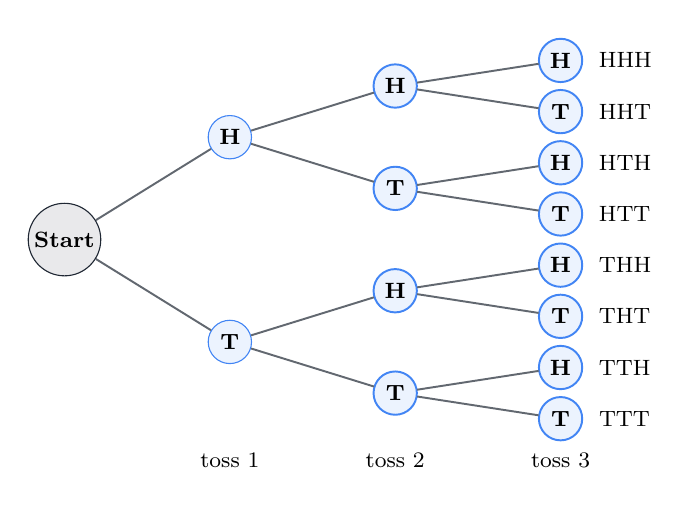
\begin{tikzpicture}[font=\sffamily\small,grow'=right,level distance=2.1cm,
  every node/.style={circle,draw=tmBlue,fill=tmBlue!10,inner sep=1.5pt,minimum size=0.55cm,font=\footnotesize\bfseries},
  level 1/.style={sibling distance=2.6cm},level 2/.style={sibling distance=1.3cm},level 3/.style={sibling distance=0.65cm},
  edge from parent/.style={draw=Ink!70,line width=0.7pt}]
\node[fill=Ink!10,draw=Ink] {Start}
  child {node {H}
    child {node {H} child {node {H}} child {node {T}}}
    child {node {T} child {node {H}} child {node {T}}}}
  child {node {T}
    child {node {H} child {node {H}} child {node {T}}}
    child {node {T} child {node {H}} child {node {T}}}};
\foreach \y/\t in {2.275/HHH,1.625/HHT,0.975/HTH,0.325/HTT,-0.325/THH,-0.975/THT,-1.625/TTH,-2.275/TTT}{
  \node[draw=none,fill=none,font=\footnotesize,anchor=west] at (6.7,\y) {\t};}
\node[draw=none,fill=none,font=\footnotesize] at (2.1,-2.8) {toss 1};
\node[draw=none,fill=none,font=\footnotesize] at (4.2,-2.8) {toss 2};
\node[draw=none,fill=none,font=\footnotesize] at (6.3,-2.8) {toss 3};
\end{tikzpicture}\end{center}
Example: the event ``exactly two heads'' consists of HHT, HTH, THH -- $3$ outcomes, so its probability is $\dfrac38$.

\begin{tipbox}
A problem like ``walk on a grid by tossing a coin'' (heads: move up, tails: move right) is really a problem about counting sequences of heads and tails: after $4$ tosses there are $2^4=16$ equally likely sequences, and the \emph{end point} depends only on the \emph{number of heads}, not on their order.
\end{tipbox}

% ----------------------------------------------------------------------
\shead{The multiplication rule and the addition rule}
\begin{knowbox}
\textbf{Multiplication rule.} If a task consists of two successive stages, stage 1 can be done in $m$ ways, and \emph{for each} way of doing stage 1, stage 2 can be done in $n$ ways, then the whole task can be done in $m\times n$ ways. (With three or four stages: keep multiplying.)

\medskip
\textbf{Addition rule (splitting into cases).} If the ways are split into cases that \emph{do not overlap}: case 1 has $a$ ways, case 2 has $b$ ways, \ldots, then the total number of ways is $a+b+\dots$

\medskip
\textbf{Common situations with digits.}
\begin{itemize}[leftmargin=1.2em,itemsep=1pt,topsep=2pt]
\item Three-digit numbers made from $3$ given non-zero digits, \emph{no repetition}: $3\times2\times1=6$ numbers.
\item Three-digit numbers made from $3$ given non-zero digits, \emph{repetition allowed}: $3\times3\times3=27$ numbers.
\item The first (leading) digit \textbf{cannot be $0$}: $9$ choices ($1$ to $9$); the other places have $10$ choices ($0$ to $9$).
\item A three-digit \textbf{palindrome} (reads the same forwards and backwards) has the form $\overline{aba}$: $9$ ways to choose $a$, $10$ ways to choose $b$, and the last digit is ``forced'' to equal $a$ (only $1$ way). There are $9\times10=90$ such numbers.
\end{itemize}
\end{knowbox}

\countboxes{hundreds/9/from 1 to 9/tmBlue,tens/10/from 0 to 9/tmOrange,ones/1/same as hundreds/tmGreen}{90}
\vspace{-6pt}
\begin{center}\footnotesize Number of three-digit palindromes: $9\times 10\times 1=90$.\end{center}

\begin{proofbox}
Why is the multiplication rule true? Draw a table with $m$ rows (the ways of doing stage 1) and $n$ columns (the ways of doing stage 2). Each cell of the table is \emph{exactly one} way of doing the whole task, and each way of doing the whole task is in \emph{exactly one} cell. The table has $m$ rows of $n$ cells, so $m\times n$ cells. A tree diagram gives the same result: $m$ big branches, each splitting into $n$ small branches.
\end{proofbox}

\begin{knowbox}
\textbf{Choosing two objects (order does not matter).} Choosing $2$ of $n$ students for classroom duty: if we care about order (first person, second person) there are $n\times(n-1)$ ways; but each pair is counted \emph{twice} (An--Bình and Bình--An), so the number of pairs is
\[
\frac{n\times(n-1)}{2}.
\]
Example: there are $\dfrac{10\times9}{2}=45$ pairs of different numbers taken from $10$ numbers.
\end{knowbox}

\begin{warnbox}
\textbf{Double counting.} When the question asks ``how many \emph{pairs}'', ``how many \emph{groups}'' (who comes first does not matter) and you use the multiplication rule with order, each group is counted several times -- you must divide. On the other hand, when the question is about \emph{numbers} (the order of the digits matters) or \emph{seating in a row}, order matters and you do \emph{not} divide.
\end{warnbox}

\begin{tipbox}
When splitting into cases, ask: ``Do the cases \emph{cover} every possibility? Do they \emph{overlap}?'' For example, for the sum $m+n$ to be even, $m$ and $n$ must be \emph{both odd} or \emph{both even} -- these two cases are separate and together they cover every possibility.
\end{tipbox}

% ----------------------------------------------------------------------
\shead{Reasoning by elimination: seating and colouring}
\begin{knowbox}
Some problems do not ask ``how many'' but ``\emph{who can}, \emph{who cannot}'', ``\emph{what is the least number needed}''. Then we use \textbf{reasoning}:
\begin{itemize}[leftmargin=1.2em,itemsep=1pt,topsep=2pt]
\item \textbf{Draw a diagram} of the positions (seats, cells, faces\ldots) and try filling it in.
\item Two people who \textbf{must sit together} can be treated as \textbf{one block} taking two neighbouring seats.
\item To show ``\emph{X can} sit in the middle seat'': just \textbf{give one arrangement} that satisfies all the conditions.
\item To show ``\emph{X cannot} sit in the middle seat'': \textbf{suppose} X sits in the middle seat and show that \emph{every} remaining arrangement breaks a condition (leading to a contradiction). This is called \textbf{proof by contradiction}.
\item A ``what is the \emph{least} number'' problem has \textbf{two parts}: (1) show a way that works with that number; (2) explain why fewer is impossible.
\end{itemize}
\end{knowbox}

\begin{figC}
\foreach \i in {1,...,5}{\draw[tmBlue,line width=1pt,fill=tmBlue!8,rounded corners=3pt] (\i*1.3-0.5,0) rectangle (\i*1.3+0.5,0.7);
  \node[font=\footnotesize] at (\i*1.3,-0.3){seat \i};}
\draw[tmOrange,line width=1.4pt,rounded corners=5pt] (3*1.3-0.62,-0.12) rectangle (3*1.3+0.62,0.82);
\node[font=\footnotesize\bfseries,text=tmOrange!80!black] at (3*1.3,1.1){middle seat};
\draw[decorate,decoration={brace,amplitude=5pt,mirror},Ink] (1*1.3-0.5,-0.55)--(2*1.3+0.5,-0.55) node[midway,below=5pt,font=\footnotesize]{two seats on the left};
\draw[decorate,decoration={brace,amplitude=5pt,mirror},Ink] (4*1.3-0.5,-0.55)--(5*1.3+0.5,-0.55) node[midway,below=5pt,font=\footnotesize]{two seats on the right};
\end{figC}
Key observation: once someone sits in the middle seat, the other four seats split into \emph{two pairs of neighbouring seats} (seats 1--2 and seats 4--5). The two seats on either side of the middle seat (seat 2 and seat 4) are \emph{not} next to each other.

\begin{knowbox}
\textbf{Colouring so that neighbouring parts have different colours.} Two faces of a cube are ``neighbours'' if they share an edge. Each face is a neighbour of $4$ faces and is \emph{not} a neighbour of exactly $1$ face -- the \textbf{opposite} face. A cube has $3$ pairs of opposite faces (top--bottom, front--back, left--right).
\begin{itemize}[leftmargin=1.2em,itemsep=1pt,topsep=2pt]
\item \emph{$3$ colours are enough:} paint each pair of opposite faces one colour; two faces of the same colour are opposite, so they are not neighbours.
\item \emph{Fewer than $3$ colours is impossible:} the three faces meeting at a corner are neighbours of each other in pairs, so they need three different colours.
\end{itemize}
\end{knowbox}

\begin{tipbox}
For a multiple-choice question ``Who \emph{cannot}\ldots?'', you can work backwards: for each option, try to find \emph{one} valid arrangement. Every option for which you find an arrangement is eliminated; the remaining option is the answer -- but remember to explain why it really cannot be arranged.
\end{tipbox}

% ----------------------------------------------------------------------
\shead{Counting shapes in a figure}
\begin{knowbox}
\textbf{Principle.} Counting shapes is a listing problem. To miss nothing and count nothing twice, \textbf{split into types} (by size, by position) and then \textbf{add up}.

\medskip
\textbf{The ``choose two lines'' trick.} A rectangle in a grid is completely determined by \emph{two horizontal lines} (top and bottom sides) and \emph{two vertical lines} (left and right sides). Therefore:
\begin{itemize}[leftmargin=1.2em,itemsep=1pt,topsep=2pt]
\item A strip of $1$ row and $n$ squares has $n+1$ vertical lines; the number of rectangles is the number of ways to choose $2$ vertical lines:
$\dfrac{(n+1)\times n}{2}$. Example: a strip of $4$ squares has $\dfrac{5\times4}{2}=10$ rectangles.
\item A grid with $a$ horizontal lines and $b$ vertical lines (all running the full length) has
$\dfrac{a(a-1)}{2}\times\dfrac{b(b-1)}{2}$ rectangles (multiplication rule!).
\item The same counting works for \emph{parallelograms} in a grid whose slanted lines are parallel to each other.
\end{itemize}
\end{knowbox}

\begin{figC}
\begin{scope}
\foreach \i in {0,...,4}{\draw[Ink,line width=1pt] (\i,0)--(\i,1); \node[font=\footnotesize,text=tmBlue] at (\i,-0.3){\pgfmathtruncatemacro\k{\i+1}\k};}
\draw[Ink,line width=1pt] (0,0)--(4,0) (0,1)--(4,1);
\fill[tmOrange,opacity=0.3] (1,0) rectangle (3,1);
\node[font=\footnotesize,align=center] at (2,-0.95){Choose vertical lines $2$ and $4$\\ $\Rightarrow$ the orange rectangle};
\end{scope}
\begin{scope}[xshift=6cm]
\foreach \x in {0,1,2,3}{\draw[Ink,line width=1pt] (\x,0)--(\x,2);}
\foreach \y in {0,1,2}{\draw[Ink,line width=1pt] (0,\y)--(3,\y);}
\fill[tmGreen,opacity=0.3] (1,0) rectangle (3,2);
\node[font=\footnotesize,align=center] at (1.5,-0.7){$3$ horizontal, $4$ vertical lines:\\ $3\times 6=18$ rectangles};
\end{scope}
\end{figC}

\begin{proofbox}
Why does a strip of $n$ squares have $\dfrac{(n+1)\times n}{2}$ rectangles? Choose the left side: $n+1$ ways; choose the right side (different from the left side): $n$ ways -- that gives $(n+1)\times n$ \emph{ordered} choices. But choosing ``line 2 then line 4'' or ``line 4 then line 2'' gives the same rectangle, so each rectangle is counted $2$ times; divide by $2$. Counting by size gives the same result: a strip of $4$ squares has $4$ rectangles of width $1$, $3$ of width $2$, $2$ of width $3$ and $1$ of width $4$, in total $4+3+2+1=10$.
\end{proofbox}

\begin{warnbox}
When the shapes \textbf{partly overlap} (not a grid with full-length lines), the ``choose two lines'' trick \emph{does not work}, because many segments do not run all the way across. Check each shape: \textbf{are all four sides really drawn?} Do not count ``imaginary rectangles'' that are missing a side.
\end{warnbox}

\begin{knowbox}
\textbf{Counting in a tiling.} A tiling made of regular octagons and small squares: if there are $m$ rows with $n$ octagons in each row, there are $m\times n$ octagons. Each small square sits where \emph{four octagons meet}; between $n$ columns there are $n-1$ gaps and between $m$ rows there are $m-1$ gaps, so there are $(m-1)\times(n-1)$ squares.
\end{knowbox}
\begin{figC}
\foreach \i in {0,1,2}{\foreach \j in {0,1}{\cpOct{\i}{\j}}}
\foreach \i in {0.5,1.5}{\cpDia{\i}{0.5}}
\node[font=\footnotesize,align=left,anchor=west] at (3,0.5){$2$ rows, $3$ columns: $2\times3=6$ octagons,\\ $(2-1)\times(3-1)=2$ squares.};
\end{figC}

% ----------------------------------------------------------------------
\shead{Counting with patterns: evenly spaced sequences, constant rates}
\begin{knowbox}
\textbf{Counting the whole numbers from $a$ to $b$} (including $a$ and $b$): there are $b-a+1$ numbers. For example from $1$ to $11$ there are $11$ numbers, of which $6$ are odd ($1,3,5,7,9,11$) and $5$ are even.

\medskip
\textbf{Evenly spaced sequence} (each number is a fixed amount $d$ more than the one before):
\[
\text{number of terms}=\frac{\text{last}-\text{first}}{d}+1,\qquad
\text{sum}=\frac{(\text{first}+\text{last})\times\text{number of terms}}{2}.
\]

\textbf{Quantities that change at a constant rate} (moving steadily, flowing steadily, counting steadily\ldots):
$\text{amount}=\text{rate}\times\text{time}$. For example, if $3$ sheep pass each minute, then in $14$ minutes $3\times14=42$ sheep pass.

\medskip
\textbf{Figures made of sticks.} Count the \emph{horizontal sticks} and the \emph{vertical sticks} separately and then add -- usually easier than counting square by square.

\medskip
\textbf{Events that repeat in cycles.} If one thing repeats every $a$ minutes and another every $b$ minutes, and they start together, they coincide again every $\text{LCM}(a,b)$ minutes.
\end{knowbox}

\begin{proofbox}
\textbf{Gauss's way of adding.} Compute $S=1+2+3+\dots+10$. Write the sum twice, once forwards and once backwards:
\[
\begin{array}{rcccccc}
S&=&1&+\;2&+\;3&+\dots+&10\\
S&=&10&+\;9&+\;8&+\dots+&1\\ \hline
2S&=&11&+\;11&+\;11&+\dots+&11
\end{array}
\]
There are $10$ columns, each with sum $11$, so $2S=10\times11=110$ and $S=55$. In general: sum $=\dfrac{(\text{first}+\text{last})\times\text{number of terms}}{2}$.
\end{proofbox}

\begin{warnbox}
\textbf{The ``off by one'' error.} From $3$ to $10$ there are $10-3+1=8$ numbers, \emph{not} $7$. A fence $10$ m long with a post every $1$ m (including both ends) needs $11$ posts, not $10$. Test a formula on a small example to check it.
\end{warnbox}

\begin{parentbox}
For ``toothpick'' problems, let your child actually build the small figures ($1$ square, $2$ squares, $3$ squares\ldots) with toothpicks, write the number of toothpicks in a table, and then ask: ``each time we add one square, how many toothpicks do we add?''. A child who finds the pattern alone remembers it much longer than a memorised formula.
\end{parentbox}

\begin{knowbox}
\textbf{Summary: read the clues, choose the tool.}\par\smallskip
\begin{tabularx}{\linewidth}{@{}>{\raggedright\arraybackslash}X>{\raggedright\arraybackslash}X@{}}
\textbf{Clue in the problem} & \textbf{Tool to use}\\ \hline
``choose one at random'', ``what is the probability'' & count all outcomes and favourable outcomes, then divide\\
probability given, quantity asked & favourable $=P\times$ total\\
something was taken out/eaten before the next draw & recount numerator and denominator\\
``at least one'', ``not'' & complement: $1-P$\\
two dice, two independent choices & two-way table\\
tossing a coin several times, several stages in a row & tree diagram\\
``how many numbers can be made'', ``how many ways'' & multiplication rule (choose restricted positions first)\\
``how many pairs'' (order does not matter) & multiplication rule, then divide by $2$\\
conditions of the form ``either\ldots or\ldots'' & split into cases, add\\
``who can / cannot'' & try one arrangement / proof by contradiction\\
``how many shapes\ldots'' & split by size, or choose two lines\\
rows of seats, toothpicks, constant rates & find the pattern, evenly spaced sequences\\
\end{tabularx}
\end{knowbox}

% ======================================================================
% EXAMPLES
% ======================================================================
\begin{exbox}{Example 1}
A box contains $3$ red marbles, $5$ blue marbles and $4$ yellow marbles, all of the same size. One marble is drawn at random.
\begin{enumerate}[label=\alph*),leftmargin=1.5em,itemsep=0pt,topsep=2pt]
\item Find the probability of drawing a blue marble.
\item Find the probability of drawing a marble that is \emph{not} red.
\item Find the probability of drawing a purple marble.
\end{enumerate}
\guide
\step{1}{Count all possible outcomes}
Each marble is one outcome, and since the marbles have the same size the outcomes are equally likely. Total number of marbles: $3+5+4=12$. So there are $12$ possible outcomes.
\step{2}{Part a}
There are $5$ blue marbles, i.e.\ $5$ favourable outcomes.
$P(\text{blue})=\dfrac{5}{12}$.
\step{3}{Part b -- use the complement}
$P(\text{red})=\dfrac{3}{12}=\dfrac14$, so $P(\text{not red})=1-\dfrac14=\dfrac34$.

\emph{Another way (direct counting):} the marbles that are not red are $5$ blue and $4$ yellow, i.e.\ $9$ marbles; $P=\dfrac{9}{12}=\dfrac34$. Both ways give the same result.
\step{4}{Part c}
There are no purple marbles in the box: $0$ favourable outcomes. $P(\text{purple})=\dfrac{0}{12}=0$ -- an impossible event.
\ans{a) $\frac{5}{12}$;\quad b) $\frac34$;\quad c) $0$.}
\end{exbox}

\begin{exbox}{Example 2}
A bag contains $30$ sweets, some strawberry and some orange. If one sweet is drawn at random, the probability that it is strawberry is $\dfrac25$.
\begin{enumerate}[label=\alph*),leftmargin=1.5em,itemsep=0pt,topsep=2pt]
\item How many strawberry sweets and how many orange sweets are in the bag?
\item An takes out $2$ strawberry sweets and eats them. Then Bình draws one sweet at random from the bag. Find the probability that Bình gets a strawberry sweet.
\end{enumerate}
\guide
\step{1}{Find the number of strawberry sweets}
\begin{recallbox}Number of favourable outcomes $=$ probability $\times$ number of all outcomes.\end{recallbox}
Strawberry sweets: $30\times\dfrac25=\dfrac{30\times 2}{5}=\dfrac{60}{5}=12$. Orange sweets: $30-12=18$.

\emph{Check:} $\dfrac{12}{30}=\dfrac{2}{5}$ \checkmark.
\step{2}{Recount after An eats $2$ sweets}
\begin{center}
\begin{tabular}{|l|c|c|c|}\hline
 & strawberry & orange & total \\ \hline
At the start & $12$ & $18$ & $30$\\ \hline
After An eats $2$ strawberry & $12-2=10$ & $18$ & $30-2=28$\\ \hline
\end{tabular}
\end{center}
\step{3}{Compute the probability for Bình}
$P(\text{strawberry})=\dfrac{10}{28}=\dfrac{5}{14}$.
\begin{warnbox}Do not answer $\dfrac{10}{30}$: An has eaten $2$ sweets, so the total number of sweets (the denominator) has gone down too.\end{warnbox}
\ans{a) $12$ strawberry, $18$ orange;\quad b) $\frac{5}{14}$.}
\end{exbox}

\begin{exbox}{Example 3}
A red die and a blue die (both fair) are rolled together. Find the probability of each event:
\begin{enumerate}[label=\alph*),leftmargin=1.5em,itemsep=0pt,topsep=2pt]
\item The sum of the two numbers is $8$.
\item Both dice show the same number.
\item The sum of the two numbers is greater than or equal to $10$.
\end{enumerate}
\guide
\step{1}{Make a table of all outcomes}
Rows are the numbers on the red die, columns the numbers on the blue die, and each cell shows the sum. The table has $6\times6=36$ cells, corresponding to $36$ equally likely outcomes.
\begin{figC}
\foreach \c in {1,...,6}{\node[draw=tmBlue,fill=tmBlue!15,minimum size=0.6cm,font=\bfseries] at (\c*0.6,0.4) {\c};}
\foreach \r in {1,...,6}{\node[draw=AnsRed,fill=AnsRed!12,minimum size=0.6cm,font=\bfseries] at (0,0.4-\r*0.6) {\r};
  \foreach \c in {1,...,6}{\pgfmathtruncatemacro\s{\r+\c}%
    \def\fc{white}%
    \ifnum\s=8 \def\fc{tmOrange!40}\fi
    \ifnum\s>9 \def\fc{tmGreen!30}\fi
    \node[draw=Line,fill=\fc,minimum size=0.6cm] at (\c*0.6,0.4-\r*0.6) {\s};
    \ifnum\r=\c \draw[tmPurple,line width=1pt] (\c*0.6,0.4-\r*0.6) circle (0.24);\fi}}
\node[font=\footnotesize,align=left,anchor=west] at (4.4,-1.7) {\colorbox{tmOrange!40}{\strut\ \ } sum equals $8$ ($5$ cells)\\[2pt]
  {\color{tmPurple}$\bigcirc$} both numbers equal ($6$ cells)\\[2pt] \colorbox{tmGreen!30}{\strut\ \ } sum $\ge 10$ ($6$ cells)};
\end{figC}
\step{2}{Part a}
The cells with sum $8$: $(2,6),(3,5),(4,4),(5,3),(6,2)$ -- $5$ outcomes (the first number is the red die). $P=\dfrac{5}{36}$.
\step{3}{Part b}
Equal numbers lie on the diagonal: $(1,1),(2,2),\dots,(6,6)$ -- $6$ outcomes. $P=\dfrac{6}{36}=\dfrac16$.
\step{4}{Part c}
Sum $10$: $(4,6),(5,5),(6,4)$; sum $11$: $(5,6),(6,5)$; sum $12$: $(6,6)$. Altogether $3+2+1=6$ outcomes. $P=\dfrac{6}{36}=\dfrac16$.
\begin{tipbox}The $6\times6$ table also shows \emph{symmetry}: the number of cells above the diagonal (red smaller than blue) equals the number of cells below the diagonal (red greater than blue).\end{tipbox}
\ans{a) $\frac{5}{36}$;\quad b) $\frac16$;\quad c) $\frac16$.}
\end{exbox}

\begin{exbox}{Example 4}
A fair coin is tossed three times in a row. Find the probability of getting:
a) exactly two heads;\quad b) at least one head.
\guide
\step{1}{Draw a tree diagram and list}
Each toss has $2$ outcomes (H or T). By the tree diagram in section 3, there are $2\times2\times2=8$ equally likely outcomes:
\[
\text{HHH},\ \text{HHT},\ \text{HTH},\ \text{HTT},\ \text{THH},\ \text{THT},\ \text{TTH},\ \text{TTT}.
\]
\step{2}{Part a}
The outcomes with exactly two H's: HHT, HTH, THH -- $3$ outcomes. $P=\dfrac38$.
\step{3}{Part b -- complement}
The complement of ``at least one head'' is ``no heads at all'', which is only TTT ($1$ outcome). So
$P(\text{at least one H})=1-\dfrac18=\dfrac78$.
\begin{tipbox}When you see the words ``\emph{at least one}'', think immediately of the complement ``\emph{none at all}'' -- it usually has very few outcomes and is easy to count.\end{tipbox}
\ans{a) $\frac38$;\quad b) $\frac78$.}
\end{exbox}

\begin{exbox}{Example 5}
Using the digits $1,2,3,4$, how many three-digit numbers can be made if:
a) digits may be repeated;\quad b) the digits must be different;\quad c) the digits are different and the number is even?\\
d) One of the numbers from part b) is chosen at random. Find the probability that it is even.
\guide
\step{1}{Part a -- repetition allowed}
Hundreds: $4$ ways; tens: still $4$ ways; ones: $4$ ways. By the multiplication rule: $4\times4\times4=64$ numbers.
\step{2}{Part b -- no repetition}
\countboxes{hundreds/4/any/tmBlue,tens/3/not the hundreds digit/tmOrange,ones/2/not the two above/tmGreen}{24}
Hundreds: $4$ ways. The tens digit must differ from the digit already used: $3$ ways. The ones digit must differ from both digits used: $2$ ways. There are $4\times3\times2=24$ numbers.
\step{3}{Part c -- even, no repetition: choose the ones digit FIRST}
An even number ends in $2$ or $4$: $2$ ways. Then the hundreds digit is one of the $3$ remaining digits: $3$ ways; the tens digit: $2$ ways. There are $2\times3\times2=12$ numbers.
\begin{tipbox}A position with a \emph{condition} (must be even, must not be $0$\ldots) should be \textbf{chosen first}. If you choose the hundreds digit first, the number of choices for the ones digit is sometimes $1$ and sometimes $2$ (depending on whether the hundreds digit used an even or an odd digit) -- very easy to get wrong.\end{tipbox}
\step{4}{Part d}
$P(\text{even})=\dfrac{12}{24}=\dfrac12$.
\verify{List the numbers starting with $1$: $123,124,132,134,142,143$ -- exactly $6=3\times2$ numbers, of which $124,132,134,142$ are even ($4$ numbers). The four possible first digits behave alike, so there are $4\times6=24$ numbers, \ldots\ matching part b.}
\ans{a) $64$;\quad b) $24$;\quad c) $12$;\quad d) $\frac12$.}
\end{exbox}

\begin{exbox}{Example 6}
Four friends An, Bình, Chi and Dũng sit on four chairs in a row, numbered $1,2,3,4$ from left to right. We know that: Dũng sits on chair $1$; Bình and Chi sit next to each other; An does not sit next to Bình; An does not sit on chair $4$. Who sits on chair $4$?
\guide
\step{1}{Place Dũng}
Dũng is on chair $1$, leaving chairs $2,3,4$ for An, Bình and Chi.
\step{2}{Consider An's position}
An does not sit on chair $4$, so An sits on chair $2$ or chair $3$.
\begin{itemize}[leftmargin=1.2em,itemsep=1pt,topsep=1pt]
\item \emph{If An sits on chair $3$:} Bình and Chi take chairs $2$ and $4$ -- these chairs are not next to each other, which breaks the condition ``Bình and Chi sit next to each other''. Rejected.
\item \emph{If An sits on chair $2$:} Bình and Chi take chairs $3$ and $4$ (next to each other, good). An must not be next to Bình, and chair $3$ is next to chair $2$, so Bình is not on chair $3$. So Bình is on chair $4$ and Chi on chair $3$.
\end{itemize}
\begin{figC}
\foreach \i/\n/\c in {1/Dũng/tmPurple,2/An/tmOrange,3/Chi/tmGreen,4/Bình/tmBlue}{
  \draw[\c,line width=1pt,fill=\c!12,rounded corners=3pt] (\i*1.6-0.65,0) rectangle (\i*1.6+0.65,0.7);
  \node[font=\bfseries] at (\i*1.6,0.35){\n};\node[font=\footnotesize] at (\i*1.6,-0.3){chair \i};}
\end{figC}
\verify{Dũng on chair $1$ \checkmark; Bình (chair $4$) next to Chi (chair $3$) \checkmark; An (chair $2$) is next to Dũng and Chi, not next to Bình \checkmark; An is not on chair $4$ \checkmark.}
\ans{Bình sits on chair $4$.}
\end{exbox}

\begin{exbox}{Example 7}
a) The figure on the left is a strip of $4$ squares. How many rectangles (including squares) are there altogether?\\
b) The figure on the right is a $2\times2$ grid of squares. How many rectangles are there? How many of them are squares?
\begin{figC}
\foreach \i in {0,...,4}{\draw[Ink,line width=1pt] (\i*0.8,0)--(\i*0.8,0.8);}
\draw[Ink,line width=1pt] (0,0)--(3.2,0) (0,0.8)--(3.2,0.8);
\begin{scope}[xshift=5.5cm]
\foreach \i in {0,1,2}{\draw[Ink,line width=1pt] (\i*0.8,0)--(\i*0.8,1.6) (0,\i*0.8)--(1.6,\i*0.8);}
\end{scope}
\end{figC}
\guide
\step{1}{Part a -- count by width}
Measure the width in squares:
\begin{center}
\begin{tabular}{|c|c|c|c|c|}\hline
Width & $1$ square & $2$ squares & $3$ squares & $4$ squares\\ \hline
Number of shapes & $4$ & $3$ & $2$ & $1$\\ \hline
\end{tabular}
\end{center}
Total: $4+3+2+1=10$ rectangles. \emph{Check with the ``choose two vertical lines'' trick:} there are $5$ vertical lines, and the number of ways to choose $2$ of them is $\dfrac{5\times4}{2}=10$ \checkmark.
\step{2}{Part b -- choose two horizontal and two vertical lines}
The grid has $3$ horizontal and $3$ vertical lines. Choose $2$ horizontal lines: $\dfrac{3\times2}{2}=3$ ways; choose $2$ vertical lines: $3$ ways. By the multiplication rule there are $3\times3=9$ rectangles.
\step{3}{Count the squares separately}
$1\times1$ squares: $4$; $2\times2$ squares: $1$ (the whole grid). There are $4+1=5$ squares.
\verify{Counting by size: $1\times1$: $4$; $1\times2$ (lying flat): $2$; $2\times1$ (standing): $2$; $2\times2$: $1$. Total $4+2+2+1=9$ \checkmark.}
\ans{a) $10$ rectangles;\quad b) $9$ rectangles, of which $5$ are squares.}
\end{exbox}

\begin{exbox}{Example 8}
Toothpicks are used to make a row of joined squares as shown below.
\begin{figC}
\foreach \n/\x in {1/0,2/2,3/5}{
  \foreach \i in {0,...,\n}{\draw[tmOrange!80!black,line width=1.6pt,line cap=round] (\x+\i*0.7,0.05)--(\x+\i*0.7,0.65);}
  \foreach \i in {1,...,\n}{\draw[tmOrange!80!black,line width=1.6pt,line cap=round] (\x+\i*0.7-0.65,0)--(\x+\i*0.7-0.05,0) (\x+\i*0.7-0.65,0.7)--(\x+\i*0.7-0.05,0.7);}
  \node[font=\footnotesize] at (\x+\n*0.35,-0.35){\n\ sq.};}
\end{figC}
a) How many toothpicks are needed for a row of $20$ squares?\\
b) Lan builds, one after another and separately, a row of $1$ square, a row of $2$ squares, \ldots, a row of $10$ squares. How many toothpicks does Lan use altogether?
\guide
\step{1}{Find the pattern}
\begin{center}
\begin{tabular}{|c|c|c|c|c|}\hline
Squares & $1$ & $2$ & $3$ & $n$\\ \hline
Toothpicks & $4$ & $7$ & $10$ & $3n+1$\\ \hline
\end{tabular}
\end{center}
Explanation: count each kind of toothpick separately. Horizontal toothpicks: each square has $1$ on top and $1$ at the bottom, that is $2n$ toothpicks. Vertical toothpicks: $n$ squares have $n+1$ vertical toothpicks (just as $n$ gaps need $n+1$ posts). Total $2n+(n+1)=3n+1$.
\step{2}{Part a}
$n=20$: $3\times20+1=61$ toothpicks.
\step{3}{Part b -- sum of an evenly spaced sequence}
The numbers of toothpicks are $4,7,10,\dots,31$ (a row of $10$ squares needs $3\times10+1=31$ toothpicks). This is an evenly spaced sequence with step $3$ and $10$ terms.
\begin{recallbox}Sum of an evenly spaced sequence $=\dfrac{(\text{first}+\text{last})\times\text{number of terms}}{2}$.\end{recallbox}
Sum: $\dfrac{(4+31)\times10}{2}=\dfrac{350}{2}=175$ toothpicks.
\verify{$4+7+10+13+16+19+22+25+28+31$: pair first with last, $4+31=7+28=10+25=13+22=16+19=35$, giving $5$ pairs, $5\times35=175$ \checkmark.}
\ans{a) $61$ toothpicks;\quad b) $175$ toothpicks.}
\end{exbox}

% ======================================================================
\clearpage
\dividerbar{Core practice}

% ---------------------------------------------------------------- Problem 1
\begin{probbox}{1}{\relax}
\begin{minipage}[t]{0.66\linewidth}\vspace{0pt}
The spinner shown is divided into $6$ sectors of equal size, each marked with a letter. The spinner is spun once. What is the probability that the arrow lands on a sector marked with the letter $P$?
\choices{$\dfrac{3}{6}$}{$\dfrac{4}{6}$}{$\dfrac{5}{6}$}{$\dfrac{2}{6}$}{$\dfrac{1}{6}$}
\end{minipage}\hfill
\begin{minipage}[t]{0.3\linewidth}\vspace{0pt}
\centering\begin{tikzpicture}[scale=0.95]\cpSpinSix{P}{R}{P}{Q}{R}{Q}\end{tikzpicture}
\end{minipage}
\end{probbox}
\probsol{
\textbf{Understanding the problem.} The spinner has $6$ \emph{equal} sectors, so when it is spun the arrow is equally likely to stop in each sector. We need the probability that the arrow points to a sector marked $P$.
\begin{recallbox}When the outcomes are equally likely: $P(\text{event})=\dfrac{\text{number of favourable outcomes}}{\text{number of all outcomes}}$.\end{recallbox}
\step{1}{Count all possible outcomes}
The arrow can stop in any one of the $6$ sectors, so there are $6$ possible outcomes.
\step{2}{Count the favourable outcomes}
Reading the letters clockwise, starting from the top-left sector: $P,\ R,\ P,\ Q,\ R,\ Q$. Exactly $2$ sectors are marked $P$ (the top-left one and the right one).
\step{3}{Compute the probability}
$P(\text{letter }P)=\dfrac{2}{6}$ $\left(=\dfrac13\right)$.
\begin{warnbox}There are $3$ different letters ($P$, $Q$, $R$), but the probability is \emph{not} computed as ``$1$ letter out of $3$ letters''. Here $\dfrac13=\dfrac26$ only by coincidence, because each letter appears exactly $2$ times; if the letters took up different numbers of sectors, that way of thinking would be wrong. Always count \emph{sectors}, not \emph{kinds of letters}.\end{warnbox}
\verify{Each of the letters $P$, $Q$, $R$ takes $2$ sectors: $\dfrac26+\dfrac26+\dfrac26=1$ -- the probabilities of all possibilities add up to $1$, as they should.}
The value $\dfrac26$ matches option \textbf{(D)}. (Option (A) $\dfrac36$ comes from miscounting $3$ sectors; (E) $\dfrac16$ is the probability of \emph{one} particular sector.)
\ans{(D) $\dfrac{2}{6}$}
}

% ---------------------------------------------------------------- Problem 2
\begin{probbox}{2}{\relax}
Using the three digits $4$, $7$ and $9$, each digit used \emph{at most once}, how many three-digit whole numbers with different digits can be made?
\choices{$6$}{$3$}{$5$}{$12$}{$9$}
\end{probbox}
\probsol{
\textbf{Understanding the problem.} A three-digit number using exactly the digits $4,7,9$, with no digit repeated. So each number is an \emph{arrangement} of these three digits in the three places: hundreds, tens, ones.
\step{1}{Method 1 -- systematic listing}
Order by the hundreds digit (from smallest to largest):
\begin{itemize}[leftmargin=1.2em,itemsep=0pt,topsep=1pt]
\item Hundreds digit $4$: the other two digits $7,9$ give $479$ and $497$.
\item Hundreds digit $7$: $749$ and $794$.
\item Hundreds digit $9$: $947$ and $974$.
\end{itemize}
There are $2+2+2=6$ numbers.
\step{2}{Method 2 -- multiplication rule}
\begin{recallbox}Multiplication rule: if a task has several successive stages, each with a number of ways (not depending on the choices made before), then the number of ways to do the whole task is the \emph{product} of those numbers.\end{recallbox}
\countboxes{hundreds/3/4 or 7 or 9/tmBlue,tens/2/2 digits left/tmOrange,ones/1/the last digit/tmGreen}{6}
Hundreds: $3$ choices. Tens: only $2$ unused digits remain, $2$ choices. Ones: exactly $1$ digit remains, $1$ choice. Number of numbers: $3\times2\times1=6$.
\begin{warnbox}If repeated digits were allowed there would be $3\times3\times3=27$ numbers (such as $444$, $477$\ldots). The problem forbids repetition, so after each stage the number of choices goes down by $1$.\end{warnbox}
\verify{The six numbers $479,497,749,794,947,974$ are all different and all use the three digits. Both methods give the same result.}
The answer $6$ is option \textbf{(A)}. (Option (B) $3$ is just the number of digits given.)
\ans{(A) $6$}
}

% ---------------------------------------------------------------- Problem 3
\begin{probbox}{3}{\relax}
An envelope contains $2$ sunflower seeds, $3$ mung bean seeds and $4$ pumpkin seeds. Chi takes one seed from the envelope at random. What is the probability that Chi takes a sunflower seed?
\choices{$\dfrac{2}{9}$}{$\dfrac{5}{9}$}{$\dfrac{9}{7}$}{$\dfrac{7}{9}$}{$\dfrac{1}{9}$}
\end{probbox}
\probsol{
\textbf{Understanding the problem.} The envelope has three kinds of seeds in different numbers. Chi takes \emph{one seed} at random: every seed has the same chance of being taken, so each \emph{seed} is one equally likely outcome.
\step{1}{Count all possible outcomes}
Total number of seeds: $2+3+4=9$, i.e.\ $9$ outcomes.
\step{2}{Count the favourable outcomes}
There are $2$ sunflower seeds, so $2$ favourable outcomes.
\step{3}{Compute the probability}
\begin{recallbox}$P=\dfrac{\text{number of favourable outcomes}}{\text{number of all outcomes}}$.\end{recallbox}
$P(\text{sunflower})=\dfrac{2}{9}$.
\begin{warnbox}There are $3$ \emph{kinds} of seeds but the answer is not $\dfrac13$, because the pumpkin seeds are more numerous and so more likely to be taken. Remember too that a probability is never greater than $1$, so option (C) $\dfrac97$ is certainly wrong.\end{warnbox}
\verify{$P(\text{sunflower})+P(\text{mung bean})+P(\text{pumpkin})=\dfrac29+\dfrac39+\dfrac49=\dfrac99=1$.}
The result $\dfrac29$ is option \textbf{(A)}. (Option (D) $\dfrac79$ is the probability of \emph{not} taking a sunflower seed.)
\ans{(A) $\dfrac{2}{9}$}
}

% ---------------------------------------------------------------- Problem 4
\begin{probbox}{4}{\relax}
A cinema has $11$ rows of seats, numbered from $1$ to $11$. Each odd-numbered row has $15$ seats and each even-numbered row has $16$ seats. How many seats are there in the cinema altogether?
\choices{$176$}{$186$}{$165$}{$170$}{$171$}
\end{probbox}
\probsol{
\textbf{Understanding the problem.} The number of seats in a row depends on whether the row number is odd or even. So we need to know how many of the numbers from $1$ to $11$ are odd and how many are even.
\step{1}{Count the odd rows and the even rows}
Odd rows: $1,3,5,7,9,11$ -- $6$ rows.\\
Even rows: $2,4,6,8,10$ -- $5$ rows.\\
Check: $6+5=11$ rows \checkmark.
\begin{figC}
\foreach \i in {1,...,11}{\pgfmathtruncatemacro\m{mod(\i,2)}%
  \ifnum\m=1 \def\cc{tmBlue}\else\def\cc{tmOrange}\fi
  \draw[\cc,line width=0.9pt,fill=\cc!15,rounded corners=2pt] (\i*0.75-0.33,0) rectangle (\i*0.75+0.33,0.55);
  \node[font=\footnotesize\bfseries] at (\i*0.75,0.275){\i};}
\node[font=\footnotesize,text=tmBlue!80!black,anchor=west] at (9,0.55){odd row: $15$ seats};
\node[font=\footnotesize,text=tmOrange!80!black,anchor=west] at (9,0.05){even row: $16$ seats};
\end{figC}
\begin{warnbox}Do not split the $11$ rows into ``$5.5$ odd rows and $5.5$ even rows''. The list starts \emph{and} ends with an odd number ($1$ and $11$), so there is exactly $1$ more odd number than even numbers.\end{warnbox}
\step{2}{Seats in the odd rows}
$6\times15=90$ seats.
\step{3}{Seats in the even rows}
$5\times16=80$ seats.
\step{4}{Add up}
Total number of seats: $90+80=170$.
\verify{\emph{Another way -- pairing:} pair row $1$ with row $2$, row $3$ with row $4$, \ldots, row $9$ with row $10$: that gives $5$ pairs, each with $15+16=31$ seats, i.e.\ $5\times31=155$ seats; row $11$ with $15$ seats is left over. Total $155+15=170$ \checkmark.}
The answer $170$ is option \textbf{(D)}. (Mixing up and taking $5$ odd rows and $6$ even rows gives $171$ -- option (E), a very common ``trap''.)
\ans{(D) $170$}
}

% ---------------------------------------------------------------- Problem 5
\begin{probbox}{5}{\relax}
At a class party, each student in turn draws a wrapped present at random from a bag. The presents are only books and calculators; there are $27$ presents in the bag altogether. Mai draws first. The probability that Mai draws a book is $\dfrac23$. How many books are in the bag?
\choices{$15$}{$9$}{$21$}{$7$}{$18$}
\end{probbox}
\probsol{
\textbf{Understanding the problem.} A ``backwards'' problem: we know the \emph{probability} and the \emph{total} number of presents, and need the \emph{number of favourable outcomes} (the number of books). Since Mai draws first, all $27$ presents are still in the bag.
\begin{recallbox}From $P=\dfrac{\text{number of favourable outcomes}}{\text{number of all outcomes}}$ we get: number of favourable outcomes $=P\times$ number of all outcomes.\end{recallbox}
\step{1}{Call the number of books an unknown}
Let the number of books be $s$. The probability of drawing a book is $\dfrac{s}{27}$. By the problem: $\dfrac{s}{27}=\dfrac23$.
\step{2}{Find $s$}
$s=27\times\dfrac23=\dfrac{27\times2}{3}=\dfrac{54}{3}=18$.

\emph{Thinking with a bar model:} $\dfrac23$ means splitting the $27$ presents into $3$ equal parts of $27\div3=9$ presents each; books take $2$ parts, i.e.\ $2\times 9=18$ books.
\begin{figC}
\blk{0}{3}{0}{0.6}{tmBlue}{9 books}\blk{3}{6}{0}{0.6}{tmBlue}{9 books}\blk{6}{9}{0}{0.6}{tmOrange}{9 calculators}
\brcup{0}{9}{0.5}{$27$ presents}
\brcdn{0}{6}{-0.5}{$\frac23$ are books: $18$ books}
\end{figC}
\verify{There are $18$ books and $27-18=9$ calculators. Probability of drawing a book: $\dfrac{18}{27}=\dfrac{18\div9}{27\div9}=\dfrac23$ \checkmark.}
\begin{warnbox}The $9$ in option (B) is the number of \emph{calculators}, not books -- read the question carefully before choosing.\end{warnbox}
The answer $18$ is option \textbf{(E)}.
\ans{(E) $18$}
}

% ---------------------------------------------------------------- Problem 6
\begin{probbox}{6}{\relax}
A crate of fruit contains $20$ apples, $10$ oranges and no other fruit. One fruit is taken from the crate at random. What is the probability that it is an orange?
\choices{$\dfrac{1}{10}$}{$\dfrac{1}{20}$}{$\dfrac{1}{30}$}{$\dfrac{1}{3}$}{$\dfrac{2}{3}$}
\end{probbox}
\probsol{
\textbf{Understanding the problem.} Every fruit in the crate has the same chance of being taken. A favourable outcome is taking one of the oranges.
\step{1}{Count all outcomes}
Total number of fruits: $20+10=30$.
\step{2}{Count the favourable outcomes}
There are $10$ oranges.
\step{3}{Compute and simplify}
\begin{recallbox}$P=\dfrac{\text{number of favourable outcomes}}{\text{number of all outcomes}}$; simplify a fraction by dividing the numerator and denominator by their GCD.\end{recallbox}
$P(\text{orange})=\dfrac{10}{30}=\dfrac{10\div10}{30\div10}=\dfrac13$.
\begin{warnbox}Two common mistakes: (1) using the number of apples ($20$) as the denominator instead of the \emph{total number of fruits} ($30$), giving $\dfrac{10}{20}$; (2) writing $\dfrac{1}{10}$ (option A) thinking ``there are $10$ oranges so each is $\dfrac1{10}$''. The denominator is always \emph{all} the outcomes.\end{warnbox}
\verify{$P(\text{apple})=\dfrac{20}{30}=\dfrac23$ and $\dfrac13+\dfrac23=1$ \checkmark. It also makes sense: there are twice as many apples as oranges, so an apple is twice as likely as an orange.}
The result $\dfrac13$ is option \textbf{(D)}. (Option (E) $\dfrac23$ is the probability of taking an apple.)
\ans{(D) $\dfrac13$}
}

% ---------------------------------------------------------------- Problem 7
\begin{probbox}{7}{\relax}
A bag contains $2$ red balls, $5$ yellow balls and $4$ blue balls, all the same size. Without looking, one ball is taken from the bag. The probability of taking a yellow ball is
\choices{$\dfrac{2}{11}$}{$\dfrac{5}{11}$}{$\dfrac{4}{11}$}{$\dfrac{6}{11}$}{$\dfrac{7}{11}$}
\end{probbox}
\probsol{
\textbf{Understanding the problem.} ``Without looking'' and ``the same size'' guarantee that every ball has the same chance of being taken.
\step{1}{Count all outcomes}
Total number of balls: $2+5+4=11$.
\step{2}{Count the favourable outcomes}
There are $5$ yellow balls.
\step{3}{Compute the probability}
\begin{recallbox}$P=\dfrac{\text{number of favourable outcomes}}{\text{number of all outcomes}}$.\end{recallbox}
$P(\text{yellow})=\dfrac{5}{11}$ (this fraction is already in lowest terms because $5$ and $11$ have no common factor other than $1$).
\begin{figC}
\foreach \i in {1,2}{\shade[ball color=AnsRed] (\i*0.6,0) circle (0.22);}
\foreach \i in {3,...,7}{\shade[ball color=tmOrange] (\i*0.6+0.3,0) circle (0.22);\draw[tmOrange!70!black,line width=0.8pt] (\i*0.6+0.3,0) circle (0.27);}
\foreach \i in {8,...,11}{\shade[ball color=tmBlue] (\i*0.6+0.6,0) circle (0.22);}
\node[font=\footnotesize] at (3.9,-0.55){$5$ of the $11$ balls are yellow};
\end{figC}
\verify{$\dfrac{2}{11}+\dfrac{5}{11}+\dfrac{4}{11}=\dfrac{11}{11}=1$ \checkmark.}
The distractors: (A) $\dfrac{2}{11}$ is the probability of red, (C) $\dfrac{4}{11}$ the probability of blue, (D) $\dfrac{6}{11}$ the probability of \emph{not} taking a yellow ball. The correct answer is \textbf{(B)}.
\ans{(B) $\dfrac{5}{11}$}
}

% ---------------------------------------------------------------- Problem 8
\begin{probbox}{8}{\relax}
You are doing a multiple-choice test. On one question you do not know the answer, so you choose an option at random. If the question has five options (A, B, C, D, E) and only one of them is correct, what is the probability that you guess correctly?
\choices{$\dfrac{1}{5}$}{$\dfrac{5}{5}$}{$\dfrac{4}{5}$}{$\dfrac{2}{5}$}{$\dfrac{3}{5}$}
\end{probbox}
\probsol{
\textbf{Understanding the problem.} ``Choose at random'' means the five options are equally likely to be chosen. The question has exactly \emph{one} correct option.
\step{1}{Count all outcomes}
There are $5$ options to choose from: A, B, C, D, E.
\step{2}{Count the favourable outcomes}
Only $1$ option is correct, so there is $1$ favourable outcome.
\step{3}{Compute the probability}
\begin{recallbox}$P=\dfrac{\text{number of favourable outcomes}}{\text{number of all outcomes}}$.\end{recallbox}
$P(\text{correct})=\dfrac15$.
\begin{tipbox}The probability of guessing \emph{wrong} is $1-\dfrac15=\dfrac45$ -- option (C). So when guessing you are $4$ times more likely to be wrong than right. And (B) $\dfrac55=1$ means ``certainly correct'' -- absurd for a guess.\end{tipbox}
\verify{If you did $100$ such questions and guessed every one, you would get about $100\times\dfrac15=20$ right on average -- matching the feeling ``$1$ right out of every $5$''.}
The answer is \textbf{(A)}.
\ans{(A) $\dfrac15$}
}

% ---------------------------------------------------------------- Problem 9
\begin{probbox}{9}{\relax}
A fair six-sided die has the numbers $1$ to $6$ on its faces. The die is rolled once. What is the probability that it shows a $5$?
\choices{$\dfrac{2}{6}$}{$\dfrac{1}{6}$}{$\dfrac{5}{6}$}{$\dfrac{3}{6}$}{$\dfrac{4}{6}$}
\end{probbox}
\probsol{
\textbf{Understanding the problem.} The die is \emph{fair}, so the six faces are equally likely. The event we care about: ``the face showing is $5$''.
\step{1}{List the possible outcomes}
$\{1,\,2,\,3,\,4,\,5,\,6\}$ -- $6$ equally likely outcomes.
\step{2}{Count the favourable outcomes}
Only one face shows $5$: $1$ favourable outcome.
\step{3}{Compute the probability}
\begin{recallbox}$P=\dfrac{\text{number of favourable outcomes}}{\text{number of all outcomes}}$.\end{recallbox}
$P(5)=\dfrac16$.
\begin{warnbox}Do not confuse ``the number $5$'' with ``the number of favourable outcomes''. Many students write $\dfrac56$ (option C) because they see a $5$ in the question. The $5$ is only the \emph{name} of the face; the number of faces with that name is only $1$. ($\dfrac56$ is the probability of rolling a number \emph{from $1$ to $5$}, i.e.\ anything but $6$.)\end{warnbox}
\verify{Each face has probability $\dfrac16$, and the six faces together give $\dfrac66=1$ \checkmark.}
The answer is \textbf{(B)}.
\ans{(B) $\dfrac16$}
}

% ---------------------------------------------------------------- Problem 10
\begin{probbox}{10}{\relax}
Five friends An, Hà, Chi, Minh and Tùng sit in a row of five seats. An does \emph{not} sit next to Hà, and Chi sits next to Minh. Who \emph{cannot} sit in the middle seat?
\choices{An}{Hà}{Chi}{Minh}{Tùng}
\end{probbox}
\probsol{
\textbf{Understanding the problem.} The five seats are in a row, numbered $1,2,3,4,5$ from left to right; the middle seat is seat $3$. Two conditions: (i) An and Hà do \emph{not} sit next to each other; (ii) Chi and Minh sit next to each other. We must find the friend who can \emph{never} sit in seat $3$.
\begin{recallbox}To show that a friend \emph{can} sit in the middle: just give \emph{one} arrangement satisfying every condition. To show that a friend \emph{cannot}: suppose they sit in the middle and show that every arrangement then breaks a condition (proof by contradiction).\end{recallbox}
\step{1}{An, Hà, Chi and Minh can each sit in the middle}
Here is one arrangement for each of them (seats $1\to5$):
\begin{center}
\begin{tabular}{|c|c|c|c|c|c|l|}\hline
In the middle & seat 1 & seat 2 & \textbf{seat 3} & seat 4 & seat 5 & check\\ \hline
An & Chi & Minh & \textbf{An} & Tùng & Hà & An (3), Hà (5) not neighbours\\ \hline
Hà & Chi & Minh & \textbf{Hà} & Tùng & An & Hà (3), An (5) not neighbours\\ \hline
Chi & An & Minh & \textbf{Chi} & Tùng & Hà & Chi (3) next to Minh (2)\\ \hline
Minh & An & Chi & \textbf{Minh} & Tùng & Hà & Minh (3) next to Chi (2)\\ \hline
\end{tabular}
\end{center}
In all four arrangements Chi and Minh are always neighbours, and An and Hà are always apart (An in seat $1$ or $3$, Hà in seat $5$, or the other way round). So options (A), (B), (C), (D) are eliminated.
\step{2}{Show that Tùng cannot sit in the middle}
Suppose Tùng sits in seat $3$. The other four seats split into two pairs of neighbouring seats: the left pair (seats $1$--$2$) and the right pair (seats $4$--$5$). Note that seats $2$ and $4$ are \emph{not} neighbours (Tùng is between them).
\begin{figC}
\foreach \i/\n/\c in {1/?/tmBlue,2/?/tmBlue,3/Tùng/tmOrange,4/?/tmGreen,5/?/tmGreen}{
  \draw[\c,line width=1pt,fill=\c!12,rounded corners=3pt] (\i*1.5-0.6,0) rectangle (\i*1.5+0.6,0.65);
  \node[font=\bfseries] at (\i*1.5,0.33){\n};\node[font=\footnotesize] at (\i*1.5,-0.28){seat \i};}
\draw[decorate,decoration={brace,amplitude=5pt,mirror},Ink] (0.9,-0.5)--(3.6,-0.5) node[midway,below=5pt,font=\footnotesize]{left pair};
\draw[decorate,decoration={brace,amplitude=5pt,mirror},Ink] (5.4,-0.5)--(8.1,-0.5) node[midway,below=5pt,font=\footnotesize]{right pair};
\end{figC}
\begin{itemize}[leftmargin=1.2em,itemsep=1pt,topsep=1pt]
\item Chi and Minh must be neighbours, and the only neighbouring seats (not counting Tùng's) are seats $1$--$2$ or seats $4$--$5$. So Chi and Minh take up one whole pair.
\item Then An and Hà are forced into the other pair -- that is, \emph{next to each other}. This contradicts the condition ``An does not sit next to Hà''.
\end{itemize}
So the assumption is false: Tùng cannot sit in the middle seat.
\begin{warnbox}Do not choose an answer just because ``I tried a few ways and none worked''. For a ``cannot'' question you must argue that \emph{every} way fails, as in Step 2.\end{warnbox}
\verify{You could check by listing all $5\times4\times3\times2\times1=120$ arrangements: no valid one puts Tùng in the middle, while each of the other friends has a valid one.}
The answer is \textbf{(E)}.
\ans{(E) Tùng}
}

% ---------------------------------------------------------------- Problem 11
\begin{probbox}{11}{\relax}
A box of jelly beans contains $15$ red, $20$ blue and $16$ green jelly beans. Khoa takes a green jelly bean and eats it. Then he takes a blue jelly bean and eats it too. If each jelly bean left in the box is equally likely to be chosen, what is the probability that the next jelly bean Khoa takes is red?
\choices{$\dfrac{15}{31}$}{$\dfrac{34}{49}$}{$\dfrac{15}{49}$}{$\dfrac{2}{7}$}{$\dfrac{1}{15}$}
\end{probbox}
\probsol{
\textbf{Understanding the problem.} The box has lost $2$ jelly beans before the draw we care about. So we must \emph{recount} the jelly beans in the box just before the third draw.
\begin{recallbox}When objects are taken out and not replaced, update both the \emph{number of favourable outcomes} (numerator) and the \emph{total number of outcomes} (denominator) before computing the probability of the next draw.\end{recallbox}
\step{1}{Jelly beans at the start}
$15+20+16=51$.
\step{2}{Jelly beans after Khoa eats $2$}
\begin{center}
\begin{tabular}{|l|c|c|c|c|}\hline
 & red & blue & green & total\\ \hline
At the start & $15$ & $20$ & $16$ & $51$\\ \hline
After eating $1$ green & $15$ & $20$ & $15$ & $50$\\ \hline
After eating $1$ blue & $15$ & $19$ & $15$ & $49$\\ \hline
\end{tabular}
\end{center}
The number of red jelly beans does not change ($15$) because Khoa has not eaten a red one; the total goes down to $49$.
\step{3}{Compute the probability}
$P(\text{red})=\dfrac{15}{49}$.
\begin{warnbox}Two common wrong ways: (1) forgetting to subtract the eaten jelly beans, giving $\dfrac{15}{51}$ (not among the options -- a signal to check your work!); (2) comparing the red ones only with the remaining green ones, giving $\dfrac{15}{31}$ (option A). The denominator must be \emph{all} the jelly beans left in the box.\end{warnbox}
\verify{$P(\text{red})+P(\text{not red})=\dfrac{15}{49}+\dfrac{19+15}{49}=\dfrac{15}{49}+\dfrac{34}{49}=1$ \checkmark. (By the way: $\dfrac{34}{49}$ in option (B) is the probability of \emph{not} getting a red one.)}
The answer is \textbf{(C)}.
\ans{(C) $\dfrac{15}{49}$}
}

% ---------------------------------------------------------------- Problem 12
\begin{probbox}{12}{\relax}
Nam is counting the sheep in a flock as they cross a road. The sheep start crossing at $2$:$00$ p.m., at a steady rate of $3$ sheep per minute. After counting $42$ sheep, Nam falls asleep. He sleeps for exactly an hour and a half and then wakes up, and at that moment the number of sheep that have crossed since $2$:$00$ p.m.\ is exactly half of the whole flock. How many sheep are in the whole flock?
\choices{$630$}{$621$}{$582$}{$624$}{$618$}
\end{probbox}
\probsol{
\textbf{Understanding the problem.} The sheep cross \emph{steadily}, $3$ per minute. The time from $2$:$00$ p.m.\ until Nam wakes up has two parts: the time Nam spends counting $42$ sheep, and the time Nam sleeps ($1$ hour $30$ minutes). The number of sheep that cross in this whole period equals \emph{half the flock}.
\begin{recallbox}Steady change: amount $=$ rate $\times$ time, so time $=$ amount $\div$ rate.\end{recallbox}
\step{1}{Time Nam spends counting $42$ sheep}
$42\div3=14$ minutes. So Nam falls asleep at $2$:$14$ p.m.
\step{2}{Time Nam sleeps}
An hour and a half $=60+30=90$ minutes. Nam wakes up at $2$:$14$ p.m.\ $+\ 90$ minutes $=3$:$44$ p.m.
\step{3}{Total time from $2$:$00$ p.m.\ to waking up}
$14+90=104$ minutes.
\begin{figC}
\draw[->,line width=1pt,Ink] (0,0)--(10.8,0);
\fill[tmBlue!25] (0,-0.15) rectangle (1.4,0.15);\fill[tmOrange!30] (1.4,-0.15) rectangle (10.4,0.15);
\foreach \x/\t in {0/2{:}00,1.4/2{:}14,10.4/3{:}44}{\draw[Ink,line width=1pt] (\x,0.2)--(\x,-0.2);\node[below=3pt,font=\footnotesize] at (\x,-0.2){$\t$ p.m.};}
\node[above,font=\footnotesize,text=tmBlue!80!black] at (0.7,0.2){counting: $14$ min};
\node[above,font=\footnotesize,text=tmOrange!80!black] at (5.9,0.2){asleep: $90$ min};
\end{figC}
\step{4}{Sheep that crossed in $104$ minutes}
$3\times104=312$ sheep. (Or: $42$ sheep while counting $+\ 3\times90=270$ sheep while asleep $=312$ sheep.)
\step{5}{Sheep in the whole flock}
$312$ sheep is half the flock, so the whole flock has $312\times2=624$ sheep.
\begin{warnbox}Do not forget the $42$ sheep that crossed \emph{before} Nam fell asleep. Counting only the $270$ sheep while asleep and doubling gives $540$ -- which does not fit the problem, because it is the number of sheep crossed ``since $2$:$00$ p.m.'' that is half the flock.\end{warnbox}
\verify{Half the flock $=624\div2=312$ sheep, which takes $312\div3=104$ minutes, i.e.\ from $2$:$00$ p.m.\ to $3$:$44$ p.m.; subtracting the $14$ minutes of counting leaves exactly $90$ minutes of sleep \checkmark.}
The answer is \textbf{(D)}.
\ans{(D) $624$}
}

% ---------------------------------------------------------------- Problem 13
\begin{probbox}{13}{\relax}
A positive whole number is called a \emph{palindrome} if its digits read the same from left to right as from right to left. For example, $474$ and $222$ are palindromes. How many palindromes are there between $100$ and $1000$?
\choices{$10$}{$90$}{$100$}{$900$}{$1000$}
\end{probbox}
\probsol{
\textbf{Understanding the problem.} The numbers between $100$ and $1000$ are the \emph{three-digit} numbers ($101$ to $999$; $100$ and $1000$ are not palindromes, so including them or not changes nothing). A three-digit number $\overline{abc}$ is a palindrome when reading it backwards, $\overline{cba}$, gives the same number, that is $c=a$. So a palindrome has the form $\overline{aba}$.
\step{1}{Choose the hundreds digit $a$}
$a$ is the first digit, so $a\neq0$: $a\in\{1,2,\dots,9\}$ -- $9$ ways.
\step{2}{Choose the tens digit $b$}
$b$ can be any digit from $0$ to $9$ -- $10$ ways.
\step{3}{The ones digit}
The ones digit must equal $a$ -- only $1$ way (it cannot be chosen freely).
\step{4}{Apply the multiplication rule}
\begin{recallbox}Multiplication rule: number of ways $=$ product of the numbers of choices at each stage.\end{recallbox}
\countboxes{hundreds a/9/from 1 to 9/tmBlue,tens b/10/from 0 to 9/tmOrange,ones/1/must equal a/tmGreen}{90}
There are $9\times10\times1=90$ palindromes.
\verify{List by $a$: for $a=1$ we have $101,111,121,\dots,191$ -- exactly $10$ numbers. Each value of $a$ from $1$ to $9$ gives $10$ such numbers, so the total is $9\times10=90$ \checkmark.}
\begin{warnbox}Option (D) $900$ is the number of \emph{all} three-digit numbers (from $100$ to $999$), not the palindromes. Option (C) $100$ comes from forgetting the condition $a\neq 0$ (counting ``$010$'', ``$020$''\ldots, which are not three-digit numbers).\end{warnbox}
The answer is \textbf{(B)}.
\ans{(B) $90$}
}

% ---------------------------------------------------------------- Problem 14
\begin{probbox}{14}{\relax}
\begin{minipage}[t]{0.5\linewidth}\vspace{0pt}
The figure shown is made only of octagons and small squares. The ratio of the number of octagons to the number of squares is
\choicesII{$1:1$}{$2:1$}{$25:12$}{$5:0$}{$5:3$}
\end{minipage}\hfill
\begin{minipage}[t]{0.46\linewidth}\vspace{0pt}
\centering\begin{tikzpicture}[scale=0.62]
\foreach \i in {0,...,4}{\foreach \j in {0,...,3}{\cpOct{\i}{\j}}}
\foreach \i in {0.5,1.5,2.5,3.5}{\foreach \j in {0.5,1.5,2.5}{\cpDia{\i}{\j}}}
\end{tikzpicture}
\end{minipage}
\end{probbox}
\probsol{
\textbf{Understanding the problem.} We count the octagons and the squares separately, then form the ratio (octagons : squares) and simplify.
\step{1}{Count the octagons}
The octagons are arranged in $4$ rows of $5$. Number of octagons: $4\times5=20$.
\step{2}{Count the squares}
Each small square sits where \emph{four} octagons meet (between two neighbouring rows and between two neighbouring columns).
\begin{itemize}[leftmargin=1.2em,itemsep=0pt,topsep=1pt]
\item Between $5$ columns of octagons there are $5-1=4$ vertical gaps.
\item Between $4$ rows of octagons there are $4-1=3$ horizontal gaps.
\end{itemize}
Number of squares: $3\times4=12$ (exactly what you see when counting directly in the figure: $3$ rows of $4$).
\begin{warnbox}There are \emph{no} squares on the outer edge of the figure (the notch between two octagons on the edge is not closed). Do not count extra ``half squares'' around the border.\end{warnbox}
\step{3}{Form and simplify the ratio}
\begin{recallbox}Simplify a ratio $a:b$ by dividing both numbers by their GCD.\end{recallbox}
Ratio: $20:12$. GCD$(20,12)=4$, so $20:12=(20\div4):(12\div4)=5:3$.
\verify{$5:3$ means $3$ squares for every $5$ octagons; $20=5\times4$ and $12=3\times4$ \checkmark.}
The distractors: (D) $5:0$ forgets to count the squares; (C) $25:12$ miscounts the octagons as $5\times5$. The answer is \textbf{(E)}.
\ans{(E) $5:3$}
}

% ---------------------------------------------------------------- Problem 15
\begin{probbox}{15}{\relax}
\begin{minipage}[t]{0.52\linewidth}\vspace{0pt}
The figure shown consists of three identical rectangles overlapping each other. How many rectangles of all sizes are there in the figure?
\choicesII{$11$}{$15$}{$7$}{$13$}{$9$}
\end{minipage}\hfill
\begin{minipage}[t]{0.44\linewidth}\vspace{0pt}
\centering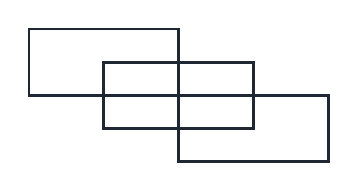
\begin{tikzpicture}[x=0.95cm,y=0.42cm]
\draw[Ink,line width=1pt] (0,2) rectangle (2,4);
\draw[Ink,line width=1pt] (1,1) rectangle (3,3);
\draw[Ink,line width=1pt] (2,0) rectangle (4,2);
\end{tikzpicture}
\end{minipage}
\end{probbox}
\probsol{
\textbf{Understanding the problem.} Call the three identical rectangles \textbf{I} (top left), \textbf{II} (middle) and \textbf{III} (bottom right). Where their sides cross, more small rectangles appear. We must count \emph{all} rectangles whose four sides are all drawn in the figure.
\step{1}{Look carefully at the figure}
Label the points as below. Notice: the bottom side of rectangle I and the top side of rectangle III lie on \emph{the same straight line} and join at the point $O$ -- the centre of rectangle II. Likewise the right side of I and the left side of III join at $O$. So inside rectangle II there is a ``plus sign'' that divides II into $4$ equal small cells.
\begin{center}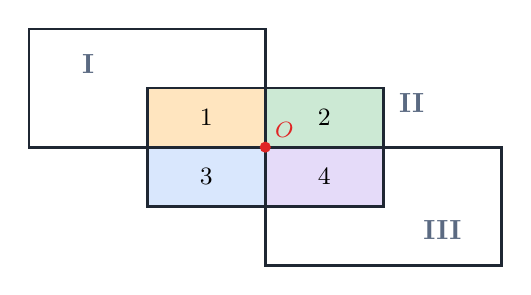
\begin{tikzpicture}[x=1.5cm,y=0.75cm,font=\sffamily\small]
\fill[tmOrange!25] (1,2) rectangle (2,3);\fill[tmGreen!25] (2,2) rectangle (3,3);
\fill[tmBlue!20] (1,1) rectangle (2,2);\fill[tmPurple!20] (2,1) rectangle (3,2);
\draw[Ink,line width=1pt] (0,2) rectangle (2,4);
\draw[Ink,line width=1pt] (1,1) rectangle (3,3);
\draw[Ink,line width=1pt] (2,0) rectangle (4,2);
\node at (1.5,2.5){$1$};\node at (2.5,2.5){$2$};\node at (1.5,1.5){$3$};\node at (2.5,1.5){$4$};
\fill[AnsRed] (2,2) circle (2pt);\node[above right,font=\footnotesize\bfseries,text=AnsRed] at (2,2){$O$};
\node[font=\bfseries,text=Slate] at (0.5,3.4){I};\node[font=\bfseries,text=Slate] at (3.5,0.6){III};
\node[font=\bfseries,text=Slate,anchor=west] at (3.05,2.75){II};
\end{tikzpicture}\end{center}
\step{2}{Count type by type}
\begin{itemize}[leftmargin=1.2em,itemsep=1pt,topsep=1pt]
\item \textbf{The three original large rectangles:} I, II, III -- $3$ rectangles.
\item \textbf{The four small cells} inside rectangle II (cells $1$, $2$, $3$, $4$) -- $4$ rectangles. Each cell has all four sides: for example cell $1$ has its top and left sides on rectangle II, and its bottom and right sides on rectangle I.
\item \textbf{Halves of rectangle II} (two neighbouring cells joined): cells $1+2$ (top half), $3+4$ (bottom half), $1+3$ (left half), $2+4$ (right half) -- $4$ rectangles.
\end{itemize}
\step{3}{Check that there are no others}
\begin{itemize}[leftmargin=1.2em,itemsep=1pt,topsep=1pt]
\item The part of rectangle I \emph{outside} rectangle II is L-shaped, and no segment passes through it. A rectangle containing part of this L-shaped region must use the left side and the top side of rectangle I as its sides; these two sides are exactly as long as the sides of rectangle I, so that rectangle is rectangle I itself. Likewise, a rectangle containing part of III outside II can only be rectangle III.
\item Every other rectangle must lie entirely inside rectangle II. Rectangle II with its inner ``plus sign'' is a $2\times2$ grid of cells, and in Step 2 we have listed them all: $4$ cells, $4$ halves and rectangle II itself.
\end{itemize}
\begin{warnbox}Do not count the large rectangle surrounding all three shapes (from the top-left corner of I to the bottom-right corner of III): \emph{none} of its sides is fully drawn. And do not miss the small cells created by the ``plus sign'' in the centre.\end{warnbox}
\step{4}{Add up}
$3+4+4=11$ rectangles.
\verify{Another count -- inside rectangle II alone (a complete $2\times2$ grid): by Example 7 there are $9$ rectangles ($4$ cells, $4$ halves and II itself). Adding rectangles I and III: $9+2=11$ \checkmark.}
The answer is \textbf{(A)}.
\ans{(A) $11$}
}

% ---------------- part b ----------------
% ================= Topic 3 (EN) -- part b: problems 16--30 =================
\providecommand{\cpTooth}[3]{% #1 rows, #2 columns, #3 unit (cm): grid of toothpicks
  \foreach \j in {0,...,#1}{\foreach \i in {1,...,#2}{
    \draw[tmOrange!85!black,line width=1.6pt,line cap=round]
      ({(\i-1)*#3+0.05},{\j*#3})--({\i*#3-0.05},{\j*#3});}}
  \foreach \j in {1,...,#1}{\foreach \i in {0,...,#2}{
    \draw[tmOrange!85!black,line width=1.6pt,line cap=round]
      ({\i*#3},{(\j-1)*#3+0.05})--({\i*#3},{\j*#3-0.05});}}}

\begin{probbox}{16}{\relax}
On the dot grid shown, Lan stands at dot $A$. She tosses a fair coin to decide how to move: if the coin shows
\emph{heads} she moves \emph{up} one dot; if it shows \emph{tails} she moves \emph{right} one dot. After exactly four
tosses, Lan will stop at one of the five dots $P$, $Q$, $R$, $S$, $T$. What is the probability that Lan stops at dot $R$?
\begin{figC}\begin{scope}[scale=0.8]
  \foreach \y in {0,...,4}{\pgfmathtruncatemacro\m{4-\y}
    \foreach \x in {0,...,\m}{\fill[Navy] (\x,\y) circle (2.6pt);}}
  \node[below left] at (0,0) {$A$};
  \node[above right] at (0,4) {$P$};\node[above right] at (1,3) {$Q$};
  \node[above right] at (2,2) {$R$};\node[above right] at (3,1) {$S$};
  \node[above right] at (4,0) {$T$};
  \fill[tmOrange] (0,0) circle (3.4pt);
\end{scope}\end{figC}
\choices{$\dfrac12$}{$\dfrac38$}{$\dfrac9{16}$}{$\dfrac7{16}$}{$\dfrac5{16}$}
\end{probbox}
\probsol{
\textbf{Understanding the problem.} At each toss Lan moves \emph{up} ($\uparrow$, for heads) or \emph{right}
($\rightarrow$, for tails). After $4$ tosses she has made exactly $4$ moves. We need the probability that after these
$4$ moves she is at $R$.

\step{1}{Count all possible outcomes}
Each toss has $2$ outcomes (heads or tails), so four tosses in a row give
$2\times2\times2\times2=16$ sequences, for example $\uparrow\rightarrow\rightarrow\uparrow$.
Since the coin is fair, these $16$ sequences are \emph{equally likely}.
\begin{recallbox}\emph{Multiplication principle:} if the first task can be done in $a$ ways, the second in $b$ ways, \dots{} then
doing them one after another can be done in $a\times b\times\cdots$ ways. The \emph{probability} of an event (when the outcomes
are equally likely) $=\dfrac{\text{number of favourable outcomes}}{\text{number of possible outcomes}}$.\end{recallbox}

\step{2}{The final dot depends only on the number of up-moves}
If $k$ of the $4$ moves are up, then $4-k$ moves are to the right. The order of the moves does not change the final dot.
Starting from $A$: $4$ ups $\to P$; $3$ ups $\to Q$; $2$ ups $\to R$; $1$ up $\to S$; $0$ ups $\to T$.
So Lan stops at $R$ exactly when she makes \textbf{exactly $2$ moves up and $2$ moves right}.

\step{3}{List the favourable sequences}
We choose which two of the four turns (turn 1, 2, 3, 4) are $\uparrow$:
\[\uparrow\uparrow\rightarrow\rightarrow,\quad \uparrow\rightarrow\uparrow\rightarrow,\quad
\uparrow\rightarrow\rightarrow\uparrow,\quad \rightarrow\uparrow\uparrow\rightarrow,\quad
\rightarrow\uparrow\rightarrow\uparrow,\quad \rightarrow\rightarrow\uparrow\uparrow.\]
There are $6$ sequences (choosing $2$ turns out of $4$: $\dfrac{4\times3}{2}=6$ ways).

\step{4}{Compute the probability}
\[P(\text{stop at } R)=\frac{6}{16}=\frac38.\]

\step{5}{A picture: write the number of paths at each dot}
At each dot write the number of move sequences leading from $A$ to that dot. A dot can only be reached from the dot just to its
left or the dot just below it, so the number at each dot $=$ the sum of the numbers to its left and below (just like Pascal's triangle):
\begin{figC}\begin{scope}[scale=0.75]
  \foreach \x/\y/\n in {0/0/1,1/0/1,2/0/1,3/0/1,4/0/1,0/1/1,1/1/2,2/1/3,3/1/4,0/2/1,1/2/3,2/2/6,
     0/3/1,1/3/4,0/4/1}{
    \fill[tmBlue!12] (\x,\y) circle (9pt);
    \node[font=\small\bfseries,text=Navy] at (\x,\y) {\n};}
  \draw[AnsRed,thick] (2,2) circle (10pt);
  \node[right=10pt,text=AnsRed,font=\small] at (2,2) {$R$};
  \node[right=10pt,font=\small] at (4,0) {$T$};\node[right=10pt,font=\small] at (3,1) {$S$};
  \node[right=10pt,font=\small] at (1,3) {$Q$};\node[right=10pt,font=\small] at (0,4) {$P$};
\end{scope}\end{figC}
Along the last diagonal: $1+4+6+4+1=16$ (exactly the total number of sequences), and the number at $R$ is $6$.
\begin{warnbox}The five dots $P,Q,R,S,T$ are \emph{not} equally likely! Do not answer ``one of $5$ dots, so the probability is
$\frac15$''. The middle dot ($R$) can be reached in the most ways; each of the two end dots ($P$ and $T$) can be reached in only one way.\end{warnbox}
\verify{The probabilities of stopping at $P,Q,R,S,T$ are $\frac1{16},\frac4{16},\frac6{16},\frac4{16},\frac1{16}$;
they add up to $\frac{16}{16}=1$, as they should.}
The value $\frac38=\frac6{16}$ is option \textbf{(B)}.
\ans{(B) $\dfrac38$}
}

\begin{probbox}{17}{\relax}
Identical toothpicks are used to build rectangular grids of squares, as shown below. For example, the $1\times10$ grid
($1$ row of $10$ squares) uses $31$ toothpicks in total. How many toothpicks are needed for a $43\times10$ grid
($43$ rows, each with $10$ squares)?
\begin{figC}
  \begin{scope}[shift={(0,2.4)}]\cpTooth{1}{10}{0.42}\node[right] at (4.4,0.21) {$1\times10$};\end{scope}
  \begin{scope}[shift={(0,1.05)}]\cpTooth{2}{10}{0.42}\node[right] at (4.4,0.42) {$2\times10$};\end{scope}
  \begin{scope}[shift={(0,-0.6)}]\cpTooth{3}{10}{0.42}\node[right] at (4.4,0.63) {$3\times10$};\end{scope}
\end{figC}
\choices{$913$}{$860$}{$871$}{$903$}{$946$}
\end{probbox}
\probsol{
\textbf{Understanding the problem.} The $43\times10$ grid has $43$ rows of squares, $10$ squares in each row. The toothpicks lie in
two directions: \emph{horizontal} and \emph{vertical}. We count each kind separately and add (addition principle).

\step{1}{Check the method on the $1\times10$ grid}
\emph{Horizontal toothpicks:} the grid has $2$ horizontal lines (top edge and bottom edge), each made of $10$ toothpicks:
$2\times10=20$ toothpicks.
\emph{Vertical toothpicks:} there are $11$ vertical lines ($10$ squares need $11$ walls), each made of $1$ toothpick:
$11\times1=11$ toothpicks. Total: $20+11=31$, exactly as stated.
\begin{recallbox}A row of $10$ squares needs $10+1=11$ vertical walls (like the fence-post problem: $10$ gaps need $11$ posts).
In the same way, $43$ rows of squares have $43+1=44$ horizontal lines.\end{recallbox}

\step{2}{Count the horizontal toothpicks of the $43\times10$ grid}
There are $43+1=44$ horizontal lines, each $10$ toothpicks long: $44\times10=440$ toothpicks.

\step{3}{Count the vertical toothpicks of the $43\times10$ grid}
There are $10+1=11$ vertical lines, each $43$ toothpicks long (one toothpick per row): $11\times43=473$ toothpicks.

\step{4}{Add}
$440+473=913$ toothpicks.

\step{5}{Second method: add one row at a time}
The $1\times10$ grid has $31$ toothpicks. Each time a new row is placed on top, we need $10$ more horizontal toothpicks
(the top edge of the new row) and $11$ vertical ones, that is $21$ toothpicks (the bottom edge is already there). Going from
$1$ row to $43$ rows means adding $42$ rows:
\[31+42\times21=31+882=913.\]
\begin{warnbox}Do not compute $43\times31=1333$: when rows are stacked, two neighbouring rows \emph{share} a line of $10$ horizontal
toothpicks, so multiplying like that counts those toothpicks twice.\end{warnbox}
\verify{By the formula $(\text{rows}+1)\times10+11\times\text{rows}$: the $2\times10$ grid needs
$3\times10+11\times2=52$ toothpicks and the $3\times10$ grid needs $4\times10+11\times3=73$; counting directly in the picture also gives
$52$ and $73$. Both methods give the same result, $913$.}
So the answer is \textbf{(A)}.
\ans{(A) $913$ toothpicks}
}

\begin{probbox}{18}{\relax}
In the cafeteria at Minh's school, the meats are beef and chicken, and the fruits are apple, pear and banana. Minh is given a
random lunch consisting of one meat and one fruit. The probability that Minh's lunch includes a banana is
\choices{$\dfrac13$}{$\dfrac23$}{$\dfrac12$}{$\dfrac15$}{$\dfrac35$}
\end{probbox}
\probsol{
\textbf{Understanding the problem.} A lunch $=$ (one meat, one fruit). The lunch is chosen at random, so all possible lunches are
equally likely. We need the probability that the lunch includes a banana.

\step{1}{List all possible lunches}
By the multiplication principle there are $2\times3=6$ lunches. We make a table (rows: meat, columns: fruit):
\begin{center}\begin{tabular}{|c|c|c|c|}\hline
 & Apple & Pear & \cellcolor{tmOrange!20}Banana\\\hline
Beef & Beef--Apple & Beef--Pear & \cellcolor{tmOrange!20}Beef--Banana\\\hline
Chicken & Chicken--Apple & Chicken--Pear & \cellcolor{tmOrange!20}Chicken--Banana\\\hline
\end{tabular}\end{center}

\step{2}{Count the lunches with a banana}
The ``Banana'' column has $2$ lunches: Beef--Banana and Chicken--Banana.

\step{3}{Compute the probability}
\[P(\text{banana})=\frac{2}{6}=\frac13.\]
\begin{recallbox}To simplify a fraction, divide the numerator and the denominator by their greatest common divisor:
$\dfrac26=\dfrac{2\div2}{6\div2}=\dfrac13$.\end{recallbox}
\begin{tipbox}The meat has no effect on the fruit. A quicker way to think: the fruit is one of $3$ equally likely kinds, and banana is
$1$ of the $3$ kinds, so the probability is $\frac13$.\end{tipbox}
\begin{warnbox}Do not add ``$2$ meats $+\,3$ fruits $=5$'' and answer $\frac15$: the number of lunches is $2\times3=6$, not $2+3=5$.\end{warnbox}
\verify{The probabilities of getting an apple, a pear and a banana are all $\frac13$; they add up to $\frac13+\frac13+\frac13=1$.}
So the answer is \textbf{(A)}.
\ans{(A) $\dfrac13$}
}

\begin{probbox}{19}{\relax}
A special six-sided die is made, with one number written on each face (numbers may repeat). When this die is rolled, the probability
of getting a multiple of $3$ is $\frac12$, and the probability of getting an even number is $\frac13$.
The six numbers on the faces could be
\choicesII{$1,2,3,5,5,6$}{$1,2,3,3,5,6$}{$1,2,3,4,6,6$}{$1,2,3,3,4,6$}{$2,3,3,3,5,6$}
\end{probbox}
\probsol{
\textbf{Understanding the problem.} The die has $6$ equally likely faces. From the two given probabilities we work out the
\emph{number of faces} showing a multiple of $3$ and the number of faces showing an even number, then check each option.

\step{1}{Turn probabilities into numbers of faces}
\begin{recallbox}With $6$ equally likely faces: $P=\dfrac{\text{number of favourable faces}}{6}$, so
the number of favourable faces $=P\times6$.\end{recallbox}
Faces with a multiple of $3$: $\frac12\times6=3$ faces.\quad Even faces: $\frac13\times6=2$ faces.

So we need: \textbf{exactly $3$ faces that are multiples of $3$} and \textbf{exactly $2$ even faces}.

\step{2}{Check each option}
Among the numbers $1$ to $6$: the multiples of $3$ are $3$ and $6$; the even numbers are $2$, $4$, $6$.
Note that $6$ is both even and a multiple of $3$, so it must be counted in \emph{both} columns.
\begin{center}\begin{tabular}{|c|c|c|c|c|}\hline
Option & Faces & Multiples of $3$ & Even faces & OK?\\\hline
(A) & $1,2,3,5,5,6$ & $3,6$ \;($2$ faces) & $2,6$ \;($2$ faces) & No\\\hline
\rowcolor{tmGreen!12}(B) & $1,2,3,3,5,6$ & $3,3,6$ \;($3$ faces) & $2,6$ \;($2$ faces) & Yes\\\hline
(C) & $1,2,3,4,6,6$ & $3,6,6$ \;($3$ faces) & $2,4,6,6$ \;($4$ faces) & No\\\hline
(D) & $1,2,3,3,4,6$ & $3,3,6$ \;($3$ faces) & $2,4,6$ \;($3$ faces) & No\\\hline
(E) & $2,3,3,3,5,6$ & $3,3,3,6$ \;($4$ faces) & $2,6$ \;($2$ faces) & No\\\hline
\end{tabular}\end{center}
\begin{warnbox}If you forget that $6$ is even, you will count only $2$ even faces for (D) and wrongly choose (D).
A number can belong to several groups at once!\end{warnbox}
\verify{For (B): $P(\text{multiple of }3)=\frac36=\frac12$ and $P(\text{even})=\frac26=\frac13$; both conditions hold.}
Only option \textbf{(B)} works.
\ans{(B) $1,2,3,3,5,6$}
}

\begin{probbox}{20}{\stars{1}}
Three bus routes run along the roads shown in the figure, all passing through stop $X$ (segments with the same number of small marks
are equal: $PX=XS$, $QX=XT$, $RX=XU$).
\begin{itemize}[leftmargin=1.2em,itemsep=1pt,topsep=2pt]
\item Bus $A$ runs the route $P\to X\to S\to X\to P$; each round trip takes $12$ minutes.
\item Bus $B$ runs the route $Q\to X\to T\to X\to Q$; each round trip takes $20$ minutes.
\item Bus $C$ runs the route $R\to X\to U\to X\to R$; each round trip takes $28$ minutes.
\end{itemize}
At 1:00 p.m., buses $A$, $B$, $C$ leave $P$, $Q$, $R$ respectively. Each bus travels at a constant speed, turns around instantly
at both ends of its route and runs without stopping until 11:00 p.m. Between 5:00 p.m. and 10:00 p.m., at how many moments are two
or more buses at stop $X$ at the same time?
\begin{figC}\begin{scope}[scale=0.9]
  \draw[Ink,thick] (0,1.6)--(0,-1.6);\draw[Ink,thick] (-1.9,0)--(1.9,0);\draw[Ink,thick] (-2,-1.35)--(2,1.35);
  \foreach \p in {(0,1.6),(0,-1.6),(-1.9,0),(1.9,0),(-2,-1.35),(2,1.35),(0,0)}{\fill[Navy] \p circle (2pt);}
  \node[above] at (0,1.6) {$P$};\node[below] at (0,-1.6) {$S$};\node[left] at (-1.9,0) {$Q$};
  \node[right] at (1.9,0) {$T$};\node[below left] at (-2,-1.35) {$R$};\node[above right] at (2,1.35) {$U$};
  \node[below right] at (0.05,-0.02) {$X$};
  \draw[tmBlue,thick] (-0.12,0.8)--(0.12,0.8);\draw[tmBlue,thick] (-0.12,-0.8)--(0.12,-0.8);
  \foreach \s in {-1,1}{\draw[tmOrange,thick] (\s*0.95-0.04,-0.12)--(\s*0.95-0.04,0.12);
                        \draw[tmOrange,thick] (\s*0.95+0.04,-0.12)--(\s*0.95+0.04,0.12);}
  \foreach \s in {-1,1}{\foreach \d in {-0.09,0,0.09}{
     \draw[tmGreen!80!black,thick] ($(\s*1,\s*0.675)+(\d*0.829,\d*0.559)+(0.067,-0.1)$)--++(-0.134,0.2);}}
\end{scope}\end{figC}
\choices{$18$}{$19$}{$20$}{$21$}{$22$}
\end{probbox}
\probsol{
\textbf{Understanding the problem.} We measure time as \emph{the number of minutes after 1:00 p.m.} and call this number $t$.
We need the values of $t$ at which at least two buses are at $X$, with $t$ between 5:00 p.m. and 10:00 p.m.

\step{1}{Convert the time window into minutes}
5:00 p.m. is $4$ hours after 1:00 p.m.: $t=4\times60=240$. \quad 10:00 p.m. is $9$ hours after 1:00 p.m.: $t=9\times60=540$.
So we look at $240\le t\le540$.

\step{2}{When is bus $A$ at $X$?}
One round trip of bus $A$ consists of $4$ equal legs: $P\to X$, $X\to S$, $S\to X$, $X\to P$ (because $PX=XS$).
The bus moves at constant speed, so each leg takes $12\div4=3$ minutes. Bus $A$ reaches $X$ at the end of the first leg and at the end
of the third leg of every round trip, that is at
\[t=3,\ 9,\ 15,\ 21,\ 27,\ \dots\]
These are exactly the \textbf{odd multiples of $3$} ($3\times1$, $3\times3$, $3\times5$, \dots). At the end of the second and fourth legs
the bus is at $S$ or $P$, not at $X$.

\step{3}{The same for buses $B$ and $C$}
Bus $B$: each leg takes $20\div4=5$ minutes, so it is at $X$ when $t=5,15,25,35,\dots$ -- the \textbf{odd multiples of $5$}.\\
Bus $C$: each leg takes $28\div4=7$ minutes, so it is at $X$ when $t=7,21,35,49,\dots$ -- the \textbf{odd multiples of $7$}.

\step{4}{When do two buses meet at $X$?}
\begin{recallbox}A number divisible by both $3$ and $5$ is divisible by $\text{lcm}(3,5)=15$. Similarly:
divisible by both $3$ and $7$ $\Leftrightarrow$ divisible by $21$; divisible by both $5$ and $7$ $\Leftrightarrow$
divisible by $35$.\end{recallbox}
Buses $A$ and $B$ are both at $X$ when $t$ is an odd multiple of $3$ and also an odd multiple of $5$, that is when $t$ is an
\textbf{odd number divisible by $15$} (an odd multiple of $15$). Similarly: $A$ and $C$ meet when $t$ is an odd multiple of $21$;
$B$ and $C$ meet when $t$ is an odd multiple of $35$.
\begin{proofbox}An odd multiple of $15$ is an odd number divisible by $15$, so it is an odd number divisible by $3$ (an odd multiple of $3$)
and an odd number divisible by $5$ (an odd multiple of $5$). Conversely, a number that is an odd multiple of $3$ and an odd multiple of $5$ is
odd and divisible by $15$.\end{proofbox}

\step{5}{List them for $240\le t\le540$}
\begin{center}\begin{tabular}{|l|l|c|}\hline
Two buses & Values of $t$ (odd multiples) & Count\\\hline
$A$ and $B$ ($15$) & $255, 285, 315, 345, 375, 405, 435, 465, 495, 525$ & $10$\\\hline
$A$ and $C$ ($21$) & $273, 315, 357, 399, 441, 483, 525$ & $7$\\\hline
$B$ and $C$ ($35$) & $245, 315, 385, 455, 525$ & $5$\\\hline
\end{tabular}\end{center}
(For example, in the first row: $15\times17=255$ is the first odd multiple greater than $240$; after that we keep adding $30$, because
two consecutive odd multiples of $15$ are $2\times15=30$ apart.)

\step{6}{Remove the moments counted more than once}
Adding the three rows gives $10+7+5=22$, but the moments $315$ and $525$ appear in \emph{all three rows}
(they are odd multiples of $3\times5\times7=105$: at those moments all three buses are at $X$). Each of these moments is counted $3$ times
but should be counted only once, so we subtract $2+2=4$:
\[22-4=18 \text{ moments.}\]
\begin{warnbox}The question asks for the number of \emph{moments}, not the number of ``pairs of buses meeting''. When all three buses are at
$X$ together, that is just \emph{one} moment. Adding $10+7+5=22$ and choosing (E) is wrong.\end{warnbox}
\verify{In clock times: 5:05, 5:15, 5:33, 5:45, 6:15, 6:45, 6:57, 7:15, 7:25, 7:39, 7:45, 8:15, 8:21, 8:35, 8:45, 9:03, 9:15, 9:45 p.m.
-- exactly $18$ moments, all between 5:00 p.m. and 10:00 p.m.}
So the answer is \textbf{(A)}.
\ans{(A) $18$}
}

\begin{probbox}{21}{\relax}
Each face of a cube is painted with exactly one colour. What is the smallest number of colours needed to paint the cube so that any
two faces sharing an edge have different colours?
\choices{$2$}{$3$}{$4$}{$5$}{$6$}
\end{probbox}
\probsol{
\textbf{Understanding the problem.} Two faces ``sharing an edge'' are adjacent faces. Two opposite faces (such as the top and the
bottom) have no common edge, so they may have the same colour. We must (1) show a colouring that uses few colours, and
(2) prove that fewer colours are impossible.

\step{1}{Two colours are not enough}
\begin{proofbox}Look at any corner of the cube, for example the top--front--right corner. Three faces meet there: the top, the front and the
right face. Any two of these three faces share an edge, so the three faces must have three different colours. Hence at least $3$ colours
are needed.\end{proofbox}

\step{2}{Three colours are enough}
Paint \emph{each pair of opposite faces the same colour}: top and bottom blue, front and back orange, left and right green.
Each face is adjacent to $4$ faces, which are exactly the four faces \emph{not} opposite to it, and these four faces carry the other two
colours. So no two adjacent faces have the same colour.
\begin{figC}
  \begin{scope}
   \fill[tmOrange!55,draw=Ink,thick] (0,0)--(1.6,0)--(1.6,1.6)--(0,1.6)--cycle;
   \fill[tmBlue!55,draw=Ink,thick] (0,1.6)--(1.6,1.6)--(2.4,2.3)--(0.8,2.3)--cycle;
   \fill[tmGreen!55,draw=Ink,thick] (1.6,0)--(2.4,0.7)--(2.4,2.3)--(1.6,1.6)--cycle;
   \node at (0.8,0.8) {front};\node at (1.2,1.95) {top};\node at (2,1.15) {right};
  \end{scope}
  \begin{scope}[shift={(4,0.1)},scale=0.5]
   \foreach \x/\y/\c in {1/2/tmBlue,0/1/tmGreen,1/1/tmOrange,2/1/tmGreen,3/1/tmOrange,1/0/tmBlue}{
     \fill[\c!55,draw=Ink,thick] (\x,\y) rectangle ++(1,1);}
   \node[font=\scriptsize] at (2,-0.45) {net of the cube};
  \end{scope}
\end{figC}

\step{3}{Conclusion}
At least $3$ colours are needed (step 1) and $3$ colours are enough (step 2), so the smallest number of colours is $3$.
\begin{warnbox}Finding one colouring with $3$ colours is \emph{not enough} to claim that $3$ is the smallest; you must explain why $2$ colours
fail (the three faces at a corner). On the other hand, thinking ``$6$ faces need $6$ colours'' forgets that opposite faces may share a
colour.\end{warnbox}
\verify{On the net, each square shares edges only with squares of other colours (when folded, two squares of the same colour become
opposite faces).}
So the answer is \textbf{(B)}.
\ans{(B) $3$ colours}
}

\begin{probbox}{22}{\relax}
How many different pairs $(m,n)$ can be formed from the integers $1,2,3,\dots,20$ such that $m<n$ and $m+n$ is even?
\choices{$55$}{$90$}{$140$}{$110$}{$50$}
\end{probbox}
\probsol{
\textbf{Understanding the problem.} We choose two different numbers out of $20$; because $m<n$, each pair of two numbers is counted
\emph{only once} (the smaller one is $m$, the larger one is $n$). Condition: the sum $m+n$ is even.

\step{1}{When is the sum of two numbers even?}
\begin{recallbox}even $+$ even $=$ even;\quad odd $+$ odd $=$ even;\quad even $+$ odd $=$ odd.\end{recallbox}
So $m+n$ is even exactly when $m$ and $n$ have \textbf{the same parity} (both even or both odd).

\step{2}{Split the $20$ numbers into two groups}
Even group: $2,4,6,\dots,20$ -- $10$ numbers.\quad Odd group: $1,3,5,\dots,19$ -- $10$ numbers.

\step{3}{Count the pairs in the even group}
The first number can be chosen in $10$ ways and the second (different from the first) in $9$ ways: $10\times9=90$ \emph{ordered} choices.
But each pair, for example $\{2,4\}$, is counted twice ($2$ then $4$, or $4$ then $2$), while the condition $m<n$ allows only the order
$(2,4)$. So the number of pairs is $\dfrac{10\times9}{2}=45$.
\begin{recallbox}The number of ways to choose $2$ objects (order does not matter) from $k$ objects is $\dfrac{k\times(k-1)}{2}$.\end{recallbox}

\step{4}{Count the pairs in the odd group and add}
In the same way the odd group gives $45$ pairs. A pair cannot be in both groups, so by the addition principle:
$45+45=90$ pairs.
\begin{warnbox}Forgetting to divide by $2$ gives $90+90=180$ (not an option); forgetting the odd group gives $45$. Always ask yourself:
``Did I count a pair twice? Did I miss a case?''\end{warnbox}
\verify{Count using the complement: the total number of pairs with $m<n$ is $\dfrac{20\times19}{2}=190$. The number of pairs with different
parity (one even, one odd) is $10\times10=100$. So the number of pairs with the same parity is $190-100=90$. It matches!}
So the answer is \textbf{(B)}.
\ans{(B) $90$ pairs}
}

\begin{probbox}{23}{\stars{1}}
Two different two-digit positive integers are called a \emph{reversal pair} if one is obtained from the other by swapping its two digits.
For example, $52$ and $25$ form a reversal pair. The number $2015$ has a special property: it is the product of three different prime
numbers, two of which form a reversal pair ($2015=5\times13\times31$). Including $2015$, how many positive integers less than $10\,000$
have this same property?
\choices{$18$}{$14$}{$20$}{$17$}{$19$}
\end{probbox}
\probsol{
\textbf{Understanding the problem.} We must count the numbers $N<10\,000$ of the form $N=p\times q\times r$, where $p,q,r$ are three
different primes and two of them (call them $p$ and $q$) form a two-digit reversal pair. Plan: find all reversal pairs made of two primes,
then for each pair find the suitable third primes.

\step{1}{Find the reversal pairs in which both numbers are prime}
\begin{recallbox}A prime number is a natural number greater than $1$ whose only divisors are $1$ and itself. The two-digit primes are:
$11, 13, 17, 19, 23, 29, 31, 37, 41, 43, 47, 53, 59, 61, 67, 71, 73, 79, 83, 89, 97$.\end{recallbox}
\begin{tipbox}The units digit of the reversal of $p$ is the tens digit of $p$. A two-digit prime must end in $1,3,7$ or $9$, so we only need
to look at primes starting with $1,3,7,9$: $11,13,17,19,31,37,71,73,79,97$.\end{tipbox}
Check the reversal of each one:
\begin{center}\begin{tabular}{|c|c|c|c|c|c|c|c|c|c|c|}\hline
$p$ & $11$ & $13$ & $17$ & $19$ & $31$ & $37$ & $71$ & $73$ & $79$ & $97$\\\hline
reversal & $11$ & $31$ & $71$ & $91$ & $13$ & $73$ & $17$ & $37$ & $97$ & $79$\\\hline
prime? & same & yes & yes & no & yes & yes & yes & yes & yes & yes\\\hline
\end{tabular}\end{center}
($91=7\times13$ is not prime; $11$ reversed is still $11$, so it does not give two \emph{different} numbers.)
So there are exactly $4$ pairs: $\{13,31\}$, $\{17,71\}$, $\{37,73\}$, $\{79,97\}$.

\step{2}{Compute the product of each pair}
$13\times31=403$;\quad $17\times71=1207$;\quad $37\times73=2701$;\quad $79\times97=7663$.

\step{3}{Find the third prime $r$ for each pair}
We need $r$ prime, different from the two numbers of the pair, and the product $<10\,000$.
\begin{itemize}[leftmargin=1.2em,itemsep=1pt,topsep=2pt]
\item Pair $\{13,31\}$: we need $403\times r<10\,000$. Since $403\times24=9672$ and $403\times25=10\,075$, we need $r\le23$.
The primes $\le23$ are $2,3,5,7,11,13,17,19,23$; remove $13$ (already in the pair): $8$ primes remain, giving
$806;\ 1209;\ 2015;\ 2821;\ 4433;\ 6851;\ 7657;\ 9269$.
\item Pair $\{17,71\}$: we need $1207\times r<10\,000$; since $1207\times8=9656$ and $1207\times9=10\,863$, $r\le8$:
$r\in\{2,3,5,7\}$, giving $2414;\ 3621;\ 6035;\ 8449$ ($4$ numbers).
\item Pair $\{37,73\}$: $2701\times3=8103<10\,000$ and $2701\times4>10\,000$, so $r\in\{2,3\}$: $5402;\ 8103$ ($2$ numbers).
\item Pair $\{79,97\}$: even $7663\times2=15\,326>10\,000$, so there are none.
\end{itemize}

\step{4}{Check that no number is counted twice, and add}
\begin{proofbox}Every number has only one prime factorisation. If a number appeared in two lists, then among its three prime factors there
would be two different reversal pairs; these two pairs would have to share a prime. But the table in step 1 shows that each prime belongs
to exactly one pair. So no number is counted twice.\end{proofbox}
In total: $8+4+2+0=14$ numbers.
\begin{warnbox}Two common mistakes: (1) forgetting that the third prime must be \emph{different} from the two primes of the pair, and so
also counting $403\times13=5239=13\times13\times31$ (wrong, since $13$ is repeated); (2) forgetting the prime $2$.\end{warnbox}
\verify{$2015=403\times5$ is in the list. Checking a few numbers: $9269=13\times31\times23$, $8449=17\times71\times7$,
$8103=37\times73\times3$; all are less than $10\,000$.}
So the answer is \textbf{(B)}.
\ans{(B) $14$}
}

\begin{probbox}{24}{\relax}
The figure is made of $8$ identical small parallelograms. Including these $8$ small parallelograms, how many parallelograms are there in
the figure altogether?
\begin{figC}
  \foreach \j in {0,1,2}{\draw[Ink,thick] (\j*0.55,\j*0.8)--(4.4+\j*0.55,\j*0.8);}
  \foreach \i in {0,...,4}{\draw[Ink,thick] (\i*1.1,0)--(\i*1.1+1.1,1.6);}
\end{figC}
\choices{$29$}{$30$}{$26$}{$27$}{$28$}
\end{probbox}
\probsol{
\textbf{Understanding the problem.} The figure has $2$ rows, each with $4$ small parallelograms. Every parallelogram in the figure is
formed from the segments already drawn: two of its sides lie on \emph{horizontal lines} and two lie on \emph{slanted lines}.

\step{1}{Count the lines in the figure}
There are $3$ horizontal lines (bottom, middle, top) and $5$ slanted lines (parallel to each other).
\begin{figC}
  \foreach \j/\l in {0/1,1/2,2/3}{\draw[tmBlue,thick] (\j*0.55,\j*0.8)--(4.4+\j*0.55,\j*0.8);
     \node[left,text=tmBlue,font=\scriptsize] at (\j*0.55,\j*0.8) {horiz.\ \l};}
  \foreach \i in {0,...,4}{\draw[tmOrange,thick] (\i*1.1,0)--(\i*1.1+1.1,1.6);
     \pgfmathtruncatemacro\k{\i+1}\node[below,text=tmOrange!80!black,font=\scriptsize] at (\i*1.1,0) {s\k};}
  \fill[tmGreen!30,opacity=0.7] (1.1,0)--(3.3,0)--(3.85,0.8)--(1.65,0.8)--cycle;
\end{figC}
For example, the green parallelogram is determined by horizontal lines $1$ and $2$ and slanted lines s$2$ and s$4$.

\step{2}{Each parallelogram corresponds to a choice of $2$ horizontal lines and $2$ slanted lines}
Choosing $2$ of the $3$ horizontal lines as bottom and top sides, and $2$ of the $5$ slanted lines as left and right sides, gives exactly
one parallelogram; conversely, every parallelogram in the figure comes from exactly one such choice.
\begin{recallbox}The number of ways to choose $2$ lines out of $k$ lines is $\dfrac{k\times(k-1)}{2}$.\end{recallbox}
Choosing $2$ horizontal lines: $\dfrac{3\times2}{2}=3$ ways. \quad Choosing $2$ slanted lines: $\dfrac{5\times4}{2}=10$ ways.

\step{3}{Apply the multiplication principle}
Number of parallelograms: $3\times10=30$.

\step{4}{Check by counting by size}
Call a parallelogram ``height $a$, width $b$'' if it is made of $a$ rows and $b$ columns of small ones:
\begin{center}\begin{tabular}{|c|c|c|c|c|c|}\hline
 & width $1$ & width $2$ & width $3$ & width $4$ & Total\\\hline
height $1$ ($2$ positions in rows) & $2\times4=8$ & $2\times3=6$ & $2\times2=4$ & $2\times1=2$ & $20$\\\hline
height $2$ ($1$ position in rows) & $4$ & $3$ & $2$ & $1$ & $10$\\\hline
\end{tabular}\end{center}
\begin{warnbox}Do not just count the $8$ small ones plus a few ``obvious'' big ones. Count systematically: by size (table above) or by
choosing lines.\end{warnbox}
\verify{The table gives $20+10=30$, the same as $3\times10$.}
So the answer is \textbf{(B)}.
\ans{(B) $30$ parallelograms}
}

\begin{probbox}{25}{\stars{1}}
A jar contains $2$ red marbles and $2$ blue marbles and no other marbles. Hoa randomly takes $2$ marbles out of the jar at the same time.
If the two marbles have the same colour, she throws one away and puts the other back into the jar. If they have different colours, she
throws away the red marble and puts the blue marble back into the jar. Hoa does this three times in total. The probability that the last
marble left in the jar is red is
\choices{$\dfrac12$}{$\dfrac14$}{$\dfrac23$}{$\dfrac13$}{$0$}
\end{probbox}
\probsol{
\textbf{Understanding the problem.} Each draw removes exactly $1$ marble from the jar. After $3$ draws, $1$ of the $4$ marbles is left.
We follow the \emph{state} of the jar, written (number of red, number of blue), starting from $(2\text{R},2\text{B})$.

\step{1}{First draw, from $(2\text{R},2\text{B})$}
Call the marbles R$_1$, R$_2$, B$_1$, B$_2$. There are $6$ equally likely ways to take $2$ marbles:
R$_1$R$_2$;\ B$_1$B$_2$;\ R$_1$B$_1$;\ R$_1$B$_2$;\ R$_2$B$_1$;\ R$_2$B$_2$.
\begin{itemize}[leftmargin=1.2em,itemsep=1pt,topsep=2pt]
\item Two reds ($1$ way): throw away $1$ red $\to(1\text{R},2\text{B})$.
\item Two blues ($1$ way): throw away $1$ blue $\to(2\text{R},1\text{B})$.
\item Different colours ($4$ ways): throw away the red $\to(1\text{R},2\text{B})$.
\end{itemize}
So after draw $1$: state $(1\text{R},2\text{B})$ with probability $\frac56$, state $(2\text{R},1\text{B})$ with probability $\frac16$.

\step{2}{Second draw}
From $(1\text{R},2\text{B})$: $3$ ways to draw; $2$ ways give different colours $\to(0\text{R},2\text{B})$; $1$ way gives two blues $\to(1\text{R},1\text{B})$.\\
From $(2\text{R},1\text{B})$: $3$ ways to draw; $1$ way gives two reds $\to(1\text{R},1\text{B})$; $2$ ways give different colours $\to(1\text{R},1\text{B})$.
So from $(2\text{R},1\text{B})$ we certainly go to $(1\text{R},1\text{B})$.

\step{3}{Third draw}
From $(0\text{R},2\text{B})$: two blues are drawn, one is thrown away $\to(0\text{R},1\text{B})$.\\
From $(1\text{R},1\text{B})$: different colours are drawn, the red is thrown away $\to(0\text{R},1\text{B})$.
\begin{figC}
  \tikzset{st/.style={draw=tmBlue,fill=tmBlue!8,rounded corners=3pt,inner sep=3pt,font=\footnotesize}}
  \node[st] (a) at (0,0) {$2$R, $2$B};
  \node[st] (b) at (2.8,0.9) {$1$R, $2$B};\node[st] (c) at (2.8,-0.9) {$2$R, $1$B};
  \node[st] (d) at (5.6,0.9) {$0$R, $2$B};\node[st] (e) at (5.6,-0.9) {$1$R, $1$B};
  \node[st,draw=AnsRed,fill=AnsRed!8] (f) at (8.2,0) {$0$R, $1$B};
  \draw[->,thick,Slate] (a)--node[above,font=\scriptsize]{$\frac56$}(b);
  \draw[->,thick,Slate] (a)--node[below,font=\scriptsize]{$\frac16$}(c);
  \draw[->,thick,Slate] (b)--node[above,font=\scriptsize]{$\frac23$}(d);
  \draw[->,thick,Slate] (b)--node[above right,font=\scriptsize,pos=0.3]{$\frac13$}(e);
  \draw[->,thick,Slate] (c)--node[below,font=\scriptsize]{$1$}(e);
  \draw[->,thick,Slate] (d)--node[above,font=\scriptsize]{$1$}(f);
  \draw[->,thick,Slate] (e)--node[below,font=\scriptsize]{$1$}(f);
  \node[font=\scriptsize,text=Slate] at (1.4,-1.7) {draw 1};\node[font=\scriptsize,text=Slate] at (4.2,-1.7) {draw 2};
  \node[font=\scriptsize,text=Slate] at (6.9,-1.7) {draw 3};
\end{figC}
Every branch ends at $(0\text{R},1\text{B})$: the last marble is \textbf{always} blue.

\step{4}{Why -- without drawing the tree}
\begin{proofbox}Look at the number of blue marbles. Whenever at least one of the two marbles drawn is blue, Hoa always puts a blue marble back
into the jar (two blues: she puts one back; different colours: she puts the blue back). The number of blue marbles decreases only when two
blues are drawn, and then the one that was put back is still there. So the jar \emph{always contains at least one blue marble}. When only one
marble is left, it must be blue.\end{proofbox}
Therefore the event ``the last marble is red'' is an \emph{impossible event}, with probability $0$.
\begin{recallbox}An impossible event (one that never happens) has probability $0$; a certain event has probability $1$.\end{recallbox}
\begin{warnbox}Seeing ``$2$ red, $2$ blue'' and immediately guessing $\frac12$ is a trap: the throwing-away rule is \emph{not symmetric}
in the two colours (with different colours, the red one is always thrown away).\end{warnbox}
\verify{Total probability of reaching the final state $(0\text{R},1\text{B})$: $\frac56\cdot\frac23+\frac56\cdot\frac13+\frac16\cdot1=\frac{10}{18}+\frac{5}{18}+\frac{3}{18}=1$.}
So the answer is \textbf{(E)}.
\ans{(E) $0$}
}

\begin{probbox}{26}{\stars{1}}
On the $10\times10$ grid of squares shown, triangle $FGH$ is drawn. Point $P$ can be any of the $41$ points where grid lines cross
that lie \emph{inside} (not on the sides of) triangle $FGH$. For each position of $P$, exactly three triangles are formed: $FPG$, $GPH$,
$HPF$. Among all $41\times3=123$ of these triangles, how many have an area equal to exactly half the area of triangle $FGH$?
\begin{figC}\begin{scope}[scale=0.3]
  \draw[Line,thin] (0,0) grid (10,10);
  \draw[Ink,line width=1.3pt] (0,0)--(10,0)--(5,10)--cycle;
  \node[above,font=\scriptsize] at (5,10) {$F$};\node[below left,font=\scriptsize] at (0,0) {$G$};
  \node[below right,font=\scriptsize] at (10,0) {$H$};
\end{scope}\end{figC}
\choices{$5$}{$7$}{$3$}{$11$}{$9$}
\end{probbox}
\probsol{
\textbf{Understanding the problem.} Take the side of one small square as the unit and put $G$ at the bottom-left corner. Then $G$ and $H$
are the two bottom corners ($GH=10$) and $F$ is the midpoint of the top side. Each grid point is named by two numbers (squares to the
right, squares up); for example $G=(0,0)$, $H=(10,0)$, $F=(5,10)$.

\step{1}{Area of triangle $FGH$ and half of it}
\begin{recallbox}Area of a triangle $=\dfrac12\times\text{base}\times\text{corresponding height}$.\end{recallbox}
$\text{Area}(FGH)=\frac12\times10\times10=50$. Half of it is $25$.

\step{2}{Triangle $GPH$: the easiest}
Triangle $GPH$ has base $GH=10$, and its height is the distance from $P$ down to $GH$, that is the ``height'' $h$ of $P$ (the number of
squares above the bottom). $\text{Area}(GPH)=\frac12\times10\times h=5h$. We need $5h=25$, so $h=5$: $P$ lies on the $5$th horizontal grid
line. At height $5$ (half the height) the triangle is half as wide as its base, from $2.5$ to $7.5$. The grid points strictly \emph{inside}
on that segment are $(3,5),(4,5),(5,5),(6,5),(7,5)$: $\mathbf{5}$ points.

\step{3}{Triangle $FPG$: using a parallel line}
\begin{recallbox}Triangles with a common base whose third vertices lie on a line parallel to the base have the same height, so they have the
same area.\end{recallbox}
Let $M=(5,0)$ be the midpoint of $GH$. Triangle $FMG$ has base $GM=5$ and height $10$, so $\text{Area}(FMG)=\frac12\times5\times10=25$.
So every point $P$ on the line through $M$ parallel to $FG$ gives $\text{Area}(FPG)=25$.
\begin{proofbox}If $P$ is farther from $FG$ than that line, the height of triangle $FPG$ (on base $FG$) is larger, so the area is more than
$25$; if $P$ is closer to $FG$, the area is less than $25$. So $\text{Area}(FPG)=25$ \emph{only when} $P$ lies on that line.\end{proofbox}
Side $FG$ goes from $(0,0)$ to $(5,10)$: for every $1$ square to the right it goes up $2$ squares. The parallel line through $M=(5,0)$ does the
same: it passes through $(5,0)$, $(6,2)$, $(7,4)$ and then meets side $FH$ at $(7.5,\,5)$ (the midpoint of $FH$). The grid points
\emph{inside} the triangle are $(6,2)$ and $(7,4)$: $\mathbf{2}$ points. ($M$ lies on side $GH$, so it is excluded.)

\step{4}{Triangle $HPF$: by symmetry}
The figure is symmetric about the vertical line through $F$, so similarly there are $\mathbf{2}$ points: $(4,2)$ and $(3,4)$.
\begin{figC}\begin{scope}[scale=0.42]
  \draw[Line,thin] (0,0) grid (10,10);
  \draw[Ink,line width=1.2pt] (0,0)--(10,0)--(5,10)--cycle;
  \draw[tmBlue,line width=1.2pt] (2.5,5)--(7.5,5);
  \draw[tmOrange,line width=1.2pt] (5,0)--(7.5,5);\draw[tmGreen!80!black,line width=1.2pt] (5,0)--(2.5,5);
  \foreach \p in {(3,5),(4,5),(5,5),(6,5),(7,5)}{\fill[tmBlue] \p circle (5pt);}
  \foreach \p in {(6,2),(7,4)}{\fill[tmOrange] \p circle (5pt);}
  \foreach \p in {(4,2),(3,4)}{\fill[tmGreen!80!black] \p circle (5pt);}
  \node[above,font=\scriptsize] at (5,10) {$F$};\node[below left,font=\scriptsize] at (0,0) {$G$};
  \node[below right,font=\scriptsize] at (10,0) {$H$};\node[below,font=\scriptsize] at (5,0) {$M$};
  \node[right,font=\scriptsize,text=tmBlue,align=left] at (10.4,6) {blue: area $GPH=25$};
  \node[right,font=\scriptsize,text=tmOrange!80!black] at (10.4,4.6) {orange: area $FPG=25$};
  \node[right,font=\scriptsize,text=tmGreen!70!black] at (10.4,3.2) {green: area $HPF=25$};
\end{scope}\end{figC}

\step{5}{Add}
Number of triangles with area $25$: $5+2+2=9$. (One point $P$ cannot give two triangles of area $25$, because then the third triangle would
have area $50-25-25=0$, while $P$ lies strictly inside. So no triangle is missed or counted twice.)
\verify{For $P=(6,2)$: triangle $FPG$ fits in the rectangle from $(0,0)$ to $(6,10)$, of area $60$. Cut off three right triangles:
$\frac12\times6\times2=6$, $\frac12\times1\times8=4$ and $\frac12\times5\times10=25$. What remains is $60-6-4-25=25$. Correct!}
So the answer is \textbf{(E)}.
\ans{(E) $9$ triangles}
}

\begin{probbox}{27}{\relax}
A $10\times10$ square grid is made of $100$ points, as shown. Point $P$ is marked. One of the other $99$ points is chosen at random to be
$Q$. The probability that segment $PQ$ is horizontal or vertical is
\begin{figC}\begin{scope}[scale=0.38]
  \foreach \x in {0,...,9}{\foreach \y in {0,...,9}{\fill[Navy] (\x,\y) circle (3.2pt);}}
  \fill[white] (6,3) circle (6pt);\draw[tmOrange,line width=1.2pt] (6,3) circle (6pt);
  \node[above right,font=\scriptsize,text=tmOrange!80!black] at (6,3) {$P$};
\end{scope}\end{figC}
\choices{$\dfrac2{11}$}{$\dfrac15$}{$\dfrac1{10}$}{$\dfrac4{25}$}{$\dfrac5{33}$}
\end{probbox}
\probsol{
\textbf{Understanding the problem.} $Q$ is chosen at random among $99$ points (not counting $P$), all equally likely.
Segment $PQ$ is horizontal when $Q$ is in the same row as $P$, and vertical when $Q$ is in the same column as $P$.

\step{1}{Number of possible outcomes}
There are $100-1=99$ ways to choose $Q$.

\step{2}{Number of favourable outcomes}
The row containing $P$ has $10$ points; without $P$ there are $9$. The column containing $P$ has $10$ points; without $P$ there are $9$.
A point other than $P$ cannot be in both the same row and the same column as $P$ (the only such point is $P$ itself), so no point is
counted twice: $9+9=18$ points in total.
\begin{figC}\begin{scope}[scale=0.3]
  \foreach \x in {0,...,9}{\foreach \y in {0,...,9}{\fill[Slate!50] (\x,\y) circle (3pt);}}
  \foreach \x in {0,...,9}{\fill[tmBlue] (\x,3) circle (5pt);}
  \foreach \y in {0,...,9}{\fill[tmGreen!80!black] (6,\y) circle (5pt);}
  \fill[white] (6,3) circle (6pt);\draw[tmOrange,line width=1.2pt] (6,3) circle (6pt);
  \node[right,font=\scriptsize,text=tmBlue] at (10,3) {$9$ points in the same row};
  \node[above,font=\scriptsize,text=tmGreen!70!black] at (6,9.3) {$9$ points in the same column};
\end{scope}\end{figC}

\step{3}{Compute the probability}
\[P=\frac{18}{99}=\frac{18\div9}{99\div9}=\frac{2}{11}.\]
\begin{warnbox}The denominator is $99$, not $100$, because $Q$ must be different from $P$. Using $100$ gives $\frac{18}{100}$, which is not
an option. Also do not count $10+10=20$ points (that counts $P$ twice).\end{warnbox}
\begin{tipbox}The position of $P$ in the grid does not matter: every point has exactly $9$ points in its row and $9$ points in its column.\end{tipbox}
\verify{$\frac2{11}\times99=18$, exactly the number of favourable points.}
So the answer is \textbf{(A)}.
\ans{(A) $\dfrac2{11}$}
}

\begin{probbox}{28}{\stars{1}}
The sum of all the digits of the integers from $98$ to $101$ is
\[9+8+9+9+1+0+0+1+0+1=38.\]
What is the sum of all the digits of the integers from $1$ to $2008$?
\choices{$30\,054$}{$27\,018$}{$28\,036$}{$30\,036$}{$28\,054$}
\end{probbox}
\probsol{
\textbf{Understanding the problem.} Writing out $2008$ numbers and adding is far too long. We split them into three blocks: $1$ to $999$;
$1000$ to $1999$; $2000$ to $2008$, and find the digit sum of each block by counting \emph{how many times each digit appears}.

\step{1}{Block $1$ to $999$: write leading zeros to get three digits}
Write the numbers from $0$ to $999$ with three digits: $000, 001, 002, \dots, 998, 999$. Adding leading zeros and the number $000$
\emph{does not change} the digit sum. There are $1000$ numbers, that is $3000$ digits.
\begin{proofbox}In the units place the digits repeat in the cycle $0,1,2,\dots,9$; $1000$ numbers contain $100$ cycles, so each digit
$0$--$9$ appears exactly $100$ times. In the tens place each digit appears $10$ times in a row ($00$--$09$ have tens digit $0$, \dots)
and this repeats $10$ times: again $100$ times. In the hundreds place: $000$--$099$ have hundreds digit $0$ ($100$ times), \dots,
$900$--$999$ have hundreds digit $9$ ($100$ times). So in each place, each digit appears $100$ times.\end{proofbox}
Hence each digit $0,1,\dots,9$ appears $3\times100=300$ times. The digit sum is
\[300\times(0+1+2+\dots+9)=300\times45=13\,500.\]
\begin{recallbox}$0+1+2+\dots+9=\dfrac{9\times10}{2}=45$ (pair them up: $0+9=1+8=\dots=4+5=9$, and there are $5$ pairs).\end{recallbox}

\step{2}{Block $1000$ to $1999$}
Each number has the form $1\,abc$ where $abc$ runs from $000$ to $999$. The last three digits give $13\,500$ (as in step 1). The thousands
digit is $1$, appearing $1000$ times, which adds $1000$. Total: $13\,500+1000=14\,500$.

\step{3}{Block $2000$ to $2008$}
There are $9$ numbers. The thousands digit $2$ contributes $9\times2=18$; the two middle digits are $0$; the units digits are
$0,1,\dots,8$, contributing $0+1+\dots+8=36$. Total: $18+36=54$.

\step{4}{Add the three blocks}
\[13\,500+14\,500+54=28\,054.\]
\begin{warnbox}Do not forget the last small block $2000$--$2008$ (forgetting it gives $28\,000$), and do not forget the thousands digit $1$
in the second block (forgetting it gives $27\,054$).\end{warnbox}
\verify{Test the method on a small case, $1$ to $99$: each digit appears $2\times10=20$ times, sum $20\times45=900$. Directly: the units
place contributes $10\times45=450$ and the tens place contributes $10\times(1+2+\dots+9)=450$, total $900$. It matches.}
So the answer is \textbf{(E)}.
\ans{(E) $28\,054$}
}

\begin{probbox}{29}{\relax}
Two fair dice are rolled, one red and one blue (each has six faces numbered $1$ to $6$). The probability that the number on the red die
is greater than the number on the blue die is
\choices{$\dfrac{18}{36}$}{$\dfrac{25}{36}$}{$\dfrac{15}{36}$}{$\dfrac{12}{36}$}{$\dfrac{17}{36}$}
\end{probbox}
\probsol{
\textbf{Understanding the problem.} An outcome is a pair (number on the red die, number on the blue die). The dice have different
colours, so $(5,2)$ and $(2,5)$ are different outcomes.

\step{1}{Number of possible outcomes}
By the multiplication principle: $6\times6=36$ equally likely outcomes.

\step{2}{Make a table and mark the cells ``red $>$ blue''}
\begin{figC}\begin{scope}[scale=0.5]
  \foreach \r in {1,...,6}{\foreach \b in {1,...,6}{
    \pgfmathsetmacro\yy{6-\r}
    \ifnum\r>\b \fill[AnsRed!25] (\b-1,\yy) rectangle ++(1,1);
    \else\ifnum\r=\b \fill[Slate!20] (\b-1,\yy) rectangle ++(1,1);\fi\fi}}
  \draw[Ink] (0,0) grid (6,6);
  \foreach \i in {1,...,6}{\node[font=\scriptsize,text=tmBlue] at (\i-0.5,6.4) {\i};
     \node[font=\scriptsize,text=AnsRed] at (-0.4,6.5-\i) {\i};}
  \node[font=\scriptsize,text=tmBlue] at (3,7.1) {blue die};
  \node[font=\scriptsize,text=AnsRed,rotate=90] at (-1.2,3) {red die};
\end{scope}\end{figC}
Red cells: the red number is greater than the blue number; grey cells: the two numbers are equal. Count row by row (red number):
red $=1$: $0$ cells; red $=2$: $1$ cell; red $=3$: $2$ cells; red $=4$: $3$ cells; red $=5$: $4$ cells; red $=6$: $5$ cells.
Total: $0+1+2+3+4+5=15$ favourable outcomes.

\step{3}{Compute the probability}
$P(\text{red}>\text{blue})=\dfrac{15}{36}$.

\step{4}{A quick way: use symmetry}
There are $6$ outcomes where the two numbers are equal (the diagonal). The other $36-6=30$ outcomes split equally between ``red is
greater'' and ``blue is greater'' (swap the roles of the dice), so each kind has $30\div2=15$ outcomes.
\begin{warnbox}The answer $\frac{18}{36}=\frac12$ is a trap: it forgets the cases where the two numbers are equal. ``Red is greater'' and
``blue is greater'' are not the only possibilities.\end{warnbox}
\verify{$P(\text{red}>\text{blue})+P(\text{equal})+P(\text{blue}>\text{red})=\frac{15}{36}+\frac6{36}+\frac{15}{36}=1$.}
So the answer is \textbf{(C)}.
\ans{(C) $\dfrac{15}{36}$}
}

\begin{probbox}{30}{\relax}
Two fair dice are rolled, one red and one blue. The probability that the \emph{product} of the two numbers shown is even is
\choices{$\dfrac12$}{$\dfrac34$}{$\dfrac14$}{$\dfrac23$}{$\dfrac{11}{36}$}
\end{probbox}
\probsol{
\textbf{Understanding the problem.} As in problem 29, there are $6\times6=36$ equally likely outcomes. Counting the even products directly
is rather long, so we count the \emph{complement}: the outcomes with an odd product.

\step{1}{When is the product of two numbers odd?}
\begin{recallbox}odd $\times$ odd $=$ odd;\quad even $\times$ (any number) $=$ even. So the product of two numbers is odd exactly when
\emph{both} numbers are odd.\end{recallbox}

\step{2}{Count the outcomes with an odd product}
Odd numbers on each die: $1,3,5$ ($3$ numbers). Both dice odd: $3\times3=9$ outcomes.

\step{3}{Count the outcomes with an even product using the complement}
\begin{recallbox}\emph{Complement}: number of favourable outcomes $=$ number of possible outcomes $-$ number of unfavourable outcomes.
Likewise, $P(\text{event})=1-P(\text{event does not happen})$.\end{recallbox}
Number of outcomes with an even product: $36-9=27$.

\step{4}{Compute the probability}
\[P(\text{even product})=\frac{27}{36}=\frac{27\div9}{36\div9}=\frac34.\]
\begin{warnbox}Many students think ``even and odd are half and half'' and choose $\frac12$. But just \emph{one} even number makes the product
even, so an even product happens much more often.\end{warnbox}
\verify{Direct count: red die even ($3$ ways) with any blue number ($6$ ways): $18$ outcomes; red die odd ($3$ ways) and blue die even
($3$ ways): $9$ outcomes. Total $18+9=27$. It matches.}
So the answer is \textbf{(B)}.
\ans{(B) $\dfrac34$}
}

% ---------------- part c ----------------
% ======================================================================
% Topic 3 -- Counting and Probability -- part c (problems 31--40)
% ======================================================================
\clearpage
\dividerbar{Extension and challenge}

% ---------------------------------------------------------------- Problem 31
\begin{probbox}{31}{\relax}
A pencil case holds $6$ red pens, $9$ blue pens and $5$ black pens, identical except for the colour of the ink. One pen is taken at random.
\begin{enumerate}[label=\alph*),leftmargin=1.5em,itemsep=0pt,topsep=2pt]
\item Find the probability of taking a blue pen.
\item Find the probability of taking a pen that is \emph{not} black.
\item How many more black pens must be put into the case so that the probability of taking a black pen is $\dfrac12$?
\end{enumerate}
\end{probbox}
\probsol{
\textbf{Understanding the problem.} Each pen is one equally likely outcome. Parts a and b are direct probability calculations; part c is a ``backwards'' problem: when black pens are added, \emph{both} the number of black pens \emph{and} the total number of pens increase.
\step{1}{Total number of pens}
$6+9+5=20$ pens.
\step{2}{Part a}
\begin{recallbox}$P=\dfrac{\text{number of favourable outcomes}}{\text{number of all outcomes}}$.\end{recallbox}
$P(\text{blue})=\dfrac{9}{20}$.
\step{3}{Part b -- complement}
\begin{recallbox}$P(\text{not }A)=1-P(A)$.\end{recallbox}
$P(\text{black})=\dfrac{5}{20}=\dfrac14$, so $P(\text{not black})=1-\dfrac14=\dfrac34$.

\emph{Check by counting directly:} the pens that are not black are $6+9=15$ pens, $\dfrac{15}{20}=\dfrac34$ \checkmark.
\step{4}{Part c -- reasoning}
A probability of $\dfrac12$ for black means that the black pens make up \emph{exactly half} of all the pens, that is, the number of black pens \emph{equals} the number of pens that are not black.

The number of non-black pens (red and blue) stays $15$, since we only add black pens. So after adding there must be $15$ black pens. There were $5$ black pens at the start, so we need to add $15-5=10$ pens.
\begin{figC}
\blk{0}{3}{0}{0.55}{AnsRed}{6 red}\blk{3}{7.5}{0}{0.55}{tmBlue}{9 blue}
\blk{0}{2.5}{-0.8}{0.55}{Ink}{5 black}\blk{2.5}{7.5}{-0.8}{0.55}{Slate}{add 10 black}
\brcup{0}{7.5}{0.45}{$15$ non-black pens}
\brcdn{0}{7.5}{-1.25}{$15$ black pens}
\end{figC}
\begin{warnbox}Many students think ``to go from $\dfrac14$ to $\dfrac12$, double the black pens, so add $5$''. But when $5$ black pens are added the total also rises to $25$, and the probability is $\dfrac{10}{25}=\dfrac25$, not yet $\dfrac12$.\end{warnbox}
\verify{Adding $10$ black pens: $15$ black pens out of $20+10=30$ pens; $P(\text{black})=\dfrac{15}{30}=\dfrac12$ \checkmark.}
\ans{a) $\dfrac{9}{20}$;\quad b) $\dfrac34$;\quad c) add $10$ black pens.}
}

% ---------------------------------------------------------------- Problem 32
\begin{probbox}{32}{\relax}
\begin{minipage}[t]{0.6\linewidth}\vspace{0pt}
A spinner is divided into four sectors with central angles $180^\circ$ (red), $90^\circ$ (blue), $60^\circ$ (yellow) and $30^\circ$ (purple), as shown. The spinner is spun once.
\begin{enumerate}[label=\alph*),leftmargin=1.5em,itemsep=0pt,topsep=2pt]
\item Find the probability that the arrow lands on blue.
\item Find the probability that the arrow lands on yellow or purple.
\item Hùng says: ``There are $4$ colours, so each colour has probability $\dfrac14$.'' Is Hùng right or wrong? Why?
\end{enumerate}
\end{minipage}\hfill
\begin{minipage}[t]{0.36\linewidth}\vspace{0pt}
\centering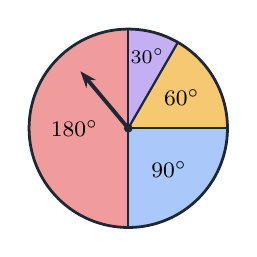
\begin{tikzpicture}[scale=1.05]
\fill[AnsRed!45] (0,0)--(90:1.2) arc (90:270:1.2)--cycle;
\fill[tmBlue!45] (0,0)--(270:1.2) arc (270:360:1.2)--cycle;
\fill[StarGold!70] (0,0)--(0:1.2) arc (0:60:1.2)--cycle;
\fill[tmPurple!45] (0,0)--(60:1.2) arc (60:90:1.2)--cycle;
\draw[Ink,line width=1pt] (0,0) circle (1.2);
\foreach \a in {90,270,0,60}{\draw[Ink,line width=0.8pt] (0,0)--(\a:1.2);}
\node[font=\footnotesize] at (180:0.65){$180^\circ$};
\node[font=\footnotesize] at (315:0.7){$90^\circ$};
\node[font=\footnotesize] at (30:0.75){$60^\circ$};
\node[font=\scriptsize] at (75:0.9){$30^\circ$};
\draw[-{Stealth[length=6pt]},line width=1.4pt,Ink] (0,0)--(130:0.9);\fill[Ink] (0,0) circle (1.5pt);
\end{tikzpicture}
\end{minipage}
\end{probbox}
\probsol{
\textbf{Understanding the problem.} The sectors have \emph{different} sizes, so the four sectors are \emph{not} equally likely. We cannot use ``$1$ sector out of $4$''. Instead, the chance of the arrow stopping in a sector is proportional to the size of the sector, that is, to its central angle.
\begin{recallbox}For a spinner with unequal sectors: $P(\text{sector})=\dfrac{\text{central angle of the sector}}{360^\circ}$. The whole circle has $360^\circ$.\end{recallbox}
\step{1}{Check the data}
$180^\circ+90^\circ+60^\circ+30^\circ=360^\circ$ -- exactly one full circle \checkmark.
\step{2}{Part a}
$P(\text{blue})=\dfrac{90}{360}=\dfrac14$.

\emph{Another way to think:} we can divide the spinner into $12$ equal small sectors of $30^\circ$ each. Then red takes $6$ small sectors, blue $3$, yellow $2$ and purple $1$; these $12$ small sectors are equally likely. $P(\text{blue})=\dfrac{3}{12}=\dfrac14$ \checkmark.
\step{3}{Part b}
The yellow and purple sectors do not overlap, so their total angle is $60^\circ+30^\circ=90^\circ$.
$P(\text{yellow or purple})=\dfrac{90}{360}=\dfrac14$ (or $\dfrac{2+1}{12}=\dfrac{3}{12}=\dfrac14$).
\step{4}{Part c}
Hùng is \textbf{wrong}. The formula ``favourable divided by all'' only works when the outcomes are \emph{equally likely}. Here the four colours are not equally likely: the red sector is half of the spinner, so $P(\text{red})=\dfrac{180}{360}=\dfrac12$, while $P(\text{purple})=\dfrac{30}{360}=\dfrac{1}{12}$ -- very different.
\verify{$P(\text{red})+P(\text{blue})+P(\text{yellow})+P(\text{purple})=\dfrac{6}{12}+\dfrac{3}{12}+\dfrac{2}{12}+\dfrac{1}{12}=1$ \checkmark.}
\begin{parentbox}Cut a paper plate into $12$ equal ``slices of cake'' and colour them as in the problem. Counting the slices of each colour, your child will see at once why a big sector has a big probability.\end{parentbox}
\ans{a) $\dfrac14$;\quad b) $\dfrac14$;\quad c) Wrong, because the sectors are not equal (e.g.\ $P(\text{red})=\dfrac12$, $P(\text{purple})=\dfrac1{12}$).}
}

% ---------------------------------------------------------------- Problem 33
\begin{probbox}{33}{\relax}
The school canteen has this lunch menu: one main dish out of $3$ (chicken rice, phở, bún chả); one drink out of $2$ (iced tea, orange juice); one dessert out of $2$ (chè, yoghurt). Each lunch consists of one main dish, one drink and one dessert.
\begin{enumerate}[label=\alph*),leftmargin=1.5em,itemsep=0pt,topsep=2pt]
\item How many different lunches are there?
\item Lan is given a lunch at random. Find the probability that it includes phở.
\item Find the probability that Lan's lunch includes both phở and orange juice.
\end{enumerate}
\end{probbox}
\probsol{
\textbf{Understanding the problem.} Each lunch is made by three successive choices: main dish, drink, dessert. ``Given at random'' means all the different lunches are equally likely.
\step{1}{Part a -- multiplication rule}
\begin{recallbox}Multiplication rule: if a task has stages with $m$, $n$ and $p$ ways, there are $m\times n\times p$ ways altogether.\end{recallbox}
Number of lunches: $3\times2\times2=12$.
\begin{center}\begin{tikzpicture}[grow'=right,level distance=2.6cm,font=\sffamily\footnotesize,
  every node/.style={draw=tmBlue,fill=tmBlue!8,rounded corners=2pt,inner sep=2pt},
  level 1/.style={sibling distance=2.4cm},level 2/.style={sibling distance=1.2cm},level 3/.style={sibling distance=0.6cm},
  edge from parent/.style={draw=Ink!60}]
\node[fill=Ink!10,draw=Ink]{Lunch}
  child{node{chicken rice} child{node{iced tea} child{node{chè}} child{node{yoghurt}}} child{node{orange juice} child{node{chè}} child{node{yoghurt}}}}
  child{node[fill=tmOrange!25,draw=tmOrange]{phở} child{node{iced tea} child{node{chè}} child{node{yoghurt}}} child{node[fill=tmOrange!25,draw=tmOrange]{orange juice} child{node[fill=tmOrange!25,draw=tmOrange]{chè}} child{node[fill=tmOrange!25,draw=tmOrange]{yoghurt}}}}
  child{node{bún chả} child{node{iced tea} child{node{chè}} child{node{yoghurt}}} child{node{orange juice} child{node{chè}} child{node{yoghurt}}}};
\end{tikzpicture}\end{center}
The tree has $3$ big branches, each splitting into $2$ branches, each of which splits into $2$ again: $12$ end points, exactly $12$ lunches.
\step{2}{Part b}
Lunches with phở: the main dish is fixed as phở, drink $2$ ways, dessert $2$ ways: $1\times2\times2=4$ lunches (the middle branch of the tree).
$P(\text{phở})=\dfrac{4}{12}=\dfrac13$.
\begin{tipbox}A quick way to think: the main dish is chosen at random from $3$ dishes, and each dish appears in the same number of lunches, so $P(\text{phở})=\dfrac13$. The drink and dessert do not matter.\end{tipbox}
\step{3}{Part c}
Main dish phở, drink orange juice, only the dessert is left to choose: $1\times1\times2=2$ lunches (orange in the tree).
$P(\text{phở and orange juice})=\dfrac{2}{12}=\dfrac16$.
\verify{List them: (phở, orange juice, chè) and (phở, orange juice, yoghurt) -- exactly $2$ lunches \checkmark.}
\ans{a) $12$ lunches;\quad b) $\dfrac13$;\quad c) $\dfrac16$.}
}

% ---------------------------------------------------------------- Problem 34
\begin{probbox}{34}{\relax}
A hall has $20$ rows of seats. The first row has $12$ seats, and each row behind has $2$ seats more than the row just in front of it.
\begin{enumerate}[label=\alph*),leftmargin=1.5em,itemsep=0pt,topsep=2pt]
\item How many seats are in row $20$?
\item Which row has exactly $30$ seats?
\item How many seats does the hall have altogether?
\end{enumerate}
\end{probbox}
\probsol{
\textbf{Understanding the problem.} The numbers of seats in the rows are $12,14,16,\dots$ -- an \emph{evenly spaced sequence} with step $d=2$. We need the $20$th term, the position of the term $30$, and the sum of $20$ terms.
\step{1}{Part a -- find the pattern}
\begin{center}
\begin{tabular}{|c|c|c|c|c|c|}\hline
Row & $1$ & $2$ & $3$ & $4$ & $k$\\ \hline
Seats & $12$ & $12+2$ & $12+2\times2$ & $12+3\times2$ & $12+(k-1)\times2$\\ \hline
\end{tabular}
\end{center}
From row $1$ to row $k$ there are $k-1$ ``jumps'', each adding $2$ seats. Row $20$: $12+19\times2=12+38=50$ seats.
\begin{warnbox}Not $12+20\times2=52$: from row $1$ to row $20$ there are only $19$ increases (the ``off by one'' error).\end{warnbox}
\step{2}{Part b}
We need $12+(k-1)\times2=30$, so $(k-1)\times2=18$, $k-1=9$, $k=10$. Row $10$ has $30$ seats.
\step{3}{Part c -- sum of an evenly spaced sequence}
\begin{recallbox}Sum of an evenly spaced sequence $=\dfrac{(\text{first}+\text{last})\times\text{number of terms}}{2}$ (Gauss's pairing method).\end{recallbox}
Total number of seats: $\dfrac{(12+50)\times20}{2}=\dfrac{62\times20}{2}=620$ seats.
\begin{proofbox}Pair row $1$ with row $20$: $12+50=62$; row $2$ with row $19$: $14+48=62$; \ldots; row $10$ with row $11$: $30+32=62$. There are $10$ pairs of $62$ seats each, so the total is $10\times62=620$.\end{proofbox}
\verify{Another way: if every row had $12$ seats there would be $20\times12=240$ seats; the ``extra'' is $0+2+4+\dots+38=2\times(0+1+\dots+19)=2\times190=380$; total $240+380=620$ \checkmark.}
\ans{a) $50$ seats;\quad b) row $10$;\quad c) $620$ seats.}
}

% ---------------------------------------------------------------- Problem 35
\begin{probbox}{35}{\stars{1}}
A box contains only red and blue marbles. If one marble is drawn at random, the probability that it is red is $\dfrac35$. If $5$ more blue marbles are put into the box, the probability of drawing a red marble drops to $\dfrac12$. How many red marbles and how many blue marbles were in the box at the start?
\end{probbox}
\probsol{
\textbf{Understanding the problem.} We do not know the total number of marbles, only \emph{proportions}. Adding blue marbles does not change the number of red marbles. Let us translate the two probabilities into the language of ``equal parts'' (a bar model).
\step{1}{Translate the first condition}
$P(\text{red})=\dfrac35$: if the marbles are split into $5$ equal parts, red takes $3$ parts and blue takes $5-3=2$ parts.
\step{2}{Translate the second condition}
After adding $5$ blue marbles, $P(\text{red})=\dfrac12$: red makes up exactly half, i.e.\ \emph{the number of red marbles equals the number of blue marbles}.
\step{3}{Draw the model and compare}
\begin{figC}
\rowlab{-0.15}{0}{Red}
\blk{0}{1.5}{0}{0.55}{AnsRed}{1 part}\blk{1.5}{3}{0}{0.55}{AnsRed}{1 part}\blk{3}{4.5}{0}{0.55}{AnsRed}{1 part}
\rowlab{-0.15}{-0.8}{Blue}
\blk{0}{1.5}{-0.8}{0.55}{tmBlue}{1 part}\blk{1.5}{3}{-0.8}{0.55}{tmBlue}{1 part}\blk{3}{4.5}{-0.8}{0.55}{tmTeal}{add 5}
\brcdn{3}{4.5}{-1.25}{$1$ part $=5$ marbles}
\end{figC}
Red: $3$ parts. Blue after adding: $2$ parts $+\ 5$ marbles. These are equal, so the $5$ marbles are exactly $3-2=1$ part.
\step{4}{Compute the numbers at the start}
$1$ part $=5$ marbles. Red: $3\times5=15$ marbles. Blue: $2\times5=10$ marbles.
\begin{tipbox}\emph{Algebra version (for those who like it):} let the number of red marbles be $3k$ and blue $2k$. After adding: $3k=2k+5$, so $k=5$.\end{tipbox}
\verify{At the start: $15$ red, $10$ blue, $P(\text{red})=\dfrac{15}{25}=\dfrac35$ \checkmark. Adding $5$ blue: $15$ red, $15$ blue, $P(\text{red})=\dfrac{15}{30}=\dfrac12$ \checkmark.}
\begin{warnbox}Do not try to ``subtract probabilities'': $\dfrac35-\dfrac12=\dfrac1{10}$ tells us nothing directly about the number of marbles. A probability is a \emph{ratio}; go back to actual quantities.\end{warnbox}
\ans{At the start there were $15$ red and $10$ blue marbles.}
}

% ---------------------------------------------------------------- Problem 36
\begin{probbox}{36}{\stars{1}}
Recall: a palindrome is a number that reads the same forwards and backwards (for example $3443$, $7007$).
\begin{enumerate}[label=\alph*),leftmargin=1.5em,itemsep=0pt,topsep=2pt]
\item How many four-digit palindromes are there?
\item How many of them are even?
\item A four-digit palindrome is chosen at random. Find the probability that it is even.
\item Show that every four-digit palindrome is divisible by $11$.
\end{enumerate}
\end{probbox}
\probsol{
\textbf{Understanding the problem.} A four-digit number $\overline{abcd}$ is a palindrome when reading it backwards, $\overline{dcba}$, gives the same number: $d=a$ and $c=b$. So a four-digit palindrome has the form $\overline{abba}$, and only \emph{two} digits are chosen freely: $a$ and $b$.
\step{1}{Part a}
\begin{recallbox}Multiplication rule; the first digit of a number cannot be $0$.\end{recallbox}
\countboxes{digit a/9/from 1 to 9/tmBlue,digit b/10/from 0 to 9/tmOrange,third/1/equals b/tmGreen,fourth/1/equals a/tmGreen}{90}
$a$: $9$ ways ($1$ to $9$); $b$: $10$ ways; the last two digits are forced to equal $b$ and $a$. There are $9\times10=90$ numbers.
\step{2}{Part b}
A number is even when its ones digit is even. The ones digit is $a$, so $a$ must be even \emph{and} non-zero: $a\in\{2,4,6,8\}$ -- $4$ ways. $b$ still has $10$ ways. There are $4\times10=40$ even palindromes.
\begin{warnbox}The digit $0$ is even, but $a=0$ is not allowed because $a$ is also the first digit. So there are $4$, not $5$, choices for $a$.\end{warnbox}
\step{3}{Part c}
$P(\text{even})=\dfrac{40}{90}=\dfrac49$.
\step{4}{Part d -- proof}
\begin{proofbox}Write $\overline{abba}$ using place values:
$\overline{abba}=1000a+100b+10b+a=1001a+110b$.
Since $1001=11\times91$ and $110=11\times10$,
$\overline{abba}=11\times91\times a+11\times10\times b=11\times(91a+10b)$,
which is divisible by $11$.\end{proofbox}
\verify{Examples: $3443=11\times313$; $7007=11\times637$; $1221=11\times111$ \checkmark. Counting check: the palindromes starting with $1$ are $1001,1111,\dots,1991$ -- exactly $10$ numbers; nine first digits give $90$ numbers \checkmark.}
\ans{a) $90$;\quad b) $40$;\quad c) $\dfrac49$;\quad d) $\overline{abba}=11\times(91a+10b)$.}
}

% ---------------------------------------------------------------- Problem 37
\begin{probbox}{37}{\stars{1}}
Using the four digits $0,1,2,3$, four-digit numbers with all digits different are made (each digit used exactly once).
\begin{enumerate}[label=\alph*),leftmargin=1.5em,itemsep=0pt,topsep=2pt]
\item How many such numbers can be made?
\item How many of them are even?
\item One of the numbers from part a) is chosen at random. Find the probability that it is even.
\end{enumerate}
\end{probbox}
\probsol{
\textbf{Understanding the problem.} Each number is an arrangement of the four digits $0,1,2,3$ in the four places (thousands, hundreds, tens, ones), with the condition that the thousands digit is not $0$.
\step{1}{Part a -- choose the restricted position first}
\begin{recallbox}Multiplication rule. A position with a condition is chosen first.\end{recallbox}
\countboxes{thousands/3/1 2 or 3/tmBlue,hundreds/3/0 allowed/tmOrange,tens/2/remaining/tmGreen,ones/1/remaining/tmPurple}{18}
Thousands: $3$ ways ($1$, $2$ or $3$). Hundreds: $3$ digits left (now $0$ may be used): $3$ ways. Tens: $2$ ways. Ones: $1$ way. There are $3\times3\times2\times1=18$ numbers.
\begin{warnbox}Forgetting the condition ``thousands digit not $0$'' gives $4\times3\times2\times1=24$ -- which includes $6$ ``numbers'' starting with $0$, such as $0123$, that are really three-digit numbers.\end{warnbox}
\step{2}{Part b -- split into cases by the ones digit}
An even number ends in $0$ or $2$. These two cases differ because the digit $0$ affects the thousands place.
\begin{itemize}[leftmargin=1.2em,itemsep=1pt,topsep=1pt]
\item \textbf{Case 1: ones digit $0$.} The three digits $1,2,3$ go freely into the other three places (no more worry about $0$ in front): $3\times2\times1=6$ numbers.
\item \textbf{Case 2: ones digit $2$.} $0,1,3$ remain. Thousands not $0$: $2$ ways ($1$ or $3$); hundreds: $2$ ways; tens: $1$ way. There are $2\times2\times1=4$ numbers.
\end{itemize}
\begin{recallbox}Addition rule: for separate cases, add the numbers of ways in each case.\end{recallbox}
Number of even numbers: $6+4=10$.
\step{3}{Part c}
$P(\text{even})=\dfrac{10}{18}=\dfrac59$.
\verify{List the even numbers. Case 1: $1230,1320,2130,2310,3120,3210$ ($6$ numbers). Case 2: $1032,1302,3012,3102$ ($4$ numbers). Total $10$ \checkmark. Odd numbers (ending in $1$ or $3$): each case is like Case 2, with $4$ numbers, total $8$; and $10+8=18$ \checkmark.}
\ans{a) $18$ numbers;\quad b) $10$ even numbers;\quad c) $\dfrac59$.}
}

% ---------------------------------------------------------------- Problem 38
\begin{probbox}{38}{\stars{1}}
\begin{minipage}[t]{0.62\linewidth}\vspace{0pt}
The figure shows a rectangular grid of $2$ rows and $3$ columns of squares.
\begin{enumerate}[label=\alph*),leftmargin=1.5em,itemsep=0pt,topsep=2pt]
\item How many rectangles (including squares) are there in the figure altogether?
\item How many squares are there?
\item One of these rectangles is chosen at random. Find the probability that it is a square.
\end{enumerate}
\end{minipage}\hfill
\begin{minipage}[t]{0.34\linewidth}\vspace{0pt}
\centering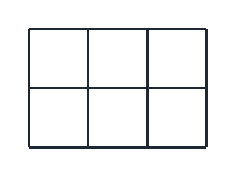
\begin{tikzpicture}[scale=0.75]
\foreach \x in {0,1,2,3}{\draw[Ink,line width=1pt] (\x,0)--(\x,2);}
\foreach \y in {0,1,2}{\draw[Ink,line width=1pt] (0,\y)--(3,\y);}
\end{tikzpicture}
\end{minipage}
\end{probbox}
\probsol{
\textbf{Understanding the problem.} This is a grid with full-length lines, so the ``choose two lines'' trick works. We will also count by size to check.
\step{1}{Part a -- choose two horizontal and two vertical lines}
\begin{recallbox}A rectangle in a grid is determined by $2$ horizontal and $2$ vertical lines. The number of ways to choose $2$ of $n$ lines is $\dfrac{n\times(n-1)}{2}$.\end{recallbox}
The grid has $3$ horizontal and $4$ vertical lines.
\begin{itemize}[leftmargin=1.2em,itemsep=0pt,topsep=1pt]
\item Choose $2$ horizontal lines: $\dfrac{3\times2}{2}=3$ ways.
\item Choose $2$ vertical lines: $\dfrac{4\times3}{2}=6$ ways.
\end{itemize}
By the multiplication rule: $3\times6=18$ rectangles.
\step{2}{Check with a table of sizes}
Write ``height $\times$ width'' (in squares). A shape $w$ squares wide has $4-w$ horizontal positions; $h$ squares high, $3-h$ vertical positions.
\begin{center}
\begin{tabular}{|c|c|c|c|c|c|c|c|}\hline
Size & $1\times1$ & $1\times2$ & $1\times3$ & $2\times1$ & $2\times2$ & $2\times3$ & Total\\ \hline
Number & $2\times3=6$ & $2\times2=4$ & $2\times1=2$ & $1\times3=3$ & $1\times2=2$ & $1\times1=1$ & $18$\\ \hline
\end{tabular}
\end{center}
Both methods give $18$ \checkmark.
\step{3}{Part b}
The squares are the $1\times1$ and $2\times2$ shapes: $6+2=8$ squares.
\begin{warnbox}There is no $3\times3$ square because the grid is only $2$ squares high. And do not forget the two $2\times2$ squares (left and right, overlapping in the middle column).\end{warnbox}
\step{4}{Part c}
$P(\text{square})=\dfrac{8}{18}=\dfrac49$.
\ans{a) $18$;\quad b) $8$;\quad c) $\dfrac49$.}
}

% ---------------------------------------------------------------- Problem 39
\begin{probbox}{39}{\stars{1}}
Four friends An, Bình, Chi and Dũng are seated at random on four chairs in a row.
\begin{enumerate}[label=\alph*),leftmargin=1.5em,itemsep=0pt,topsep=2pt]
\item How many seating arrangements are there?
\item Find the probability that An and Bình sit next to each other.
\item Find the probability that An and Bình sit at the two ends of the row.
\end{enumerate}
\end{probbox}
\probsol{
\textbf{Understanding the problem.} ``Seated at random'' means all arrangements are equally likely. We count all arrangements, then the favourable ones for each event. Number the chairs $1,2,3,4$ from left to right.
\step{1}{Part a}
\begin{recallbox}Seating $n$ people on $n$ chairs: $n\times(n-1)\times\dots\times2\times1$ ways (multiplication rule; each next chair has one person fewer to choose from).\end{recallbox}
Chair $1$: $4$ choices of person; chair $2$: $3$; chair $3$: $2$; chair $4$: $1$. There are $4\times3\times2\times1=24$ arrangements.
\step{2}{Part b -- treat An and Bình as one ``block''}
\begin{figC}
\draw[tmOrange,line width=1.2pt,rounded corners=4pt,fill=tmOrange!12] (0,0) rectangle (2.4,0.7);
\node[font=\bfseries] at (0.6,0.35){An};\node[font=\bfseries] at (1.8,0.35){Bình};
\draw[tmBlue,line width=1pt,rounded corners=3pt,fill=tmBlue!10] (2.7,0) rectangle (3.9,0.7);\node[font=\bfseries] at (3.3,0.35){Chi};
\draw[tmGreen,line width=1pt,rounded corners=3pt,fill=tmGreen!10] (4.2,0) rectangle (5.4,0.7);\node[font=\bfseries] at (4.8,0.35){Dũng};
\node[font=\footnotesize,text=tmOrange!80!black] at (1.2,-0.3){one block, taking $2$ neighbouring chairs};
\end{figC}
\begin{itemize}[leftmargin=1.2em,itemsep=1pt,topsep=1pt]
\item Position of the block (An, Bình): chairs $1$--$2$, $2$--$3$ or $3$--$4$: $3$ ways.
\item Inside the block, An on the left or Bình on the left: $2$ ways.
\item Chi and Dũng on the $2$ remaining chairs: $2\times1=2$ ways.
\end{itemize}
Favourable arrangements: $3\times2\times2=12$. So $P(\text{next to each other})=\dfrac{12}{24}=\dfrac12$.
\begin{warnbox}Do not forget to multiply by $2$ for swapping An and Bình inside the block: ``An--Bình'' and ``Bình--An'' are two different arrangements.\end{warnbox}
\step{3}{Part c}
An and Bình on chairs $1$ and $4$: An on chair $1$ and Bình on chair $4$, or the other way round -- $2$ ways. Chi and Dũng on chairs $2$, $3$: $2$ ways. Favourable arrangements: $2\times2=4$.
$P(\text{both ends})=\dfrac{4}{24}=\dfrac16$.
\verify{Part b, counted another way: if An sits at an end (chair $1$ or $4$, $2$ possibilities) there is only $1$ chair next to An; if An sits in the middle (chair $2$ or $3$) there are $2$ chairs next to An. Number of (An, Bình) neighbouring chair pairs: $2\times1+2\times2=6$; times $2$ ways to seat Chi and Dũng: $12$ \checkmark.}
\begin{parentbox}With $4$ people, let your child use $4$ name cards and actually lay out all $24$ arrangements in order (starting with An, then starting with Bình\ldots). Listing once helps the child trust the multiplication rule.\end{parentbox}
\ans{a) $24$ arrangements;\quad b) $\dfrac12$;\quad c) $\dfrac16$.}
}

% ---------------------------------------------------------------- Problem 40
\begin{probbox}{40}{\stars{2}}
A box contains $4$ red marbles and $6$ blue marbles of the same size. Hoa draws one marble at random, does \emph{not put it back}, and then draws a second marble at random.
\begin{enumerate}[label=\alph*),leftmargin=1.5em,itemsep=0pt,topsep=2pt]
\item Find the probability that both marbles are red.
\item Find the probability that the two marbles have the same colour.
\item Find the probability that the two marbles have different colours.
\end{enumerate}
\end{probbox}
\probsol{
\textbf{Understanding the problem.} Hoa draws two marbles \emph{one after the other} without replacement. Imagine the marbles numbered $1$ to $10$ (marbles $1$--$4$ red, marbles $5$--$10$ blue). Each \emph{ordered pair} (first marble, second marble) is one outcome, and these outcomes are equally likely.
\step{1}{Count all outcomes}
\begin{recallbox}Multiplication rule: the first draw has $10$ ways; for each of them, the second draw has $9$ marbles left, so $9$ ways.\end{recallbox}
Number of outcomes: $10\times9=90$ ordered pairs.
\step{2}{Part a -- both red}
First draw red: $4$ ways. Then $3$ red marbles are left, second draw red: $3$ ways. Favourable outcomes: $4\times3=12$.
$P(\text{red, red})=\dfrac{12}{90}=\dfrac{2}{15}$.
\step{3}{Tree diagram with the numbers of ways}
\begin{center}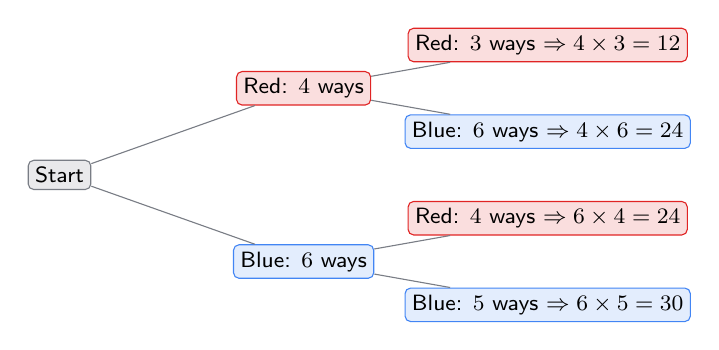
\begin{tikzpicture}[grow'=right,level distance=3.1cm,font=\sffamily\footnotesize,
  every node/.style={draw=Ink!60,rounded corners=2pt,inner sep=2.5pt,fill=white},
  level 1/.style={sibling distance=2.2cm},level 2/.style={sibling distance=1.1cm},
  edge from parent/.style={draw=Ink!60}]
\node[fill=Ink!10]{Start}
  child{node[fill=AnsRed!15,draw=AnsRed]{Red: $4$ ways}
     child{node[fill=AnsRed!15,draw=AnsRed]{Red: $3$ ways $\Rightarrow 4\times3=12$}}
     child{node[fill=tmBlue!15,draw=tmBlue]{Blue: $6$ ways $\Rightarrow 4\times6=24$}}}
  child{node[fill=tmBlue!15,draw=tmBlue]{Blue: $6$ ways}
     child{node[fill=AnsRed!15,draw=AnsRed]{Red: $4$ ways $\Rightarrow 6\times4=24$}}
     child{node[fill=tmBlue!15,draw=tmBlue]{Blue: $5$ ways $\Rightarrow 6\times5=30$}}};
\end{tikzpicture}\end{center}
Check: $12+24+24+30=90$ \checkmark{} -- the four branches cover every outcome.
\step{4}{Part b -- same colour}
Same colour has two separate cases: (red, red) with $12$ outcomes and (blue, blue) with $30$ outcomes.
\begin{recallbox}Addition rule for cases that do not overlap.\end{recallbox}
Favourable outcomes: $12+30=42$. $P(\text{same colour})=\dfrac{42}{90}=\dfrac{7}{15}$.
\step{5}{Part c -- complement}
``Different colours'' is the complement of ``same colour'': $P(\text{different colours})=1-\dfrac{7}{15}=\dfrac{8}{15}$.
\verify{Direct count: (red, blue) $24$ and (blue, red) $24$, total $48$; $\dfrac{48}{90}=\dfrac{8}{15}$ \checkmark.}
\begin{warnbox}The most common mistake: acting as if all $10$ marbles are still there for the second draw, computing $\dfrac{4}{10}\times\dfrac{4}{10}$ or counting $4\times4$ red pairs. Because the marble is \emph{not put back}, the second draw has only $9$ marbles and only $3$ red ones.\end{warnbox}
\begin{tipbox}You can also count without order: the number of ways to choose $2$ of $10$ marbles is $\dfrac{10\times9}{2}=45$, the number of ways to choose $2$ of the $4$ red marbles is $\dfrac{4\times3}{2}=6$, so $P(\text{red, red})=\dfrac{6}{45}=\dfrac{2}{15}$ -- the same result. What matters is that the numerator and denominator are counted \emph{the same way} (both ordered or both unordered).\end{tipbox}
\ans{a) $\dfrac{2}{15}$;\quad b) $\dfrac{7}{15}$;\quad c) $\dfrac{8}{15}$.}
}

% ---------------- part d ----------------
% ================= Topic 3 (EN) -- part d: problems 41--50 (challenge) =================
\begin{probbox}{41}{\stars{1}}
On a square dot grid, Lan stands at dot $A$. She tosses a fair coin $6$ times; each time it shows heads she moves \emph{up} one dot, and
each time it shows tails she moves \emph{right} one dot (as in problem 16). The dots $M$, $N$, $B$ are marked in the figure.
\begin{figC}\begin{scope}[scale=0.85]
  \foreach \x in {0,...,3}{\foreach \y in {0,...,3}{\fill[Navy] (\x,\y) circle (2.4pt);}}
  \fill[tmOrange] (0,0) circle (3.4pt);\node[below left] at (0,0) {$A$};
  \fill[tmGreen!80!black] (1,1) circle (3.4pt);\node[above left] at (1,1) {$M$};
  \fill[AnsRed] (2,1) circle (3.4pt);\node[below right] at (2,1) {$N$};
  \fill[tmPurple] (3,3) circle (3.4pt);\node[above right] at (3,3) {$B$};
\end{scope}\end{figC}
\begin{enumerate}[label=\alph*),leftmargin=1.6em,itemsep=1pt,topsep=2pt]
\item Find the probability that after $6$ tosses Lan stops at dot $B$.
\item Find the probability that Lan passes through dot $M$ \emph{and} stops at $B$.
\item Find the probability that Lan stops at $B$ \emph{without} passing through dot $N$.
\end{enumerate}
\end{probbox}
\probsol{
\textbf{Understanding the problem.} Each sequence of $6$ tosses is a sequence of $6$ symbols $\uparrow$ (up) or $\rightarrow$ (right).
There are $2^6=2\times2\times2\times2\times2\times2=64$ sequences, all equally likely. Each sequence is a \emph{path} on the grid.
We label positions by the pair (number of moves right, number of moves up): $A=(0,0)$, $M=(1,1)$, $N=(2,1)$, $B=(3,3)$.

\step{1}{Count the paths from $A$ to every dot (part a)}
\begin{recallbox}A dot can only be reached from the dot just to its left or the dot just below it. Therefore:
number of paths to a dot $=$ number of paths to the dot on its left $+$ number of paths to the dot below (addition principle).\end{recallbox}
Write the number of paths at each dot, starting from $A$ (write $1$); the bottom row and the left column are all $1$:
\begin{figC}\begin{scope}[scale=0.85]
  \foreach \x/\y/\n in {0/0/1,1/0/1,2/0/1,3/0/1,0/1/1,1/1/2,2/1/3,3/1/4,0/2/1,1/2/3,2/2/6,3/2/10,0/3/1,1/3/4,2/3/10,3/3/20}{
    \fill[tmBlue!12] (\x,\y) circle (9pt);\node[font=\small\bfseries,text=Navy] at (\x,\y) {\n};}
  \draw[tmPurple,thick] (3,3) circle (10pt);\node[right=9pt,text=tmPurple] at (3,3) {$B$};
\end{scope}\end{figC}
There are $20$ paths from $A$ to $B$. (Another way: reaching $B$ needs exactly $3$ up-moves among the $6$ moves; the number of ways to
choose $3$ turns out of $6$ is $\dfrac{6\times5\times4}{3\times2\times1}=20$.)
\[P(a)=\frac{20}{64}=\frac{5}{16}.\]

\step{2}{Part b: through $M$ and then to $B$ -- multiplication principle}
A path through $M$ has two stages: stage $A\to M$ ($1$ up, $1$ right) and stage $M\to B$ ($2$ up, $2$ right).
Stage $A\to M$ can be done in $2$ ways ($\uparrow\rightarrow$ or $\rightarrow\uparrow$); stage $M\to B$ in $6$ ways (as in problem 16:
choose $2$ up-turns out of $4$). Each way of doing the first stage combined with each way of doing the second gives a different path:
$2\times6=12$ paths.
\[P(b)=\frac{12}{64}=\frac{3}{16}.\]

\step{3}{Part c: avoiding $N$ -- use the complement}
Paths from $A$ through $N$ to $B$: stage $A\to N$ ($2$ right, $1$ up) has $3$ ways; stage $N\to B$ ($1$ right, $2$ up) has $3$ ways;
in total $3\times3=9$ paths. So the number of paths from $A$ to $B$ \emph{not} through $N$ is $20-9=11$.
\[P(c)=\frac{11}{64}.\]
\begin{proofbox}\emph{Check by ``blocking'' dot $N$.} Recompute the path numbers but put $0$ at $N$ (as if it cannot be used).
Row $1$: $1,\ 2,\ \mathbf{0},\ 0+1=1$. Row $2$: $1,\ 3,\ 3+0=3,\ 3+1=4$. Row $3$: $1,\ 4,\ 4+3=7,\ 7+4=11$.
At $B$ we get $11$, matching the complement.\end{proofbox}
\begin{warnbox}Parts b and c ask for probabilities among \emph{all} $64$ toss sequences, not among the $20$ paths to $B$. Dividing by $20$
answers a different question (a conditional probability, not yet studied).\end{warnbox}
\verify{In part a the possible final dots are $(6,0),(5,1),\dots,(0,6)$ with $1,6,15,20,15,6,1$ paths; the total is $64$. Dot $B=(3,3)$
corresponds to $20$.}
\ans{a) $\dfrac5{16}$;\quad b) $\dfrac3{16}$;\quad c) $\dfrac{11}{64}$}
}

\begin{probbox}{42}{\stars{2}}
We build grids of squares from toothpicks as in problem 17. An ``$m\times n$'' grid has $m$ rows, each with $n$ squares.
\begin{enumerate}[label=\alph*),leftmargin=1.6em,itemsep=1pt,topsep=2pt]
\item Find a formula for the number of toothpicks needed for an $m\times n$ grid.
\item A square $k\times k$ grid uses exactly $760$ toothpicks. Find $k$.
\item Nam has exactly $2026$ toothpicks and wants to build an $m\times n$ grid (with $1\le m\le n$) that uses \emph{all} of them.
Find all the grids Nam can build.
\end{enumerate}
\end{probbox}
\probsol{
\textbf{Understanding the problem.} As in problem 17, we count horizontal and vertical toothpicks separately. Part c leads to an equation in
two natural-number unknowns; the trick ``multiply by $2$ and add $1$'' turns it into a problem about divisors.

\step{1}{Part a: the formula}
An $m\times n$ grid has $m+1$ horizontal lines of $n$ toothpicks each: $(m+1)\times n$ horizontal toothpicks. It has $n+1$ vertical lines of
$m$ toothpicks each: $(n+1)\times m$ vertical toothpicks. Total:
\[T=(m+1)n+(n+1)m=mn+n+mn+m=2mn+m+n.\]
Check with the $1\times10$ grid: $2\times1\times10+1+10=31$, as in problem 17.

\step{2}{Part b: a square $k\times k$ grid}
Put $m=n=k$: $T=2k^2+2k=2k(k+1)$. We need $2k(k+1)=760$, that is $k(k+1)=380$.
$k(k+1)$ is the product of two consecutive natural numbers. Since $19\times20=380$, $k=19$. (As $k$ grows, $k(k+1)$ grows, so there is only
one value: $18\times19=342<380<420=20\times21$.)

\step{3}{Part c: set up the equation}
We need natural numbers $1\le m\le n$ with $2mn+m+n=2026$.
\begin{tipbox}Multiply both sides by $2$ and add $1$: $4mn+2m+2n+1=4053$. The left side factorises:
$(2m+1)(2n+1)=4mn+2m+2n+1$ (expand to check). So
\[(2m+1)(2n+1)=4053.\]\end{tipbox}

\step{4}{Prime factorisation of $4053$}
The digit sum of $4053$ is $4+0+5+3=12$, divisible by $3$: $4053=3\times1351$. Next, $1351=7\times193$.
The number $193$ is prime: it is not divisible by $2,3,5,7,11,13$, and $13\times13=169<193<196=14\times14$, so no more trials are needed.
\begin{recallbox}To check whether $N$ is prime, it is enough to try dividing by the primes $p$ with $p\times p\le N$.\end{recallbox}
So $4053=3\times7\times193$. The divisors of $4053$ are: $1,\ 3,\ 7,\ 21,\ 193,\ 579,\ 1351,\ 4053$.

\step{5}{Find the pairs $(m,n)$}
Since $m\ge1$, $2m+1\ge3$; since $m\le n$, $2m+1\le2n+1$. The ways of writing $4053$ as a product of two such divisors:
\begin{center}\begin{tabular}{|c|c|c|c|c|}\hline
$2m+1$ & $2n+1$ & $m$ & $n$ & Check $2mn+m+n$\\\hline
$3$ & $1351$ & $1$ & $675$ & $1350+1+675=2026$\\\hline
$7$ & $579$ & $3$ & $289$ & $1734+3+289=2026$\\\hline
$21$ & $193$ & $10$ & $96$ & $1920+10+96=2026$\\\hline
\end{tabular}\end{center}
(The pair $1\times4053$ is rejected because it gives $m=0$.)
\begin{warnbox}Trying $m=1,2,3,\dots$ one by one also works but is very long and it is easy to miss a solution. The ``multiply by $2$, add $1$''
trick turns the problem into ``find the divisors'' and guarantees that \emph{no} solution is missed.\end{warnbox}
\verify{For any other value of $m$, $2m+1$ is not a divisor of $4053$, so $n$ is not a natural number. For example $m=2$: $5(2n+1)=4053$ is
impossible because $4053$ is not divisible by $5$.}
\ans{a) $2mn+m+n$;\quad b) $k=19$;\quad c) three grids: $1\times675$, $3\times289$, $10\times96$}
}

\begin{probbox}{43}{\stars{1}}
Three fair dice coloured red, blue and yellow are rolled together (each is numbered $1$ to $6$). Find the probability of each event:
\begin{enumerate}[label=\alph*),leftmargin=1.6em,itemsep=1pt,topsep=2pt]
\item the three numbers are all different;
\item the number on the red die is less than the number on the blue die, and the number on the blue die is less than the number on the
yellow die;
\item at least one die shows a $6$;
\item the largest of the three numbers is exactly $4$.
\end{enumerate}
\end{probbox}
\probsol{
\textbf{Understanding the problem.} Each outcome is a triple (red, blue, yellow). By the multiplication principle there are
$6\times6\times6=216$ equally likely outcomes.

\step{1}{Part a: three different numbers}
Red die: $6$ ways; blue die different from red: $5$ ways; yellow die different from both: $4$ ways. That gives $6\times5\times4=120$ outcomes.
\[P(a)=\frac{120}{216}=\frac{5}{9}.\]

\step{2}{Part b: red $<$ blue $<$ yellow -- use symmetry}
Take a set of three different numbers, for example $\{2,3,5\}$. There are $3\times2\times1=6$ ways to assign these three numbers to the three
dice ($235$, $253$, $325$, $352$, $523$, $532$), and \emph{exactly one} of them is increasing ($2<3<5$).
So the $120$ outcomes of part a split into groups of $6$, each with $1$ favourable outcome: there are $120\div6=20$ favourable outcomes.
\[P(b)=\frac{20}{216}=\frac{5}{54}.\]
\begin{recallbox}The number of ways to arrange $3$ different objects in $3$ places is $3\times2\times1=6$.\end{recallbox}

\step{3}{Part c: at least one $6$ -- complement}
The opposite event is ``no die shows $6$'': each die has only $5$ outcomes ($1$ to $5$), in total $5\times5\times5=125$.
So the number of outcomes with at least one $6$ is $216-125=91$.
\[P(c)=\frac{91}{216}.\]
\begin{warnbox}Do not argue ``each die shows $6$ with probability $\frac16$, so for three dice it is $\frac36=\frac12$''. That addition counts
twice the outcomes with two or three sixes (for example $(6,6,1)$ is counted twice).\end{warnbox}

\step{4}{Part d: the largest number is exactly $4$}
``Largest number $\le4$'' means all three numbers are in $\{1,2,3,4\}$: $4\times4\times4=64$ outcomes.
``Largest number $\le3$'': $3\times3\times3=27$ outcomes. The largest number is exactly $4$ when it is $\le4$ but not $\le3$:
$64-27=37$ outcomes.
\[P(d)=\frac{37}{216}.\]
\begin{proofbox}Every outcome whose largest number is $\le3$ also belongs to the group whose largest number is $\le4$. Removing the smaller
group leaves exactly the outcomes whose largest number is at most $4$ but more than $3$, that is equal to $4$.\end{proofbox}
\verify{The idea of part d also gives part c: largest number equal to $6$ in $6^3-5^3=216-125=91$ outcomes, a match. The numbers of
outcomes by largest number $1,2,\dots,6$: $1+7+19+37+61+91=216$.}
\ans{a) $\dfrac59$;\quad b) $\dfrac5{54}$;\quad c) $\dfrac{91}{216}$;\quad d) $\dfrac{37}{216}$}
}

\begin{probbox}{44}{\stars{2}}
Special six-sided dice are made with one of the numbers $1,2,3,4,5,6$ written on each face (repeats allowed), so that, as in
problem 19, the probability of rolling a multiple of $3$ is $\frac12$ and the probability of rolling an even number is $\frac13$.
Two dice are considered the same if they carry the same six numbers (regardless of the order of the faces).
\begin{enumerate}[label=\alph*),leftmargin=1.6em,itemsep=1pt,topsep=2pt]
\item What is the largest possible sum of the six numbers on such a die? What is the smallest?
\item How many different such dice are there?
\end{enumerate}
\end{probbox}
\probsol{
\textbf{Understanding the problem.} As in problem 19, the conditions mean: \textbf{exactly $3$ faces are multiples of $3$} and
\textbf{exactly $2$ faces are even}. The key point is that $6$ belongs to both groups, so we sort the numbers $1$--$6$ into four types:
\begin{center}\begin{tabular}{|c|c|c|}\hline
Type & Numbers & Property\\\hline
I & $6$ & even and a multiple of $3$\\\hline
II & $3$ & odd, multiple of $3$\\\hline
III & $2,\ 4$ & even, not a multiple of $3$\\\hline
IV & $1,\ 5$ & odd, not a multiple of $3$\\\hline
\end{tabular}\end{center}

\step{1}{Express the number of faces of each type in terms of the number of $6$s}
Let $a$ be the number of faces showing $6$. Then:
\begin{itemize}[leftmargin=1.2em,itemsep=1pt,topsep=2pt]
\item the number of multiples of $3$ is (type I) $+$ (type II) $=3$, so type II has $3-a$ faces;
\item the number of even faces is (type I) $+$ (type III) $=2$, so type III has $2-a$ faces;
\item type IV has $6-a-(3-a)-(2-a)=1+a$ faces.
\end{itemize}
A number of faces cannot be negative, so $2-a\ge0$, that is $a\in\{0,1,2\}$.
\begin{center}\begin{tabular}{|c|c|c|c|c|}\hline
$a$ & type I (the $6$s) & type II (the $3$s) & type III ($2$ or $4$) & type IV ($1$ or $5$)\\\hline
$0$ & $0$ & $3$ & $2$ & $1$\\\hline
$1$ & $1$ & $2$ & $1$ & $2$\\\hline
$2$ & $2$ & $1$ & $0$ & $3$\\\hline
\end{tabular}\end{center}

\step{2}{Part a: largest and smallest sums}
For the largest sum, choose all $4$s in type III and all $5$s in type IV. The sum is
\[6a+3(3-a)+4(2-a)+5(1+a)=22+4a,\]
largest when $a=2$: sum $30$ (the die $3,5,5,5,6,6$).
For the smallest sum, choose all $2$s in type III and all $1$s in type IV. The sum is
\[6a+3(3-a)+2(2-a)+1\cdot(1+a)=14+2a,\]
smallest when $a=0$: sum $14$ (the die $1,2,2,3,3,3$).
\begin{recallbox}Collecting terms: $6a-3a-4a+5a=4a$ and $9+8+5=22$; similarly $6a-3a-2a+a=2a$ and $9+4+1=14$.\end{recallbox}

\step{3}{Part b: count the dice}
Once $a$ is known, we only have to decide how many of the type III faces are $4$ (the rest are $2$), and how many of the type IV faces are
$5$ (the rest are $1$).
\begin{itemize}[leftmargin=1.2em,itemsep=1pt,topsep=2pt]
\item $a=0$: type III has $2$ faces, the number of $4$s can be $0,1,2$: $3$ ways; type IV has $1$ face: $2$ ways. That gives $3\times2=6$ dice.
\item $a=1$: type III has $1$ face: $2$ ways; type IV has $2$ faces: $3$ ways. That gives $2\times3=6$ dice.
\item $a=2$: type III has $0$ faces: $1$ way; type IV has $3$ faces (the number of $5$s is $0,1,2,3$): $4$ ways. That gives $1\times4=4$ dice.
\end{itemize}
Total: $6+6+4=16$ dice.
\begin{warnbox}Since the order of the faces does not matter, two type III faces ``$2,4$'' or ``$4,2$'' are \emph{one} case. Counting the
\emph{number} of $4$s ($0$, $1$ or $2$) instead of arranging them avoids double counting.\end{warnbox}
\verify{Two dice from the list: with $a=1$, one $4$ and two $1$s: the die $1,1,3,3,4,6$ has $3$ multiples of $3$ ($3,3,6$) and $2$ even
faces ($4,6$). Correct. The die $1,2,2,3,3,3$ (sum $14$) also has $3$ multiples of $3$ and $2$ even faces.}
\ans{a) Largest $30$, smallest $14$;\quad b) $16$ dice}
}

\begin{probbox}{45}{\stars{1}}
Three lights flash: the first flashes every $4$ seconds, the second every $6$ seconds, the third every $10$ seconds. At the start
($0$ seconds) all three flash together. Consider the next $10$ minutes (from second $1$ to the end of second $600$).
\begin{enumerate}[label=\alph*),leftmargin=1.6em,itemsep=1pt,topsep=2pt]
\item How many times do all three lights flash together?
\item At how many moments do \emph{exactly two} lights flash together?
\item At how many moments does at least one light flash?
\end{enumerate}
\end{probbox}
\probsol{
\textbf{Understanding the problem.} The first light flashes at the seconds that are multiples of $4$; the second at multiples of $6$; the
third at multiples of $10$ (as in problem 20, but here every multiple counts, not only odd multiples). We count multiples from $1$ to $600$.

\step{1}{Count how many times each light flashes}
\begin{recallbox}The number of multiples of $d$ among $1$ to $N$ is the whole-number part of $N\div d$ (the quotient in division with
remainder).\end{recallbox}
Light 1: $600\div4=150$ times. Light 2: $600\div6=100$ times. Light 3: $600\div10=60$ times.

\step{2}{Two and three lights together -- use the LCM}
Two lights flash together when the number of seconds is a common multiple of the two periods, that is a multiple of their LCM.
\begin{itemize}[leftmargin=1.2em,itemsep=1pt,topsep=2pt]
\item $\text{lcm}(4,6)=12$: $600\div12=50$ times lights 1 and 2 flash together.
\item $\text{lcm}(4,10)=20$: $600\div20=30$ times.
\item $\text{lcm}(6,10)=30$: $600\div30=20$ times.
\item $\text{lcm}(4,6,10)=60$: $600\div60=10$ times all three flash together. This answers part a.
\end{itemize}
\begin{warnbox}$\text{lcm}(4,6)$ is $12$, not $4\times6=24$ (because $4$ and $6$ have the common divisor $2$). Similarly
$\text{lcm}(4,6,10)=60$, not $240$.\end{warnbox}

\step{3}{Part b: exactly two lights}
Of the $50$ times lights 1 and 2 flash together, light 3 also flashes $10$ times (all three), so only lights 1 and 2 flash $50-10=40$ times.
Similarly: only lights 1 and 3: $30-10=20$; only lights 2 and 3: $20-10=10$. Total number of moments with exactly two lights:
$40+20+10=70$.

\step{4}{Part c: draw a Venn diagram and fill it in from the inside out}
Only light 1: $150-40-20-10=80$; only light 2: $100-40-10-10=40$; only light 3: $60-20-10-10=20$.
\begin{figC}
  \fill[tmBlue,opacity=0.12] (0,0) circle (1.3);\fill[tmOrange,opacity=0.12] (1.6,0) circle (1.3);
  \fill[tmGreen,opacity=0.12] (0.8,-1.3) circle (1.3);
  \draw[tmBlue,thick] (0,0) circle (1.3);\draw[tmOrange,thick] (1.6,0) circle (1.3);\draw[tmGreen!80!black,thick] (0.8,-1.3) circle (1.3);
  \node[text=tmBlue] at (-0.9,1.25) {light 1};\node[text=tmOrange!80!black] at (2.6,1.25) {light 2};
  \node[text=tmGreen!70!black] at (0.8,-2.85) {light 3};
  \node at (-0.45,0.25) {$80$};\node at (2.05,0.25) {$40$};\node at (0.8,-1.95) {$20$};
  \node at (0.8,0.5) {$40$};\node at (0.05,-0.95) {$20$};\node at (1.55,-0.95) {$10$};
  \node[text=AnsRed,font=\bfseries\small] at (0.8,-0.45) {$10$};
\end{figC}
The number of moments when at least one light flashes is the sum of the seven numbers in the diagram:
\[80+40+20+40+20+10+10=220.\]
\begin{recallbox}\emph{Inclusion--exclusion} for three groups: number of elements in at least one group $=$ (sum of the sizes of the three groups)
$-$ (sum of the sizes of the overlaps of each pair of groups) $+$ (size of the overlap of all three groups). The overlap of all three is added
$3$ times and subtracted $3$ times, so it must be added back once.\end{recallbox}
\verify{By inclusion--exclusion: $150+100+60-50-30-20+10=220$. It matches the Venn diagram.}
\ans{a) $10$ times;\quad b) $70$ moments;\quad c) $220$ moments}
}

\begin{probbox}{46}{\stars{2}}
\begin{enumerate}[label=\alph*),leftmargin=1.6em,itemsep=2pt,topsep=2pt]
\item A square pyramid has $5$ faces: a square base and four triangular side faces. What is the smallest number of colours needed to paint
the $5$ faces (one colour per face) so that any two faces sharing an edge have different colours?
\item There are $6$ different colours. We paint the six faces of a cube, one colour per face, using all $6$ colours. Two cubes are considered
the same if one can be rotated to look exactly like the other. How many different cubes are there?
\end{enumerate}
\begin{figC}
  \begin{scope}
    \coordinate (A) at (0,0);\coordinate (B) at (2,0);\coordinate (C) at (2.7,0.6);\coordinate (D) at (0.7,0.6);\coordinate (S) at (1.35,2.1);
    \draw[Ink,thick,dashed] (A)--(D)--(C);\draw[Ink,thick,dashed] (D)--(S);
    \fill[tmBlue!30] (A)--(B)--(S)--cycle;\fill[tmOrange!35] (B)--(C)--(S)--cycle;
    \draw[Ink,thick] (A)--(B)--(C)--(S)--cycle;\draw[Ink,thick] (B)--(S);
    \node[font=\scriptsize] at (1.35,-0.3) {square pyramid};
  \end{scope}
  \begin{scope}[shift={(4.2,0)}]
    \fill[tmGreen!35,draw=Ink,thick] (0,0)--(1.4,0)--(1.4,1.4)--(0,1.4)--cycle;
    \fill[tmPurple!30,draw=Ink,thick] (0,1.4)--(1.4,1.4)--(2.0,1.95)--(0.6,1.95)--cycle;
    \fill[tmTeal!30,draw=Ink,thick] (1.4,0)--(2.0,0.55)--(2.0,1.95)--(1.4,1.4)--cycle;
    \node[font=\scriptsize] at (1,-0.3) {cube with $6$ colours};
  \end{scope}
\end{figC}
\end{probbox}
\probsol{
\textbf{Understanding the problem.} Part a is like problem 21: find a colouring and prove that fewer colours are impossible. Part b is a
counting problem ``up to rotation'': we must be careful because a cube can be placed in many positions.

\step{1}{Part a: at least $3$ colours are needed}
\begin{proofbox}The base shares an edge with all four side faces, so its colour differs from the colour of every side face. Two neighbouring
side faces also share an edge (a slanted edge going up to the apex), so they must differ too. Take the base and two neighbouring side faces:
any two of these three faces share an edge, so at least $3$ colours are needed.\end{proofbox}
\emph{Three colours are enough:} paint the base colour $1$; going around, paint the four side faces alternately colour $2$, colour $3$,
colour $2$, colour $3$. The fourth side face (colour $3$) is next to the first (colour $2$): different. So part a needs at least $3$ colours.
\begin{tipbox}If the base were a pentagon (a pyramid with $5$ side faces), the $5$ side faces would form an odd ring and could not alternate
between two colours, so $4$ colours would be needed. Whether the number of side faces is even or odd decides the answer!\end{tipbox}

\step{2}{Part b: put the cube in a ``standard position''}
Call the colours $1,2,3,4,5,6$. Rotate each cube in two steps:
\begin{itemize}[leftmargin=1.2em,itemsep=1pt,topsep=2pt]
\item rotate it so that the face of colour $1$ is \emph{at the bottom};
\item keeping the bottom fixed, turn it about the vertical axis so that, among the four side faces, the one with the \emph{smallest colour
number} is at the front.
\end{itemize}
Once placed like this, no rotation keeps both the bottom face and the front face in place. Therefore two cubes are the same exactly when,
in standard position, they have the same colour in every position.

\step{3}{Count the standard positions}
\begin{itemize}[leftmargin=1.2em,itemsep=1pt,topsep=2pt]
\item Top face (opposite colour $1$): one of the $5$ remaining colours: $5$ ways.
\item The four remaining colours go on the four side faces; the smallest of them is already placed at the front (no choice).
\item The other three colours go on the three faces left, back, right: $3\times2\times1=6$ ways.
\end{itemize}
By the multiplication principle: $5\times6=30$ different cubes.

\step{4}{Check with a second method}
If rotations were \emph{not} allowed (the six positions top, bottom, front, back, left, right fixed), the number of paintings would be
$6\times5\times4\times3\times2\times1=720$. Each cube can be placed in $6\times4=24$ positions ($6$ choices for the face at the bottom, then
$4$ turns about the vertical axis), and with $6$ different colours these $24$ positions give $24$ different fixed paintings.
So the number of different cubes is $720\div24=30$.
\begin{warnbox}Answering $720$ forgets that cubes which can be rotated into each other are the same. Answering $6\times5=30$ ``by luck''
without explanation is not enough either: you must argue why each cube is counted exactly once.\end{warnbox}
\verify{The two counts (standard position and dividing by $24$) give the same result, $30$.}
\ans{a) $3$ colours;\quad b) $30$ cubes}
}

\begin{probbox}{47}{\stars{2}}
Consider the integers $1,2,3,\dots,20$.
\begin{enumerate}[label=\alph*),leftmargin=1.6em,itemsep=1pt,topsep=2pt]
\item How many pairs $(m,n)$ with $m<n$ are there such that $m+n$ is divisible by $3$?
\item How many pairs $(m,n)$ with $m<n$ are there such that $m+n$ is divisible by $4$?
\item How many triples $(m,n,p)$ with $m<n<p$ are there such that $m+n+p$ is divisible by $3$?
\end{enumerate}
\end{probbox}
\probsol{
\textbf{Understanding the problem.} In problem 22 we sorted the numbers by parity (the remainder on division by $2$). Here we sort them by
\emph{the remainder on division by $3$} (or by $4$). Because $m<n$ (and $m<n<p$), each pair or triple is counted once, regardless of order.
\begin{recallbox}The remainder of a sum on division by $3$ equals the remainder of the sum of the remainders. For example $7+11=18$: $7$ leaves
remainder $1$, $11$ leaves remainder $2$, $1+2=3$ is divisible by $3$, so $18$ is divisible by $3$.\end{recallbox}

\step{1}{Sort the $20$ numbers by remainder on division by $3$}
\begin{center}\begin{tabular}{|c|l|c|}\hline
Remainder & Numbers & How many\\\hline
$0$ & $3,6,9,12,15,18$ & $6$\\\hline
$1$ & $1,4,7,10,13,16,19$ & $7$\\\hline
$2$ & $2,5,8,11,14,17,20$ & $7$\\\hline
\end{tabular}\end{center}

\step{2}{Part a}
The sum of two remainders is divisible by $3$ in only two cases: $0+0$ or $1+2$.
\begin{itemize}[leftmargin=1.2em,itemsep=1pt,topsep=2pt]
\item Both numbers with remainder $0$: choose $2$ of the $6$ numbers: $\dfrac{6\times5}{2}=15$ pairs.
\item One with remainder $1$, one with remainder $2$: $7\times7=49$ pairs (the numbers are in different groups, so automatically different;
the smaller one is $m$).
\end{itemize}
(Two numbers with remainder $1$ give a sum with remainder $2$; two numbers with remainder $2$ give $4$, remainder $1$: not allowed.)
Total: $15+49=64$ pairs.

\step{3}{Part b: sort by remainder on division by $4$}
Each remainder $0,1,2,3$ has exactly $5$ numbers (because $20=4\times5$). The sum of two remainders is divisible by $4$ for: $0+0$, $2+2$
or $1+3$.
\[\frac{5\times4}{2}+\frac{5\times4}{2}+5\times5=10+10+25=45 \text{ pairs.}\]

\step{4}{Part c: the remainder patterns of a triple}
List every pattern of remainders (order not important) of three numbers and its sum:
\begin{center}\begin{tabular}{|c|c|c|c|c|c|c|c|c|c|c|}\hline
Pattern & $000$ & $111$ & $222$ & $012$ & $001$ & $002$ & $011$ & $022$ & $112$ & $122$\\\hline
Sum & $0$ & $3$ & $6$ & $3$ & $1$ & $2$ & $2$ & $4$ & $4$ & $5$\\\hline
Divisible by $3$? & yes & yes & yes & yes & no & no & no & no & no & no\\\hline
\end{tabular}\end{center}
Count the four good patterns:
\begin{itemize}[leftmargin=1.2em,itemsep=1pt,topsep=2pt]
\item Pattern $000$: choose $3$ of $6$ numbers: $\dfrac{6\times5\times4}{3\times2\times1}=20$.
\item Pattern $111$: choose $3$ of $7$ numbers: $\dfrac{7\times6\times5}{3\times2\times1}=35$. Pattern $222$: also $35$.
\item Pattern $012$: one number from each group: $6\times7\times7=294$.
\end{itemize}
Total: $20+35+35+294=384$ triples.
\begin{recallbox}The number of ways to choose $3$ objects (order not important) from $k$ objects is $\dfrac{k\times(k-1)\times(k-2)}{6}$:
there are $k(k-1)(k-2)$ ordered choices, and each triple is counted $3\times2\times1=6$ times.\end{recallbox}
\begin{warnbox}For pattern $012$ we do \emph{not} divide by $6$: the three numbers come from three different groups, so each choice (one number
with remainder $0$, one with remainder $1$, one with remainder $2$) gives exactly one triple, which we then write in increasing order.\end{warnbox}
\verify{The total number of triples is $\dfrac{20\times19\times18}{6}=1140$. There are $384$ triples with sum divisible by $3$, close to
$\dfrac13$ of $1140$ ($380$), which is reasonable since the sums are spread ``fairly evenly'' among the three remainders.}
\ans{a) $64$ pairs;\quad b) $45$ pairs;\quad c) $384$ triples}
}

\begin{probbox}{48}{\stars{1}}
For a two-digit number $n=\nd{ab}$, call $\nd{ba}$ the \emph{reversal} of $n$ (as in problem 23).
\begin{enumerate}[label=\alph*),leftmargin=1.6em,itemsep=1pt,topsep=2pt]
\item Find all two-digit numbers $n$ such that $n$ plus its reversal is a perfect square.
\item Find all two-digit numbers with both digits non-zero such that $n$ minus its reversal is a positive perfect square.
\item Prove that every four-digit number of the form $\nd{abba}$ (a palindrome) is divisible by $11$.
\end{enumerate}
\end{probbox}
\probsol{
\textbf{Understanding the problem.} Write the numbers in terms of their digits: $\nd{ab}=10a+b$ and $\nd{ba}=10b+a$, where $a$ is the tens digit
($1\le a\le9$) and $b$ is the units digit. A perfect square is the square of a natural number: $1,4,9,16,25,\dots$

\step{1}{Part a: compute the sum}
$\nd{ab}+\nd{ba}=(10a+b)+(10b+a)=11a+11b=11(a+b)$.
\begin{proofbox}If $11(a+b)=s\times s$, then $s\times s$ is divisible by the prime $11$, so $s$ is divisible by $11$ (if a product of two numbers
is divisible by a prime $p$, one of the two numbers is divisible by $p$). Then $s\times s$ is divisible by $121$, so $11(a+b)$ is divisible by
$121$, and $a+b$ is divisible by $11$.\end{proofbox}
For a two-digit number (the reversal may start with $0$, e.g.\ $\nd{ba}=b$ when $b=0$) we have $1\le a+b\le18$, so $a+b=11$, and then the
sum is $11\times11=121=11^2$, which is indeed a perfect square. The numbers are those with $a+b=11$, $a$ from $2$ to $9$:
\[29,\ 38,\ 47,\ 56,\ 65,\ 74,\ 83,\ 92 \quad(8 \text{ numbers}).\]

\step{2}{Part b: compute the difference}
$\nd{ab}-\nd{ba}=(10a+b)-(10b+a)=9a-9b=9(a-b)$. The difference is positive, so $a>b\ge1$.
Since $9=3\times3$ is a perfect square, $9(a-b)$ is a perfect square exactly when $a-b$ is a perfect square.
\begin{proofbox}If $a-b=t\times t$, then $9(a-b)=(3t)\times(3t)$. Conversely, if $9(a-b)=s\times s$, then $s\times s$ is divisible by $3$, so
$s$ is divisible by $3$; writing $s=3t$ gives $9(a-b)=9t\times t$, that is $a-b=t\times t$.\end{proofbox}
Since $1\le b<a\le9$, we have $1\le a-b\le8$; the perfect squares in this range are $1$ and $4$.
\begin{itemize}[leftmargin=1.2em,itemsep=1pt,topsep=2pt]
\item $a-b=1$: $21, 32, 43, 54, 65, 76, 87, 98$ ($8$ numbers).
\item $a-b=4$: $51, 62, 73, 84, 95$ ($5$ numbers).
\end{itemize}
There are $13$ numbers in all.

\step{3}{Part c: split by place value}
\[\nd{abba}=1000a+100b+10b+a=1001a+110b=11\times91\times a+11\times10\times b=11\times(91a+10b).\]
So $\nd{abba}$ is always divisible by $11$.
\begin{warnbox}$\nd{ab}$ denotes the number with digits $a$ and $b$, \emph{not} the product $a\times b$. Always rewrite $\nd{ab}$ as $10a+b$
before calculating.\end{warnbox}
\verify{a) $47+74=121=11^2$. b) $73-37=36=6^2$, $98-89=9=3^2$. c) $2332=11\times212$, $7007=11\times637$.}
\ans{a) $29$, $38$, $47$, $56$, $65$, $74$, $83$, $92$;\quad b) $13$ numbers (listed in step 2);\quad c) see the proof.}
}

\begin{probbox}{49}{\stars{2}}
A grid of $3$ rows and $5$ columns of squares ($15$ small squares) is shown; the square in the very centre is shaded.
\begin{figC}\begin{scope}[scale=0.6]
  \fill[tmOrange!45] (2,1) rectangle (3,2);
  \draw[Ink,thick] (0,0) grid (5,3);
\end{scope}\end{figC}
\begin{enumerate}[label=\alph*),leftmargin=1.6em,itemsep=1pt,topsep=2pt]
\item How many rectangles (including squares) with sides on the grid lines are there in the figure?
\item How many of them are squares?
\item One of the rectangles in part a is chosen at random. Find the probability that it contains the shaded square.
\end{enumerate}
\end{probbox}
\probsol{
\textbf{Understanding the problem.} As in problem 24, each rectangle is determined by two horizontal grid lines (top and bottom sides) and
two vertical grid lines (left and right sides). A grid with $3$ rows has $4$ horizontal lines, numbered $0,1,2,3$ from top to bottom; a grid
with $5$ columns has $6$ vertical lines, numbered $0,1,\dots,5$ from left to right.

\step{1}{Part a: count the rectangles}
Choose $2$ of the $4$ horizontal lines: $\dfrac{4\times3}{2}=6$ ways. Choose $2$ of the $6$ vertical lines: $\dfrac{6\times5}{2}=15$ ways.
By the multiplication principle: $6\times15=90$ rectangles.

\step{2}{Part b: count the squares by size}
\begin{recallbox}In a $3\times5$ grid, a square of side $k$ has $(3-k+1)$ positions vertically and $(5-k+1)$ positions horizontally.\end{recallbox}
\begin{itemize}[leftmargin=1.2em,itemsep=1pt,topsep=2pt]
\item side $1$: $3\times5=15$ squares;
\item side $2$: $2\times4=8$ squares;
\item side $3$: $1\times3=3$ squares;
\item side $4$ or more: none (the grid is only $3$ high).
\end{itemize}
Total: $15+8+3=26$ squares.
\begin{warnbox}Do not use ``choose $2$ horizontal and $2$ vertical lines'' to count squares: most of those choices give rectangles that are not
squares. Squares must be counted by side length.\end{warnbox}

\step{3}{Part c: rectangles containing the centre square}
The centre square lies between horizontal lines $1$ and $2$, and between vertical lines $2$ and $3$. A rectangle contains it exactly when:
\begin{itemize}[leftmargin=1.2em,itemsep=1pt,topsep=2pt]
\item its top side is horizontal line $0$ or $1$ (above the square): $2$ ways; its bottom side is horizontal line $2$ or $3$: $2$ ways;
\item its left side is vertical line $0$, $1$ or $2$: $3$ ways; its right side is vertical line $3$, $4$ or $5$: $3$ ways.
\end{itemize}
\begin{figC}\begin{scope}[scale=0.6]
  \fill[tmGreen!25] (1,0) rectangle (4,2);
  \fill[tmOrange!55] (2,1) rectangle (3,2);
  \draw[Ink,thick] (0,0) grid (5,3);
  \draw[tmGreen!70!black,line width=2pt] (1,0) rectangle (4,2);
  \foreach \i in {0,...,5}{\node[font=\scriptsize,text=Slate] at (\i,3.35) {\i};}
  \foreach \j/\l in {3/0,2/1,1/2,0/3}{\node[font=\scriptsize,text=Slate] at (-0.35,\j) {\l};}
\end{scope}\end{figC}
(For example, the green rectangle: top side horizontal line $1$, bottom side horizontal line $3$, left side vertical line $1$, right side
vertical line $4$.)
Number of rectangles containing the centre square: $2\times2\times3\times3=36$.
\[P=\frac{36}{90}=\frac{2}{5}.\]
\begin{proofbox}Why is this condition right? A rectangle contains the centre square exactly when it ``covers'' that square in both directions:
its top side must be above (or on) the top side of the square, its bottom side below (or on) the bottom side of the square; similarly for the
left and right sides. These four choices are independent, so we multiply.\end{proofbox}
\verify{Split by direction: of the $15$ choices of two vertical lines, $3\times3=9$ ``cover'' the middle column; of the $6$ choices of two
horizontal lines, $2\times2=4$ cover the middle row. Probability $=\dfrac{9}{15}\times\dfrac{4}{6}=\dfrac35\times\dfrac23=\dfrac25$. It matches.}
\ans{a) $90$;\quad b) $26$;\quad c) $\dfrac25$}
}

\begin{probbox}{50}{\stars{2}}
A box contains $2026$ red marbles and $2027$ blue marbles. Outside the box there is a very large pile of blue marbles. Phong repeats the
following step: take $2$ marbles from the box at random.
\begin{itemize}[leftmargin=1.2em,itemsep=1pt,topsep=2pt]
\item If the two marbles have the \emph{same colour} (both red or both blue): throw both away, then take $1$ blue marble from the pile
outside and put it into the box.
\item If the two marbles have \emph{different colours}: throw away the blue one and put the red one back into the box.
\end{itemize}
Phong stops when only $1$ marble is left in the box.
\begin{enumerate}[label=\alph*),leftmargin=1.6em,itemsep=1pt,topsep=2pt]
\item How many steps did Phong carry out?
\item Find the probability that the last marble is red.
\item If the box had started with $2025$ red marbles and $2027$ blue marbles, what would the probability in part b be?
\end{enumerate}
\end{probbox}
\probsol{
\textbf{Understanding the problem.} There are thousands of marbles, so we cannot draw a probability tree as in problem 25. Instead we look for
a quantity that \emph{does not change} in any step (called an \emph{invariant}). In problem 25 the invariant was ``there is always a blue
marble''; here we look at \emph{the parity of the number of red marbles}.

\step{1}{Part a: each step reduces the number of marbles by exactly $1$}
\begin{itemize}[leftmargin=1.2em,itemsep=1pt,topsep=2pt]
\item Same colour: $2$ taken out, $1$ put in $\Rightarrow$ the number of marbles in the box decreases by $1$.
\item Different colours: $2$ taken out, $1$ put back $\Rightarrow$ the number decreases by $1$.
\end{itemize}
At the start there are $2026+2027=4053$ marbles, and at the end $1$ marble is left. The number of steps is $4053-1=4052$.

\step{2}{Follow the number of red marbles in each case}
\begin{center}\begin{tabular}{|c|c|c|}\hline
Drawn & Change in red marbles & Change in blue marbles\\\hline
red, red & decreases by $2$ & increases by $1$\\\hline
blue, blue & no change & down $2$, up $1$: decreases by $1$\\\hline
red, blue & no change (the red is put back) & decreases by $1$\\\hline
\end{tabular}\end{center}
\begin{proofbox}The number of red marbles either stays the same or decreases by exactly $2$. Subtracting $2$ does not change parity (an even
number minus $2$ is still even, an odd number minus $2$ is still odd). So \textbf{the parity of the number of red marbles never changes}, no
matter which marbles Phong draws.\end{proofbox}

\step{3}{Part b: $2026$ red marbles at the start (an even number)}
The number of red marbles is always even. When only $1$ marble is left: if it were red, the number of red marbles would be $1$ (odd) --
impossible. So the last marble is certainly blue. The event ``the last marble is red'' is an impossible event:
\[P(\text{last marble red})=0.\]

\step{4}{Part c: $2025$ red marbles at the start (an odd number)}
The number of red marbles is always odd, so it is never $0$. When $1$ marble is left, the number of red marbles is an odd number not exceeding
$1$, that is $1$: the last marble is certainly red. This is a certain event:
\[P(\text{last marble red})=1.\]
\begin{tipbox}The initial number of blue marbles has no effect on the result! Only the parity of the number of red marbles decides the colour
of the last marble.\end{tipbox}
\begin{parentbox}Play with your child using a few marbles (for example $2$ red and $3$ blue, or $3$ red and $2$ blue), or with coins of two
colours. Seeing the same result every time makes children curious about ``why''; then give a hint: ``Try counting the red marbles after each
turn: is the number even or odd?''\end{parentbox}
\begin{warnbox}Seeing the word ``random'' and thinking the answer must be a ``nice'' fraction such as $\frac12$ is a mistake. Some random
processes have a final result that is completely determined.\end{warnbox}
\verify{Try $2$ red, $1$ blue: drawing red--red $\to(0\text{ red},2\text{ blue})\to(0,1)$: blue; drawing red--blue $\to(2,0)\to$ draw
red--red $\to(0,1)$: blue. Every way ends with a blue marble, consistent with an even initial number of red marbles.}
\ans{a) $4052$ steps;\quad b) $0$;\quad c) $1$}
}

\end{document}
